% !TeX spellcheck = en_US
% Review Christian Stary January 2020
% Merge mit Thomas Schaller Pfad Chapter 4

% testcomment

\RequirePackage{snapshot}

\documentclass[11pt, showtrims, final, oldfontcommands]{memoir}
% Resolve conflict between functions in class memoir and package changes
\let\classadded\added 	 % save the class’ definition
\let\added\relax		 % ‘undefine’ \foo
\let\deleted\relax    % neutralize \deleted command
\let\comment\relax    % neutralize \comment command



\usepackage[T1]{fontenc}
\usepackage[textsize=footnotesize]{todonotes}

\usepackage{morewrites}

% prepare package changes for managing the review process
\usepackage[draft, markup=underlined, highlightmarkup=background]{changes}
\definechangesauthor[name= Albert Fleischmann, color=green]{AF}
\definechangesauthor[name= Werner Schmidt, color=blue]{WS}
\definechangesauthor[name= Robert Singer, color=cyan]{RS}
\definechangesauthor[name= Christian Stary, color=purple]{CS}
\definechangesauthor[name= Andre Wolski, color=magenta]{AW}
\definechangesauthor[name= Stephan Borgert, color=orange]{SB}
\definechangesauthor[name= Matthes Elstermann, color=pink]{ME}
\definechangesauthor[name= Thomas Schaller, color=violet]{TS}
\definechangesauthor[name= alle anderen, color=lightgray]{STAR}

\usepackage{soulutf8}
\usepackage{soul}

\usepackage{memsty}
\usepackage{memlays}
\usepackage{titlepages}
\usepackage{dpfloat}
\usepackage{fonttable}[2009/04/01]
\usepackage{sidecap}
\usepackage{wrapfig}
\usepackage[htt]{hyphenat}
\usepackage{lscape}
\usepackage{listings}
\usepackage{enumitem}
\usepackage{longtable}
\usepackage{pdfpages}
\usepackage{caption}

\usepackage{amssymb}
\usepackage{program}
\usepackage{mathtools}
\usepackage{graphicx}
\usepackage{minted}

\usepackage{xargs}                      % Use more than one optional parameter in a new commands
\usepackage{xcolor}  % Coloured text etc.









\newmintinline[asminline]{lexer.py:CoreASMLexer -x}{escapeinside=~~}

\setlistdepth{9}

\setlist[itemize,1]{label=$\bullet$}
\setlist[itemize,2]{label=$\bullet$}
\setlist[itemize,3]{label=$\bullet$}
\setlist[itemize,4]{label=$\bullet$}
\setlist[itemize,5]{label=$\bullet$}
\setlist[itemize,6]{label=$\bullet$}
\setlist[itemize,7]{label=$\bullet$}
\setlist[itemize,8]{label=$\bullet$}
\setlist[itemize,9]{label=$\bullet$}

\renewlist{itemize}{itemize}{9}

% Use the built-in division styling
\headstyles{memman}

% BoD bietet zwei Grossformate an: A4 und etwas kleiner
% Springer empfiehlt 24 x 17
\setstocksize{29.7cm}{21cm}

% size of the page after trimming the typeblock
% Springer Textfeld inkl. Kopfzeile 20.5 x 13.5
\settrimmedsize{29.7cm}{21.0cm}{*}

% lines of text
\settypeblocksize{50\onelineskip}{32pc}{*}

% Stocksize ist deckungsgleich mit Druckbereich
\setlength{\trimtop}{0pt}
\setlength{\trimedge}{\stockwidth}
\addtolength{\trimedge}{-\paperwidth}

% Margins
%\setulmargins{2.0cm}{*}{*}
%\setlrmargins{2.0cm}{*}{*}

%\setheadfoot{\onelineskip}{\onelineskip}
%\setheaderspaces{*}{\onelineskip}{*}

%\setmarginnotes{17pt}{3cm}{\onelineskip}

%\sideparmargin{outer}
%\sidecapmargin{outer}

\checkandfixthelayout[lines]

\title{Towards a Standard for Subject-oriented Modelling and Implementation\\ Specification and Implementation of Systems}
\author{Stephan Borgert, Matthes Elstermann, Albert Fleischmann, \\ Reinhard Gniza, Herbert Kindermann, Florian Krenn,\\ Christian Stary, Werner Schmidt, Robert Singer, Florian Strecker, Andr\'e Wolski}

% ToC down to subsections
\settocdepth{subsection}
% Numbering down to subsections as well
\setsecnumdepth{subsection}

% extra index for first lines
%\makeindex[lines]

% keine Links anzeigen
\hypersetup{
	colorlinks=false,
	pdfborder={0 0 0},
}

\renewcommand*{\sideparfont}{\normalfont\footnotesize}

\DeclareMathSymbol{\dres}{\mathbin}{AMSa}{"43}
\DeclareMathSymbol{\rres}{\mathbin}{AMSa}{"42}
\def\boole{{ \sf I\!B}}
%\def\natnull{{ \sf I\!N}_{o}}           % |No
%\def\natohnenull{{ \sf I\!N}}           % |N
\def\llhd{\dsub}
%\def\llhd{{\lhd\!\!\!\!\!-}}

%---- Funktioniert im Standard-Dokument nicht 
%\def\rrhd{\rsub}

%---- Neuer Versuch
\newcommand{\rrhd}{\mathrel{%
    \ooalign{$\triangleright$\cr\hidewidth\scalebox{.65}[1]{$-$}\hidewidth\cr}%
    }}
%\def\rrhd{{\rhd\!\!\!\!\!-}}
\def\natohnenull{{ I\!\!N}}           % |N
\def\natnull{\natohnenull_{o}}           % |N
\def\oder{{\cap\!\cap}}
\def\und{{\cup\!\cup}}
\def\RETURN{{\keyword{return}}}

% Hier meine Makros
%--------------------------
\def\beztyp{\mathcal{B}}
\def\bez{B}
\def\oetyp{\mathcal{OE}}
\def\ftyp{\mathcal{F}}
\def\orgtyp{\mathcal{O}}
\def\oe{OE}
\def\OrgElementMenge{\mathcal{ORG}}
\def\Bezeichner{\mathcal{BEZ}}
\def\f{F}
\def\a{A}
\def\orginstanz{\mathcal{o}}
%\def\rel{\Gamma_{\oetyp,\oetyp}}
\def\reloetypoetyp1{\Theta_{\oetyp,\oetyp}}
\def\beispielende{$\Diamond$}
\def\relmenge{\mathfrak{R}}
\def\attribute{\mathcal{ATT}}
\def\zeitausdruck{ZA}
\def\za{za}
\def\zeit{T}
\def\ID{ID}
\def\id{id}
\def\domaene{\mathcal{DOM}}
\def\praedikat{\mathcal{P}}
\def\relname{\mathcal{RN}}
\def\rel{\Gamma}
\def\relationen{\mathcal{REL}}
\def\WerteMenge{\mathcal{W}}

%--------------------------------------------------------------------
% Definitionen der Relationssymbole
%--------------------------------------------------------------------

\def\typsymbol{\Upsilon}
\def\struktursymbol{s}
\def\benutzersymbol{b}
\def\instsymbol{A}
\def\OEFsymbol{E}
\def\FAsymbol{\f\a}
\def\relmengetyp{{\relmenge}^{\typsymbol}}
\def\typstrukturrelation{{\rel}^{\typsymbol}_{\struktursymbol}}
\def\typbenutzerrelationenmenge{{\relmenge}^{\typsymbol}_{\benutzersymbol}}
\def\typbenutzerrelation{{\rel}^{\typsymbol}_{\benutzersymbol}}
\def\relmengeinst{{\relmenge}^{\instsymbol}} %R^A
\def\relmengeinstOE_F{{\relmenge}^{\OEFsymbol}}
\def\relstrukturOE_F{{\rel}^{\OEFsymbol}_{\struktursymbol}}
\def\relmengebenutzerinstOE_F{{\relmenge}^{\OEFsymbol}_{\benutzersymbol}}
\def\relbenutzerinstOE_F{{\rel}^{\OEFsymbol}_{\benutzersymbol}}
\def\relmengeinstFA{{\relmenge}^{\FAsymbol}}
\def\relstrukturFA{{\rel}^{\FAsymbol}_{\struktursymbol}}
\def\relmengebenutzerFA{{\relmenge}^{\FAsymbol}_{\benutzersymbol}}
\def\relbenutzerFA{{\rel}^{\FAsymbol}_{\benutzersymbol}}


%----------------------------
\let\rsa=\rightarrow

\def\plus{{\sqcup\!\!\!\sqcup}}
\def\minus{{\backslash\!\backslash}}
\newtheorem{algorithm}{Algorithm}





\begin{document}

\chapterstyle{veelo}

\frontmatter

\pagestyle{empty}

% half-title page
\vspace*{3cm}
\begin{adjustwidth}{0cm}{-3cm}
	\begin{flushright}
		\LARGE\textsf {Towards a Standard for Subject-oriented Modelling and Implementation}
	\end{flushright}
\end{adjustwidth}
\vspace*{\fill}
\cleardoublepage

% title page
\vspace*{0cm}
\begin{flushleft}
	\Large\textsf{Albert Fleischmann \textit{Editor}}\par
\end{flushleft}
\vspace{2cm}
\begin{flushleft}
	\Huge\textsf{Towards a Standard for Subject-oriented Modelling and Implementation}\par
	\bigskip\bigskip
	\Large\textsf{Working Document}
\end{flushleft}
\vspace{2.5cm}
\begin{flushleft}
	%\normalsize\textsf{With 178 Figures}
\end{flushleft}
\vspace*{\fill}
\clearpage

% copyright page
\begingroup
\footnotesize
\setlength{\parindent}{0pt}
\setlength{\parskip}{\baselineskip}
% Platz
\vspace*{3cm}
% Autoren
\begin{flushleft}
	Egon B\"orger\\
	xyz\\
	\medskip
	Stephan Borgert\\
	xyz\\
	\medskip
	Matthes Elstermann\\
	xyz\\
	\medskip
	Albert Fleischmann\\
	InterAktiv Unternehmensberatung, Pfaffenhofen a.d. Ilm, Germany\\
	\medskip
	Reinhard Gniza\\
	xyz\\
	\medskip
	Herbert Kindermann\\
	xyz\\
	\medskip
	Florian Krenn\\
	xyz\\
	\medskip
	Thomas Schaller\\
	Hochschule Hof, Germany\\
	\medskip
	Werner Schmidt\\
	Technische Hochschule, Ingolstadt, Germany\\
	\medskip
	Robert Singer\\
	FH JOANNEUM--University of Applied Sciences, Graz, Austria\\
	\medskip
	Christian Stary\\
	Johannes Kepler Universit\"at, Linz, Austria\\
	\medskip
	Florian Strecker\\
	xyz\\
	\medskip
	Andr\'e Wolski\\
	Technische Universit\"at, Darmstadt, Germany\\
	\medskip
	Conny Zebold\\
	Technische Hochschule, Ingolstadt, Germany\\
\end{flushleft}
\vspace*{\fill}
This work is subject to copyright. All rights are reserved, whether the whole or part of the material is concerned, specifically the rights of translation, reprinting, reuse of illustrations, recitation, broadcasting, reproduction on microfilm or in any other way, and storage in data banks. Duplication of this publication or parts thereof is permitted only under the provisions of the German Copyright Law of September 9, 1965, in its current version. Violations
are liable to prosecution under the German Copyright Law.\par
\textcopyright{ 2020} Institute of Innovative Process Management, Ingolstadt\par
The use of general descriptive names, registered names, trademarks, etc. in this publication does not imply, even in the absence of a specific statement, that such names are exempt from the relevant protective laws and regulations and therefore free for general use.\par
Typeset by the authors\par
Production and publishing: XYZ\par
ISBN: 978-3-123-45678-9 (dummy)
\endgroup
\clearpage

\pagestyle{companion}

\setupshorttoc
\tableofcontents
\cleardoublepage

\chapter{Commands for Reciew process}
For managing changes the package change is used. Following commands are essential:\\
\textbf{Mark text without id:}\\
\hl{
	This is the way  text is marked
}\\

\textbf{Add todo withaout id:}\\
Here is some text
\todo{The original todo note withouth changed colours.\newline Here's another line.} Here is some text
\newline
\newline
\newline
\newline
\textbf{Add todo withaout id and inline:}\\
Here is some text
\todo[inline]{The original todo note withouth changed colours.\newline Here's another line.} Here is some text
\newline

\textbf{Add text with id:}\\
\added[id=AF, comment=remarks to added text]{Added text}\\

\textbf{Delete command with id:}\\
\deleted[id=WS, comment=example for delete]{Here is the text to be deleted}
Here is some text\\
\newline
\textbf{Replace text with id:}\newline
Here is some text
\replaced[id=CS, comment=Remarks to Replace text]{new text}{old text}
Here is some text\\

\textbf{highlight text with id:}\\
Here is some text
\highlight[id=AF, comment=remarks]{highlighted text}\\

\textbf{Add todo with fancy line but without id:}\\
Here is some text \todo[color=green!40, fancyline]{The original todo note.\newline Here's another line with a fancy line}
 Here is some text
\newline 
\newline
\newline
\newline 
\newline
\newline
For todo commands ids are not allowed. For the add, highlight and
Documentation for using the changes package can be found:\\
http://ctan.ebinger.cc/tex-archive/macros/latex/contrib/changes/changes.english.pdf
\newline
The ids and colors for the various reviewers can be found in the preamble (line 29-33) of the text file.







%\begin{longtable}
%	\footnotesize
%	\centering
%	\begin{tabular}[t]{@{}1 p{0.3\linewidth} p{0.3\linewidth} p{0.4\linewidth} @{}}
	\begin{longtable}[t]{ p{1 cm} p{4 cm} p{7 cm} }	
	\toprule
		\textbf{Chapter Nr.} & \textbf{Chapter title}  & \textbf{Source}
		\\
		\midrule
		1.1 \newline 2.1 \newline 3.1 & Subject Orientation and PASS \newline Informal Description \newline Informal Description of Subject Behaviour and its Execution & Fleischmann, Albert; Schmidt, Werner; Stary, Christian; Obermeier, Stefan; B\"orger, Egon; \newline \textit{Subject-Oriented Business Process Management,} \newline Springer Verlag Berlin 2012
		\\
		\midrule
		3.3 & ASM Definition of Subject Execution & 
		\\
		\midrule
		4.1 & People and Organisations & Fleischmann, Albert; Oppl, Stefan; Schmidt, Werner; Stary, Christian;\newline \textit{Contextual Process Digitalization: Changing Perspectives - Design Thinking - Value-Led Design} \newline Springer Verlag Berlin 2020
		\\
		\midrule
		5.1 & Subjects and Shared Input Pools & Fleischmann, A.; Stary, C.,\newline
			\textit{Dependable Data Sharing in Dynamic IoT-Systems - Subject-oriented Process Design, Complex Event Processing, and Blockchains;} \newline
			in Proceedings of S-BPM ONE 2019, 11th International Conference on Subject Oriented Business Process Management,\newline
			editors: Betz, S.;Elstermann, M.; Lederer, M; \newline
			ICPC published by Association of Computing Machinery (ACM) Digital Library; 2019
		\\
		\midrule
		5.2 & Hierarchies in Communication Oriented Business Process Models & Elstermann, M and Fleischmann, A.,\newline
		\textit{Modeling Complex Process Systems with Subject Oriebted Means,}\newline
		in Proceedings of S-BPM ONE 2019, 11th International Conference on Subject Oriented Business Process Management,\newline
		editors: Betz, S.;Elstermann, M.; Lederer, M; \newline
		ICPC published by Association of Computing Machinery (ACM) Digital Library; 2019
		\\
		\midrule
		5.3 & Business Activity Monitoring for S-BPM & Schmidt, W.; Fleischmann, A.;\newline
		\textit{Business Process Monitoring with S-BPM,}\newline
		Proceedings of the 5th International Conference S-BPM ONE 2013, Computer and Information Sciences (CCIS), No. 360,\newline
		editors: Fischer, H. and Schneeberger, J.\newline
		Springer 2013,
		\\
		\midrule
		5.4 & Subject Oriented Project Management & Albert Fleischmann, Werner Schmidt, Christian Stary;\newline
		\textit{Subject Oriented Project Management,}\newline
		published in SEAA '14: Proceedings of the 2014 40th EUROMICRO Conference on Software Engineering and Advanced Applications,\newline
		IEEE Computer Society, 2014
		\\
		\midrule
		5.5 & Subject Oriented Fog Computing & Stary, C. ; Fleischmann, A. ; Schmidt, W., \newline
		\textit{Subject-oriented Fog Computing: Enabling Stakeholder Participation in Development,} \newline
		Proceedings of the 4th IEEE World Forum on Internet of Things (WF-IoT), Singapure \newline
		IEEE Xplore Digital Library, DOI 10.1109/WF-IoT.2018.8355167, 2018
		\\
		\midrule
		5.6 & Activity Based Costeing &  Zehbold, C.; Schmidt, W.; Fleischmann, A.,\newline
		\textit{Activity-Based Costing for S-BPM,}\newline
		Proceedings of the 5th International Conference S-BPM ONE 2013, Computer and Information Sciences (CCIS), No. 360,\newline
		editors: Fischer, H. and Schneeberger, J.\newline
		Springer 2013,
		\\
\bottomrule
%\end{tabular}
\caption{Main sources of the various chapters and sections}
\label{tbl:sources}
\end{longtable}




\cleardoublepage

\setupparasubsecs
\setupmaintoc
\tableofcontents
\setlength{\unitlength}{1pt}
\cleardoublepage

%\listoffigures
%\clearpage
%\listoftables

%\lipsum{2}

%===================================

\mainmatter

% !TeX spellcheck = en_US

% Review Christia Stary January 2020

\chapter{Overview}

%\todo[inline]{
%Review CS: Chapter One should be a motivation including history of developements, \newline rationale and target reader groups (sntadarization bodies, developers, practitioners, researchers).
%\newline
%AF: See preface\\
%CS: Hochkommas und Bindestriche im pdf nicht alle lesbar, oft mt Umlauten gedruckt!
%}

To facilitate the understanding of the following sections we will introduce the concept of subject-orienting modeling which is based on the Parallel Activity Specification Scheme (PASS). Additionally, we will give a short introduction to ontologies---especially the Web Ontology Language (OWL)---, and to Abstract State Machines (ASM) as underlying concepts of this standard document.

\section{Subject Orientation and PASS }
\label{SubjectOrient}

%\sidepar{Text in the sidebar}

In this section, we lay the ground for PASS as a language for describing processes in a subject-oriented way. This section is not a complete description of all PASS features, but it gives the first impression about subject-orientation and the specification language PASS. The detailed concepts are defined in the upcoming chapters.

The term subject has manifold meanings depending on the discipline. In philosophy, a subject is an observer and an object is a thing observed. In the grammar of many languages, the term subject has a slightly different meaning. "According to the traditional view, the subject is the doer of the action (actor) or the element that expresses what the sentence is about (topic)."~\cite{Keenan:1976aa}. In PASS the term subject corresponds to the doer of an action whereas in ontology description languages, like RDF (see section \ref{IntroOntology}), the term subject means the topic what the "sentence" is about.

\subsection{Subject-driven Business Processes}

Subjects represent the behavior of an active entity. A specification of a subject does not say anything about the technology used to execute the described behavior. This is different to other encapsulation approaches, such as multi-agent systems.

Subjects communicate with each other by exchanging messages. Messages have a name and a payload. The name should express the meaning of a message informally and the payloads are the data (business objects) transported. Internally, subjects execute local activities such as calculating a price, storing an address, etc.

A subject sends messages to other subjects, expects messages from other subjects, and executes internal actions. All these activities are done in sequences which are defined in a subject's behavior specification. Subject-oriented process specifications are always embedded in a context. A context is defined by the business organization and the technology by which a business process\todo{Add glossary to the document} is executed.

Subject-oriented system development integrates established theories and concepts. It has been inspired by various process algebras (see e.g. [2], [3], [4]), by the basic structure of nearly all natural languages (Subject, Predicate, Object) and the systemic sociology developed by Niklas Luhmann (an introduction can be found in [5]). According to the organizational theory developed by Luhmann, the smallest organization consists of communication executed between at least two information processing entities [5]. The integrated concepts have been enhanced and adapted to organizational stakeholder requirements, such as providing a simple graphical notation, as detailed in the following sections.

\subsection{Subject Interaction and Behavior}

We introduce the basic concepts of process modeling in PASS using a simple order process. A customer sends an order to the order handling department of a supplier. He is going to receive an order confirmation and the ordered product by the shipment company. Figure \ref{fig:ordercomstructure} shows the communication structure of that process. The involved subjects and the messages they exchange can easily be grasped. 

%\strictpagecheck
\begin{figure}[htbp]
	\centering
	\includegraphics[width=0.7\linewidth]{Figures/Ontology/SubjectExecution/OrderComStructure}
	\caption[The Communication Structure in the Order Process]{The Communication Structure in the Order Process}
	\label{fig:ordercomstructure}
\end{figure}

Each subject has a so-called input pool which is its mailbox for receiving messages. This input pool can be structured according to the business requirements at hand. The modeler can define how many messages of which type and/or from which sender can be deposited and what the reaction is if these restrictions are violated. This means the synchronization through message exchange can be specified for each subject individually.

Messages have an intuitive meaning expressed by their name. A formal semantics is given by their use and the data which are transported with a message. Figure \ref{fig:ordercustomerorderhandling} depicts the behavior of the subjects "customer" and "order handling".

%\strictpagecheck
\begin{figure}[htbp]
	\centering
	\includegraphics[width=0.9\linewidth]{Figures/Ontology/SubjectExecution/OrderCustomerOrderHandling}
	\caption[The Behavior of Subjects]{The Behavior of Subjects}
	\label{fig:ordercustomerorderhandling}
\end{figure}

In the first state of its behavior, the subject "customer" executes the internal function "Prepare order". When this function is finished the transition "order prepared" follows. In the succeeding state "send order" the message "order" is sent to the subject "order handling". After this message is sent (deposited in the input pool of subject "order handling"), the subject "Customer" goes into the state "wait for confirmation". If this message is not in the input pool the subject stops its execution until the corresponding message arrives in the input pool. On arrival, the subject removes the message from the input pool and follows the transition into state "Wait for product" and so on.

The subject "Order Handling" waits for the message "order" from the subject "customer". If this message is in the input pool it is removed and the succeeding function "check order" is executed and so on.

The behavior of each subject describes in which order it sends messages, expects (receives) and performs internal functions. Messages transport data from the sending to the receiving subject and internal functions operate on internal data of a subject. These data aspects of a subject are described in section \ref{SUbjects-Objects}. In a dynamic and fast-changing world, processes need to be able to capture known but unpredictable events. In our example let us assume that a customer can change an order. This means the subject "customer" may send the message "Change order" at any time. Figure\todo{AF: Bild und Text passen nicht Change order} \ref{fig:ordercomstructure} shows the corresponding communication structure, which now contains the message "change order".

%\strictpagecheck
\begin{figure}[htbp]
	\centering
	\includegraphics[width=0.7\linewidth]{Figures/Ontology/SubjectExecution/OrderComStructure}
	\caption[The Communication Structure with Change Message]{The Communication Structure with Change Message}
	\label{fig:ordercomstructure}
\end{figure}

Due to this unpredictable event, the behavior of the involved subjects needs also to be adapted. Figure \ref{fig:ordercustomerchange} illustrates the respective behavior of the customer. 

%\strictpagecheck
\begin{figure}[htbp]
	\centering
	\includegraphics[width=0.9\linewidth]{Figures/Ontology/SubjectExecution/OrderCustomerChange}
	\caption[Customer is allowed to Change Orders]{Customer is allowed to Change Orders}
	\label{fig:ordercustomerchange}
\end{figure}

The subject "customer" may have the idea to change its order in the state "wait for confirmation" or in the state "wait for product". The flags in these states indicate that there is a so-called behavior extension described by a so-called nondeterministic event guard [12, 22]. The non-deterministic event created in the subject is the idea "change order". If this idea comes up, the current states, either "wait for confirmation" or "wait for product", are left, and the subject "customer" jumps into state "change order" in the guard behavior. In this state, the message "change order" is sent and the subject waits in the state "wait for reaction". In this state, the answer can either be "order change accepted" or "order change rejected". Independently of the received message the subject "customer" moves to the state "wait for product". The message "order change accepted" is considered as confirmation, if a confirmation has not arrived yet (state "wait for confirmation"). If the change is rejected the customer has to wait for the product(s) he/she has ordered originally. Similar to the behavior of the subject "customer" the behavior of the subject "order handling" has to be adapted.

\subsection{Subjects and Objects}
\label{SUbjects-Objects}

Up to now, we did not mention data or the objects with their predicates, to get complete sentences comprising subject, predicate, and object. Figure\todo{CS:Wrong reference link } \ref{fig:subjectobject} displays how subjects and objects are connected. The internal function "prepare order" uses internal data to prepare the data for the order message. This order data is sent as the payload of the message "order".

%\strictpagecheck
\begin{figure}[htbp]
	\centering
	\includegraphics[width=0.9\linewidth]{Figures/Ontology/SubjectExecution/SUbjectObject}
	\label{fig:subjectobject}
	\caption[Subjects and Objects]{Subjects and Objects}
\end{figure}

The internal functions in a subject can be realized as methods of an object or functions implemented in a service if a service-oriented architecture is available. These objects have an additional method for each message. If a message is sent, the method allows receiving data values sent with the message, and if a message is received the corresponding method is used to store the received data in the object [22]. This means either subject are the entities which use synchronous services as an implementation of functions or asynchronous services are implemented through subjects or even through complex processes consisting of several subjects. Consequently, the concept Service Oriented Architecture (SOA) is complementary to S-BPM: Subjects are the entities which use the services offered by SOAs (cf. [25]).

\section{Introduction to Ontologies and OWL }
\label{IntroOntology}

This short introduction to ontology, the Resource Description Framework and Web Ontology Language (OWL), should help to get an understanding of the PASS ontology outlined in section \ref{PASSStruct} and \ref{PASSExec}.

Ontologies are a formal way to describe taxonomies and classification networks, essentially defining the structure of knowledge for various domains: the nouns representing classes of objects and the verbs representing relations between the objects of classes.

In computer science and information science, an ontology encompasses a representation, formal naming, and definition of the classes, properties, and relations between the data, and entities that substantiate considered domains.

The Resource Description Framework (RDF) provides a graph-based data model or framework for structuring data as statements about resources. A "resource" may be any "thing" that exists in the world: a person, place, event, book, museum object, but also an abstract concept like data objects. Figure \ref{fig:classes-properties}  shows an RDF graph.

%\strictpagecheck
\begin{figure}[h]
	\centering
	\includegraphics[width=0.6\linewidth]{Figures/Ontology/Introduction/Classes-Properties}
	\caption[RDF graphic]{RDF graphic}
	\label{fig:classes-properties}
\end{figure}

RDF is based on the idea of making statements about resources (in particular web resources) in expressions of the form subject–predicate–object, known as triples. The subject denotes the resource, and the predicate denotes traits or aspects of the resource and expresses a relationship between the subject and the object. In the context of ontology, the term subject expresses what the sentence is about (topic) (see \ref{SubjectOrient}).

For describing ontologies several languages have been developed. One widely used language is OWL (worldwide web ontology language) which is based on the Resource Description Framework (RDF).

OWL has classes, properties, and instances. Classes represent terms also called concepts. Classes have properties and instances are individuals of one or more classes.

A class is a type of thing. A type of "resource" in the RDF sense can be
person, place, object, concept, event, etc.. Classes and subclasses form a hierarchical taxonomy and members of a subclass inherit the characteristics of their parent class (superclass). Everything true for the parent class is also true for the subclass.

A member of a subclass "is a", or "is a kind of" its parent class. Ontologies define a set of properties used in a specific knowledge domain. In an ontology context, properties relate members of one class to members of another class or a literal.

Domains and ranges define restrictions on properties. A domain restricts what kinds of resources or members of a class can be the subject of a given property in an RDF triple. A range restricts what kinds of resources/members of a class or data types (literals) can be the object of a given property in an RDF triple.

Entities belonging to a certain class are instances of this class or individuals. A simple ontology with various classes, properties and individual is shown below:

Ontology statement examples:

\begin{itemize}
	\item \textbf {Class definition statements:}
	\begin{itemize}
		\item Parent \texttt{isA} Class
		\item Mother \texttt{isA} Class
		\item Mother \texttt{subClassOf} Parent
		\item Child \texttt{isA} Class
	\end{itemize}
	\item \textbf {Property definition statement:}
	\begin{itemize}
		\item \texttt{isMotherOf} is a relation between the classes Mother and Child
	\end{itemize}
	\item \textbf{Individual/instance statements:}
	\begin{itemize}
		\item MariaSchmidt \texttt{isA} Mother
		\item MaxSchmidt \texttt{isA} Child
		\item MariaSchmidt \texttt{isMotherOf} MaxSchmidt
	\end{itemize}
\end{itemize}

\section{Introduction to Abstract State Machines }

An abstract state machine (ASM) is a state machine operating on states that are arbitrary data structures (structure in the sense of mathematical logic, that is a nonempty set together with several functions (operations) and relations over the set).

The language of the so-called Abstract State Machine uses only elementary If-Then-Else-rules which are typical also for rule systems formulated in natural language, i.e., rules of the (symbolic) form 

\medskip
\textbf{if} \textit{Condition} \textbf{then} \textit{ACTION}
\medskip

with arbitrary \textit{Condition} and \textit{ACTION}. The latter is usually a finite set of assignments of the form \textit{f (t1, ..., tn) := t}. The meaning of such a rule is to perform in any given state the indicated action if the indicated condition holds in this state.

The unrestricted generality of the used notion of Condition and \textit{ACTION} is guaranteed by using as ASM-states the so-called Tarski structures, i.e., arbitrary sets of arbitrary elements with arbitrary functions and relations defined on them. These structures are updatable by rules of the form above. In the case of business processes, the elements are placeholders for values of arbitrary type and the operations are typically the creation, duplication, deletion, or manipulation (value change) of objects. The so-called views are conceptually nothing else than projections (read: substructures) of such Tarski structures.

An (asynchronous, also called distributed) ASM consists of a set of agents each of which is equipped with a set of rules of the above form, called its program. Every agent can execute in an arbitrary state in one step all its executable rules, i.e., whose condition is true in the indicated state. For this reason, such an ASM, if it has only one agent, is also called sequential ASM. In general, each agent has its own "time" to execute a step, in particular, if its step is independent of the steps of other agents;  in special cases, multiple agents can also execute their steps simultaneously (in a synchronous manner).

Without further explanations, we adopt usual notations, abbreviations, etc., for example:

% for the typesetting of ASM code some work is required!!

%\lstdefinelanguage{ASM}{C}
%\lstset{language=ASM}

\begin{lstlisting}
if Cond then M1 else M2
\end{lstlisting}

instead of the equivalent ASM with two rules:

\begin{lstlisting}
if Cond then M1
if not Cond then M2
\end{lstlisting}

Another notation used below is

\begin{lstlisting}
let x=t in M
\end{lstlisting}

for $M(x/a)$, where $a$ denotes the value of $t$ in the given state and $M(x/a)$ is obtained from $M$ by substitution of each (free) occurrence of $x$ in $M$ by $a$.

For details of a mathematical definition of the semantics of ASMs which justifies their intuitive (rule-based or pseudo-code) understanding, we refer the reader to the AsmBook Börger, E., Stärk R. Abstract State Machines. A Method for High-Level System Design and Analysis. Springer, 2003.






\include{chapter02}
\chapter{Execution of a PASS Model}
\label{PASSExec}

\section{Informal Description of Subject Behavior and its Execution}

The execution of the subject means sending and receiving messages and executing internal activities in the defined order. In the following sections, it is described what sending and receiving messages and executing internal functions means.

\subsection{Sending Messages}

Before sending a message, the values of the parameters to be transmitted need to be determined. In case the message parameters are simple data types, the required values are taken from local variables or business objects of the sending subject, respectively. In the case of business objects, a current instance of a business object is transferred as a message parameter.

The sending subject attempts to send the message to the target subject and store it in its input pool. Depending on the described configuration and status of the input pool, the message is either immediately stored or the sending subject is blocked until delivery of the message is possible.

In the sample business trip application, employees send completed requests using the message 'send business trip request' to the manager's input pool. From a send state, several messages can be sent as an alternative. The following example shows a send state in which the message M1 is sent to the subject S1, or the message M2 is sent to S2, therefore referred to as alternative sending (see Figure \ref{fig:sendstate}). It does not matter which message is attempted to be sent first. If the send mechanism is successful, the corresponding state transition is executed. In case the message cannot be stored in the input pool of the target subject, sending is interrupted automatically, and another designated message is attempted to be sent. A sending subject will thus only be blocked if it cannot send any of the provided messages.

\begin{figure}[htbp]
	\centering
	\includegraphics[width=0.7\linewidth]{20181026-Ontologie-Bilder/Grafiken-Ontologie/SUbjectExecution/sendState}
	\caption[Example of alternative sending]{Example of alternative sending}
	\label{fig:sendstate}
\end{figure}

By specifying priorities, the order of sending can be influenced. For example, it can be determined that the message M1 to S1 has a higher priority than the message M2 to S2. Using this specification, the sending subject starts with sending message M1 to S1 and then tries only in case of failure to send message M2 to S2. In case of message M2 can also not be sent to the subject S2, the attempts to send start from the beginning.

The blocking of subjects when attempting to send can be monitored over time with the so-called timeout. The example in Figure \ref{fig:sendstatetimer} shows with 'Timeout: 24 h' an additional state transition which occurs when within 24 hours one of the two messages cannot be sent. If a value of zero is specified for the timeout, the process immediately follows the timeout path when the alternative message delivery fails.

\begin{figure*}[htbp]
	\centering
	\includegraphics[width=0.7\linewidth]{20181026-Ontologie-Bilder/Grafiken-Ontologie/SUbjectExecution/SendSTateTimer}
	\caption[Send using time monitoring]{Send using time monitoring}
	\label{fig:sendstatetimer}
\end{figure*}

\subsection{Receiving Messages}

Analogously to sending, the receiving procedure is divided into two phases, which run inversely to send.

The first step is to verify whether the expected message is ready for being picked up. In the case of synchronous messaging, it is checked whether the sending subject offers the message. In the asynchronous version, it is checked whether the message has already been stored in the input pool. If the expected message is accessible in either form, it is accepted, and in a second step, the corresponding state transition is performed. This leads to a takeover of the message parameters of the accepted message to local variables or business objects of the receiving subject. In case the expected message is not ready, the receiving subject is blocked until the message arrives and can be accepted.

In a certain state, a subject can expect alternatively multiple messages. In this case, it is checked whether any of these messages are available and can be accepted. The test sequence is arbitrary unless message priorities are defined. In this case, an available message with the highest priority is accepted. However, all other messages remain available (e.g., in the input pool) and can be accepted in other receive states.

Figure \ref{fig:receivestate} shows a receive state of the subject 'employee' which is waiting for the answer regarding a business trip request. The answer may be an approval or a rejection.

\begin{figure*}[htbp]
	\centering
	\includegraphics[width=0.7\linewidth]{20181026-Ontologie-Bilder/Grafiken-Ontologie/SUbjectExecution/ReceiveState}
	\caption[Example of alternative receiving]{Example of alternative receiving}
	\label{fig:receivestate}
\end{figure*}

Just as with sending messages, also receiving messages can be monitored over time. If none of the expected messages are available and the receiving subject is therefore blocked, a time limit can be specified for blocking. After the specified time has elapsed, the subject will execute the transition as it is defined for the timeout period. The duration of the time limit may also be dynamic, in the sense that at the end of a process instance the process stakeholders assigned to the subject decide that the appropriate transition should be performed. We then speak of a manual timeout.

\begin{figure*}[htbp]
	\centering
	\includegraphics[width=0.7\linewidth]{20181026-Ontologie-Bilder/Grafiken-Ontologie/SUbjectExecution/ReceiveStateTimer}
	\caption[Time monitoring for message reception]{Time monitoring for message reception}
	\label{fig:receivestatetimer}
\end{figure*}

Figure \ref{fig:receivestatetimer} shows that, after waiting three days for the manager's answer, the employee sends a corresponding request.

Instead of waiting for a message for a certain predetermined period of time, the waiting can be interrupted by a subject at all times. In this case, a reason for abortion can be appended to the keyword 'breakup'. In the example shown in Figure \ref{fig:receivestatebreak}, the receiving state is left due to the impatience of the subject.

\begin{figure*}[htbp]
	\centering
	\includegraphics[width=0.7\linewidth]{20181026-Ontologie-Bilder/Grafiken-Ontologie/SUbjectExecution/ReceiveStateBreak}
	\caption[Message reception with manual interrupt]{Message reception with manual interrupt}
	\label{fig:receivestatebreak}
\end{figure*}

\subsection{Standard Subject Behavior}

The possible sequences of a subject's actions in a process are termed subject behavior. States and state transitions describe what actions a subject performs and how they are interdependent. In addition to the communication for sending and receiving, a subject also performs so-called internal actions or functions.

States of a subject are therefore distinct: There are actions on the one hand, and communication states to interact with other subjects (receive and send) on the other. This results in three different types of states of a subject. Figure \ref{fig:behavior-symbole} shows the different types of states with the corresponding symbols.

\begin{figure*}[htbp]
	\centering
	\includegraphics[width=0.5\linewidth]{20181026-Ontologie-Bilder/Grafiken-Ontologie/SUbjectExecution/Behavior-Symbole}
	\caption[State types and coresponding symbols]{State types and coresponding symbols}
	\label{fig:behavior-symbole}
\end{figure*}

In S-BPM, work performers are equipped with elementary tasks to model their work procedures: sending and receiving messages and immediate accomplishment of a task (function state).

In case an action associated with a state (send, receive, do) is possible, it will be executed, and a state transition to the next state occurs. The transition is characterized through the result of the action of the state under consideration: For a send state, it is determined by the state transition to which subject what information is sent. For a receive state, it becomes evident in this way from what subject it receives which information. For a function state, the state transition describes the result of the action, e.g., that the change of a business object was successful or could not be executed.

The behavior of subjects is represented by modelers using Subject Behavior Diagrams (SBD). Figure \ref{fig:vollst-beispiel} shows the subject behavior diagram depicting the behavior of the subjects 'employee', 'manager', and 'travel office', including the associated states and state transitions. 

\begin{landscape}
	\begin{figure}[htbp]
		\centering
		\includegraphics[width=0.9\linewidth]{20181026-Ontologie-Bilder/Grafiken-Ontologie/SUbjectExecution/Vollst-Beispiel}
		\caption[Subject behavior diagram for the subjects 'employee', 'manager', and 'travel office']{Subject behavior diagram for the subjects 'employee', 'manager', and 'travel office'}
		\label{fig:vollst-beispiel}
	\end{figure}
\end{landscape}

\subsection{Extended Behavior}

To reduce description efforts some additional specification constructs have been added to PASS. These constructs are informally explained in the following sections. 

\subsubsection{Macros}

Quite often, a certain behavior pattern occurs repeatedly within a subject. This happens in particular when in various parts of the process identical actions need to be performed. If only the basic constructs are available to this respect, the same subject behavior needs to be described many times.

Instead, this behavior can be defined as a so-called behavior macro. Such a macro can be embedded at different positions of a subject behavior specification as often as required. Thus, variations in behavior can be consolidated, and the overall behavior can be significantly simplified.

The brief example of the business trip application is not an appropriate scenario to illustrate here the benefit of the use of macros. Instead, we use an example of order processing. Figure \ref{fig:macrobehavior} contains a macro for the behavior to process customer orders. After placing the 'order', the customer receives an order confirmation; once the 'delivery' occurs, the delivery status is updated.

As with the subject, the start and end states of a macro also need to be identified. For the start states, this is done similarly to the subjects by putting black triangles in the top left corner of the respective state box. In our example, 'order' and 'delivery' are the two correspondingly labeled states. In general, this means that a behavior can initiate a jump to different starting points within a macro.

The end of a macro is depicted by gray bars, which represent the successor states of the parent behavior. These are not known during the macro definition.

\begin{figure*}[htbp]
	\centering
	\includegraphics[width=0.2\linewidth]{20181026-Ontologie-Bilder/Grafiken-Ontologie/SUbjectExecution/MacroBehavior}
	\caption[Behavior macro class 'request for approval']{Behavior macro class 'request for approval'}
	\label{fig:macrobehavior}
\end{figure*}

Figure \ref{fig:macrousage} shows a subject behavior in which the modeler uses the macro 'order processing' to model both a regular order (with purchase order), as well as a call order.

The icon for a macro is a small table, which can contain multiple columns in the first line for different start states of the macro. The valid start state for a specific case is indicated by the incoming edge of the state transition from the calling behavior. The middle row contains the macro name, while the third row again may contain several columns with possible output transitions, which end in states of the surrounding behavior.

The left branch of the behavioral description refers to regular customer orders. The embedded macro is labeled correspondingly and started with the status 'order', namely through linking the edge of the transition 'order accepted' with this start state. Accordingly, the macro is closed via the transition 'delivery status updated'.

The right embedding deals with call orders according to organizational frameworks and frame contracts. The macro starts therefore in the state 'delivery'. In this case, it also ends with the transition 'delivery status updated'.

\begin{figure}[htbp]
	\centering
	\includegraphics[width=0.6\linewidth]{20181026-Ontologie-Bilder/Grafiken-Ontologie/SUbjectExecution/MacroUsage}
	\caption[Subject behavior for order processing with macro integration]{Subject behavior for order processing with macro integration}
	\label{fig:macrousage}
\end{figure}

Similar subject behavior can be combined into macros. When being specified, the environment is initially hidden, since it is not known at the time of modeling.

\subsubsection{Guards: Exception Handling and Extensions} 

\textbf{Exception Handling}---
Handling of an exception (also termed message guard, message control, message monitoring, message observer) is a behavioral description of a subject that becomes relevant when a specific, exceptional situation occurs while executing a subject behavior specification. It is activated when a corresponding message is received, and the subject is in a state in which it can respond to the exception handling. In such a case, the transition to exception handling has the highest priority and will be enforced.

Exception handling is characterized by the fact that it can occur in a process in many behavior states of subjects. The receipt of certain messages, e.g., to abort the process, always results in the same processing pattern. This pattern would have to be modeled for each state in which it is relevant. Exception handling causes high modeling effort and leads to complex process models since from each affected state a corresponding transition has to be specified. To prevent this situation, we introduce a concept similar to exception handling in programming languages or interrupt handling in operating systems.

To illustrate the compact description of exception handling, we use again the service management process with the subject 'service desk' introduced in section 5.6.5. This subject identifies a need for a business trip in the context of processing a customer order—an employee needs to visit the customer to provide a service locally. The subject 'service desk' passes on a service order to an employee. Hence, the employee issues a business trip request. In principle, the service order may be canceled at any stage during processing up to its completion. Consequently, this also applies to the business trip application and its subsequent activities.

Below, it is first shown how the behavior modeling looks without the concept of exception handling. The cancellation message must be passed on to all affected subjects to bring the process to a defined end. Figure \ref{fig:sid-exception} shows the communication structure diagram with the added cancellation messages to the involved subjects.

\begin{figure}[ph!]
	\centering
	\includegraphics[width=0.7\linewidth]{20181026-Ontologie-Bilder/Grafiken-Ontologie/SUbjectExecution/SID-Exception}
	\caption[Communication structure diagram (CSD) of the business trip application]{Communication structure diagram (CSD) of the business trip application}
	\label{fig:sid-exception}
\end{figure}

A cancellation message can be received by the employee either while filling out the application or while waiting for the approval or rejection message from the manager. Concerning the behavior of the subject 'employee', the state 'response received from manager' must also be enriched with the possible input message containing the cancellation and the associated consequences (see Figure \ref{fig:exceptionhandling}). The verification of whether filing the request is followed by a cancellation is modeled through a receive state with a timeout. In case the timeout is zero, there is no cancellation message in the input pool and the business trip request is sent to the manager. Otherwise, the manager is informed of the cancellation and the process terminates for the subject 'employee'.


\begin{figure}[htbp]
	\centering
	\includegraphics[width=0.7\linewidth]{20181026-Ontologie-Bilder/Grafiken-Ontologie/SUbjectExecution/ExceptionHandling}
	\caption[Handling the cancelation message using existing constructs]{Handling the cancelation message using existing constructs}
	\label{fig:exceptionhandling}
\end{figure}

A corresponding adjustment of the behavior must be made for each subject which can receive a cancellation message, including the manager, the travel office, and the interface subject 'travel agent'.

This relatively simple example already shows that taking such exception messages into account can quickly make behavior descriptions confusing to understand. The concept of exception handling, therefore, should enable supplementing exceptions to the default behavior of subjects in a structured and compact form. 

\begin{figure}[htbp]
	\centering
	\includegraphics[width=0.7\linewidth]{20181026-Ontologie-Bilder/Grafiken-Ontologie/SUbjectExecution/Extension}
	\caption[Behavior of subject 'employee' with exception handling]{Behavior of subject 'employee' with exception handling}
	\label{fig:extension}
\end{figure}

Instead of, as shown in Figure \ref{fig:exceptionhandling}, modeling receive states with a timeout zero and corresponding state transitions, the behavioral description is enriched with the exception handling 'service cancellation'. Its initial state is labeled with the states from which it is branched to, once the message 'service cancellation' is received. In the example, these are the states 'fill out Bt-request' and 'receive answer from manager'. Each of them is marked by a triangle on the right edge of the state symbol. The exception behavior leads to an exit of the subject after the message 'service cancellation' has been sent to the subject 'manager'.

A subject behavior does not necessarily have to be brought to an end by an exception handling; it can also return from there to the specified default behavior. Exception handling behavior in a subject may vary, depending on from which state or what type of message (cancellation, temporary stopping of the process, etc.) it is called. The initial state of exception handling can be a receive state or a function state.

Messages, like 'service cancellation', that lead to exception handling always have higher priority than other messages. This is how modelers express that specific messages are read in a preferred way. For instance, when the approval message from the manager is received in the input pool of the employee, and shortly thereafter the cancellation message, the latter is read first. This leads to the corresponding abort consequences.

Since now additional messages can be exchanged between subjects, it may be necessary to adjust the corresponding conditions for the input-pool structure. In particular, the input-pool conditions should allow storing an interrupt message in the input pool. To meet organizational dynamics, exception handling and extensions are required. They allow taking not only discrepancies but also new patterns of behavior, into account.

\textbf{Behavior Extensions}---
When exceptions occur, currently running operations are interrupted. This can lead to inconsistencies in the processing of business objects. For example, the completion of the business trip form is interrupted once a cancelation message is received, and the business trip application is only partially completed. Such consequences are considered acceptable, due to the urgency of cancelation messages. In less urgent cases, the modeler would like to extend the behavior of subjects in a similar way, however, without causing inconsistencies. This can be achieved by using a notation analogous to exception handling. Instead of denoting the corresponding diagram with 'exception', it is labeled with 'extension'.

Behavior extensions enrich a subject's behavior with behavior sequences that can be reached from several states equivocally.

For example, the employee may be able to decide on his own that the business trip is no longer required and withdraw his trip request. Figure \ref{fig:extension} shows that the employee can cancel a business trip request in the states 'send business trip request to manager' and 'receive answer from manager'. If the transition 'withdraw business trip request' is executed in the state 'send business trip request to manager', then the extension 'F1' is activated. It leads merely to canceling of the application. Since the manager has not yet received a request, he does not need to be informed.

In case the employee decides to withdraw the business trip request in the state 'receive answer from manager', then extension 'F2' is activated. Here, first the supervisor is informed, and then the business trip is canceled.

\begin{figure}[htbp]
	\centering
	\includegraphics[width=0.7\linewidth]{20181026-Ontologie-Bilder/Grafiken-Ontologie/SUbjectExecution/Extension}
	\caption[Subject behavior of employee with behavior extensions]{Subject behavior of employee with behavior extensions}
	\label{fig:extension}
\end{figure}

\subsubsection{Alternative Actions (Freedom of Choice)} 

So far, the behavior of subjects has been regarded as a distinct sequence of internal functions, send and receive activities. In many cases, however, the sequence of internal execution is not important.

Certain sequences of actions can be executed overlapping. We are talking about freedom of choice when accomplishing tasks. In this case, the modeler does not specify a strict sequence of activities. Rather, a subject (or concrete entity assigned to a subject) will organize to a particular extent its own behavior at runtime.

The freedom of choice with respect to behavior is described as a set of alternative clauses which outline several parallel paths. At the beginning and end of each alternative, switches are used: A switch set at the beginning means that this alternative path is mandatory to get started, a switch set at the end means that this alternative path must be completely traversed. This leads to the following constellations:

\begin{itemize}
	\item Beginning is set/end is set: Alternative needs to be processed to the end.
	\item Beginning is set/end is open: Alternative must be started but does not need to be finished. 
	\item Beginning is open/end is set: Alternative may be processed, but if so must be completed.
	\item Beginning is open/end is open: Alternative may be processed but does not have to be completed.
\end{itemize}

The execution of an alternative clause is considered complete when all alternative sequences, which were begun and had to be completed, have been entirely processed and have reached the end operator of the alternative clause.

Transitions between the alternative paths of an alternative clause are not allowed. An alternate sequence starts in its start point and ends entirely within its endpoint.

Figure \ref{fig:alternative} shows an example for modeling alternative clauses. After receiving an order from the customer, three alternative behavioral sequences can be started, whereby the leftmost sequence, with the internal function 'update order' and sending the message 'deliver order' to the subject 'warehouse', must be started in any case. This is determined by the 'X' in the symbol for the start of the alternative sequences (the gray bar is the starting point for alternatives). This sequence must be processed through to the end of the alternative because it is also marked in the end symbol of this alternative with an 'X' (gray bar as the endpoint of the alternative).

\begin{figure}[htbp]
	\centering
	\includegraphics[width=0.7\linewidth]{20181026-Ontologie-Bilder/Grafiken-Ontologie/SUbjectExecution/ALternative}
	\caption[Example of Process Alternatives]{Example of Process Alternatives}
	\label{fig:alternative}
\end{figure}

The other two sequences may, but do not have to be, started. However, in case the middle sequence is started, i.e., the message 'order arrived' is sent to the sales department, it must be processed to the end. This is defined by an appropriate marking in the end symbol of the alternatives ('X' in the lower gray bar as the endpoint of the alternatives). The rightmost path can be started but does not need to be completed.

The individual actions in the alternative paths of an alternative clause may be arbitrarily executed in parallel and overlapping, or in other words: A step can be executed in an alternative sequence, and then be followed by an action in any other sequence. This gives the performer of a subject the appropriate freedom of choice while executing his actions.

In the example, the order can thus first be updated, and then the message 'order arrived' sent to sales. Now, either the message 'deliver order' can be sent to the warehouse or one of the internal functions, 'update sales status' or 'collect data for statistics', can be executed.

The left alternative must be executed completely, and the middle alternative must also have been completed, if the first action ('inform sales' in the example) is executed. Only the left alternative can be processed because the middle one was never started. Alternatively, the sequence in the middle may have already reached its endpoint, while the left is not yet complete. In this case, the process waits until the left one has reached its endpoint. Only then will the state 'confirmation' be reached in the alternative clause. The right branch neither needs to be started, nor to be completed. It is therefore irrelevant for the completion of the alternative construct.

The leeway for freedom of choice with regards to actions and decisions associated with work activities can be represented through modeling the various alternatives—situations can thus be modeled according to actual regularities and preferences.

\section{Ontology of Subject Behavior Description}

Each subject has a base behavior (see property 202 in \ref{fig:20190104-simple-elements-and-modellelement}) and may have additional subject behaviors (see class \texttt{SubjectBehavior} in \ref{fig:20190104-simple-elements-and-modellelement}) for macros and guards. All these behaviors are subclasses of the class \texttt{SubjectBehavior}. The details of these behaviors are defined as state transition diagrams (PASS behavior diagrams). These behavior diagrams are represented in the ontology with the class \texttt{BehaviorDescribingComponent} (see figure \ref{fig:20190104-simple-elements-and-modellelement}). The behavior diagrams have the relation \texttt{belongsTo} to the class \texttt{SubjectBehavior}. The other classes are needed for \texttt{embeddingsubjects} into the subject interaction diagram (SID) of a PASS specification (see chapter \ref{OWL-DescriptionSID}).

\begin{figure}[htbp]
	\centering
	\includegraphics[width=0.9\linewidth]{20181026-Ontologie-Bilder/Grafiken-Ontologie/SUbjectExecution/20190104-SImple-Elements-and-Modellelement}
	\caption[Structure of Subject Behavior Specification]{Structure of Subject Behavior Specification}
	\label{fig:20190104-simple-elements-and-modellelement}
\end{figure}

\subsection{Behavior Describing Component}

The following figure shows the details of the class \texttt{BehaviorDescribingComponent}. This class has the subclasses State, Transition and \texttt{TranssitionCondition} (see figure \ref{fig:20190104-behavior-describing-component}). The subclasses of the state represent the various types of states (class relations 025, 014 und 024 in \ref{fig:20190104-behavior-describing-component}). The standard states \texttt{DoSTates}, \texttt{SendState} and \texttt{ReceiveState} are subclasses of the class \texttt{StandardPASSState} (class relations 114, 115 und 116 in \ref{fig:20190104-behavior-describing-component}). The subclass relations 104 and 020 allow that there exist a start state (class \texttt{InitialStatOfBehavior} in \ref{fig:20190104-behavior-describing-component}) and none or several end states (see subclass relation 020 in figure\ref{fig:20190104-behavior-describing-component}) The fact that there must be at least one start state and none or several end states is defined by so called axioms which are not shown in figure \ref{fig:20190104-behavior-describing-component}.

\begin{figure}[htbp]
	\centering
	\includegraphics[width=1.0\linewidth]{20181026-Ontologie-Bilder/Grafiken-Ontologie/SUbjectExecution/20190104-Behavior-describing-component}
	\caption[Subject Behavior describingComponent]{Subject Behavior describingComponent}
	\label{fig:20190104-behavior-describing-component}
\end{figure}

States can be starting and/or endpoints of transitions (see properties 228 and 230 in figure \ref{fig:20190104-behavior-describing-component}). This means a state may have outgoing and/or incoming transitions (see properties 224 and 217 in figure \ref{fig:20190104-behavior-describing-component}). Each transition is controlled by a transition condition which must be true before a behavior follows a transition from the source state to the target state.

\subsubsection{States}

As shown in figure \ref{fig:20190109-states} the class state has a subclass \texttt{StandardPASSState} (subclass relation 025) which have the subclasses \texttt{ReceiveState}, \texttt{SendState} and \texttt{DoState}(subclass relations 027, 026, 025). A state can be a start state (subclass \texttt{InitialStateOfBehavior} subclass relation 022). Besides these standard states there are macro states (subclass 024). Macro states contain a reference (subclass 029) to the corresponding macro (Property 201).

\begin{figure}[htbp]
	\centering
	\includegraphics[width=1.0\linewidth]{20181026-Ontologie-Bilder/Grafiken-Ontologie/SUbjectExecution/20190109-States}
	\caption[Details of States]{Details of States}
	\label{fig:20190109-states}
\end{figure}

More complex states are choice segments (subclass relation 014). A choice segment contains choice segment paths (subclass 015 and property 200). Each choice segment path can be of one of four types. If a segment path is started than it must be finished or not or a segment path must be started and must be finished or not (subclass relations 16, 17, 18 and 19).

\subsubsection{Transitions}

Transitions connect the source state with the target state (see figure \ref{fig:20190104-behavior-describing-component}). A transition can be executed if the transition condition is valid. This means the state of a behavior changes from the current state which is the source state to the target state. In PASS there are two basic types of transitions, \texttt{DoTransitions} and \texttt{CommunicationTranstions} (subclasses 34 and 31 in figure \ref{fig:20190105-transitions}). The class \texttt{CommunicationTransition} is divided into the subclasses \texttt{ReceiveTransition} and \texttt{SendTransition} (subclasses 32 and 33 in figure \ref{fig:20190105-transitions}). Each transition has depending from its type a corresponding transition condition (property 231 in figure  \ref{fig:20190105-transitions}) which defines a data condition which must be valid in in order to execute a transition.

\begin{figure}[htbp]
	\centering
	\includegraphics[width=1.0\linewidth]{20181026-Ontologie-Bilder/Grafiken-Ontologie/SUbjectExecution/20190105-Transitions}
	\caption[Details of transitions]{Details of transitions}
	\label{fig:20190105-transitions}
\end{figure}


\section{ASM Definition of Subject Execution}

\setminted{fontsize=\small}

% NOTE: DRAFT WOLSKIA

This section provides a reduced overview of the ASM semantics given in Appendix~\ref{CoreASM-Reference-Implementation}.

The goal of this section is to provide a minimal set of reduced rules to establish a foundation to understand the ASM semantics,
leaving out certain features and implementation details.
It is therefore just an informal introduction to the topic.

Please note the conceptual differences between the interpreter semantics and the owl structure, presented in \ref{CoreASM-Reference-Implementation-Differences-OWL-Model}.
Most importantly, the interpreter semantics for interaction support only "IP strategy blocking".

simplifications for this chapter:
\begin{itemize}
	\item no Observer support => no execution state, no state priorities => Cancel not required
	\item limited scope to Do, Send, Receive, CallMacro, ModalSplit/ModalJoin, End => no VarMan, Cancel, SelectAgents, Tau
	\item discuss: proper-termination and CloseIP/OpenIP are motivated from interaction soundness. include? mention? hard-exclude (remove references from code)?
	\item no KillBehavior (although recursive macros and reservation messages). therefore this will not be sound - but a bit less complicated
\end{itemize}

\subsection{Foundation}

The interpreter uses asynchronous multi-agent Turbo ASMs.
It supports the concurrent execution of multiple process models and multiple instances of each process model.
Each instance has a unique \textit{ProcessInstanceID} (short: \asminline{PI}) assigned.
Within a process instance multiple instances of a subject can occur (MultiSubject concept).
Each subject instance has an agent assigned, to distinguish the subject instances.
This agent is identified by it name.
We therefore identify a subject instance by the tuple (Process~Model~ID, Process~Instance~ID, Subject~ID, Agent~Name).
This tuple is called \textit{Channel} (short: \asminline{ch}), as it used in the mobility of channels concept in order to support distributed communication patterns.

In the interpreter, each subject instance has also an ASM Agent assigned, that keeps track of its current state,
where we mean state in the sense of which subject data is present, the content of the inputpool queues and also the active sbd states.
This state is stored in ASM functions and assigned to the \textit{Channel}.

\begin{listing}[H]
\begin{minted}{lexer.py:CoreASMLexer -x}
// ASM Agent -> Channel
function channelFor : Agents -> LIST

derived processIDFor(a)       = processIDOf(channelFor(a))
derived processInstanceFor(a) = processInstanceOf(channelFor(a))
derived subjectIDFor(a)       = subjectIDOf(channelFor(a))
derived agentFor(a)           = agentOf(channelFor(a))

derived processIDOf(ch)       = nth(ch, 1)
derived processInstanceOf(ch) = nth(ch, 2)
derived subjectIDOf(ch)       = nth(ch, 3)
derived agentOf(ch)           = nth(ch, 4)
\end{minted}
\caption{Channel definitions}
\label{lst:shortasm:channelFor}
\end{listing}

In the \asminlne{function channelFor} the assignment from the ASM Agents to their \textit{Channels} is stored.
The derived functions are used to lookup certain tuple elements of the channel.

% NOTE: StartProcess and StartASMAgent left out intentionally

% Subject Data



Analogous to programming languages we call Subject Data \textit{Variables}.
Their scope is either bound to a Subject or a Macro Instance and can only be
accessed by the Subject. Variables are identified by their name and have an
explicit data type and a value.

Variables are stored in the \asminline{variable} function which maps from
the Subject's Channel, the scoped Macro Instance~ID and the Variable's name to
a pair of the data type and value. For Variables that are not scoped to a Macro
Instance, and are therefore accessible for any state in any Macro Instance of
the Subject, the unused Macro Instance~ID~0 is used.

The function \asminline{variableDefined} is used to keep track of Variables
that are in use, so that their content can be reset upon the termination of a
Macro Instance or the Subject, respectively.


\begin{listing}[H]
\begin{minted}{lexer.py:CoreASMLexer -x}
// Channel * macroInstanceNumber * varname -> [vartype, content]
function variable : LIST * NUMBER * STRING -> LIST

// Channel -> Set[(macroInstanceNumber, varname)]
function variableDefined : LIST -> SET
\end{minted}
\caption{variable}
\label{lst:shortasm:variable}
\end{listing}




\subsection{Interaction Definitions}\label{sec:InteractionDefinitions}

We implement the interaction between Subjects as asynchronous Message exchange.
Messages are placed into the Inputpool of the receiver where they are then retrieved from when the receiver is in a Receive state.


\subsubsection{Messages}\label{sec:messages}

The message content consists of the actual payload and its data type. As this
reference implementation is intended only for an abstract process execution we abstract
the payload / business objects to be just a text given as string.

For the communication with MultiSubjects, i.e. sending the same Message to
multiple Agents of one Subject, we use an \textit{all-or-none} strategy. This
is accomplished by separating the sending of a Message into two phases: first
a reservation Message is placed at each receiver into the Inputpool.
Only after all reservations could be placed they are then replaced with the
actual Message.

\subsubsection{Inputpool}\label{sec:Inputpool}

The Inputpool is structured into multiple FIFO queues per Subject~ID of the sender, the Messagetype and the CorrelationID.

The Inputpool can be limited to allow a maximum number of Messages and
reservations per sender Subject~ID and Messagetype; in case the Inputpool Limit is
reached no additional reservation can be placed. To support the proper
termination of a Subject a specific queue (and also the complete Inputpool)
can be closed, in which case no additional reservation can be placed into it,
too.

\begin{listing}[H]
\begin{minted}{lexer.py:CoreASMLexer -x}
// receiverChannel * senderSubjID * messageType * correlationID -> [msg1, msg2, ...]
function inputPool : LIST * STRING * STRING * NUMBER -> LIST

/* store all locations where an inputPool was defined for to allow IPEmpty and receiving from "?" */
// receiverChannel -> {[senderSubjID, messageType, correlationID], ..}
function inputPoolDefined : LIST -> SET

// receiverChannel * senderSubjID * messageType * correlationID
function inputPoolClosed : LIST * STRING * STRING * NUMBER -> BOOLEAN
\end{minted}
\caption{inputPool}
\label{lst:shortasm:inputPool}
\end{listing}


The queues of the Inputpool are stored in the \asminline{inputPool} function.
The function \asminline{inputPoolDefined} is used to keep track of the
locations of the queues that are in use, so that their content can be checked
upon termination. The function \asminline{inputPoolClosed} is used to store
whether a queue is closed. The special location
\asminline[breaklines]{inputPoolClosed(ch, undef, undef, undef)} is used to
store whether the complete Inputpool is closed.

We define the function \asminline[breaklines]{derived availableMessages
(receiverChannel, senderSubjectID, msgType, ipCorrelationID)} to return the
Messages from the location \asminline[breaklines]{inputPool(receiverChannel,
senderSubjectID, msgType, ipCorrelationID)} that can be received, i.e. that it
filters out reservations and reduces Messages from the same sender to only
the oldest one.

\subsection{Subject Behavior}


As depicted in figure~\ref{fig:MainSBPM components}, a Subject Behavior consists at least of one \textit{Main Macro}
and might have an arbitrary number of minor Macros, called \textit{Additional Macros}.

\begin{listing}[H]
\begin{minted}{lexer.py:CoreASMLexer -x}
rule SubjectBehavior =
  MacroBehavior(1)
\end{minted}
\caption{SubjectBehavior}
\label{lst:shortasm:SubjectBehavior}
\end{listing}

% Macro Behavior

% NOTE: extemely shortened: no execution state => no remainingStates


The \asminline{MacroBehavior} rule controls the evaluation of all active
states for the given Macro Instance~ID~\asminline{MI}.


\begin{listing}[H]
\begin{minted}{lexer.py:CoreASMLexer -x}
rule MacroBehavior(MI) =
  let ch = channelFor(self) in
  choose stateNumber in activeStates(ch, MI) do
    Behavior(MI, stateNumber)
\end{minted}
\caption{MacroBehavior}
\label{lst:shortasm:MacroBehavior}
\end{listing}

From that list a state \asminline{stateNumber} is chosen to be evaluated with the \asminline{Behavior} rule.

% State


The evaluation of a state is structured into three main phases: initialization,
the state function and an optional transition behavior.

The state function is responsible for the selection of an outgoing transition and
has to supervise the Timeout. It also has to enable and disable its outgoing
transitions, meaning that transitions can be available depending on some dynamic state,
for example whether a certain Message is present in the Inputpool.
Usually the outgoing transition will be selected by the environment, however with
auto-transitions it is possible that such an transition is automatically selected as soon
as it becomes enabled and as long as there are no other transitions to select from.


\begin{listing}[H]
\begin{minted}{lexer.py:CoreASMLexer -x}
rule Behavior(MI, currentStateNumber) =
 let s = currentStateNumber,
    ch = channelFor(self) in
  if (initializedState(ch, MI, s) != true) then
    StartState(MI, s)
  else if (abortState(MI, s) = true) then
    AbortState(MI, s)
  else if (completed(ch, MI, s) != true) then
    Perform(MI, s)
  else if (initializedSelectedTransition(ch, MI, s) != true) then
    StartSelectedTransition(MI, s)
  else
   let t = selectedTransition(ch, MI, s) in
    if (transitionCompleted(ch, MI, t) != true) then
      PerformTransition(MI, s, t)
    else
      Proceed(MI, s, targetStateNumber(processIDFor(self), t))
\end{minted}
\caption{Behavior}
\label{lst:shortasm:Behavior}
\end{listing}


In the beginning the \asminline{Behavior} rule initializes the state with the
\asminline{StartState} rule, which will set \asminline{initializedState} to
\asminline{true}. If the function should not be aborted the \asminline{Perform}
rule calls the state behavior of the underlying function until it is
\asminline{completed}.
In the next phase the selected transition will be initialized by the
\asminline{StartSelectedTransition} rule and the transition behavior will be performed with
the \asminline{PerformTransition} rule until it is completed as well. As last step
the \asminline{Proceed} rule removes the current state and adds the selected
transition's target state.

%---

The environment has full read access to all functions of this semantics and knows
therefore each running Subject, their Macro Instances and their active states.

To define a homogeneous interface between the Action semantics and the environment we
define the function \asminline{wantInput} to be written by an Function when it
requires an external input, for example if an outgoing transition has to be chosen.



\begin{listing}[H]
\begin{minted}{lexer.py:CoreASMLexer -x}
// Channel * MacroInstanceNumber * StateNumber -> Set[String]
function wantInput : LIST * NUMBER * NUMBER -> SET
\end{minted}
\caption{wantInput}
\label{lst:shortasm:wantInput}
\end{listing}


This function is read by our console application for all active states
to present the user a list of possible decisions that can be made.

The environment then writes its external input in a corresponding function, for
example for a transition decision into the \asminline{selectedTransition} function, and
clears the \asminline{wantInput} function of that state.

The \asminline{SelectTransition} rule adds the \asminline{"TransitionDecision"}
requirement into the \asminline{wantInput} function.


\begin{listing}[H]
\begin{minted}{lexer.py:CoreASMLexer -x}
rule SelectTransition(MI, currentStateNumber) =
  let ch = channelFor(self),
       s = currentStateNumber in
  if (|outgoingEnabledTransitions(ch, MI, s)| = 0) then
    skip // BLOCKED: none to select
  else if (not(contains(wantInput(ch, MI, s),
                        "TransitionDecision"))) then
    add "TransitionDecision" to wantInput(ch, MI, s)
  else
    skip // waiting for selectedTransition
\end{minted}
\caption{SelectTransition}
\label{lst:shortasm:SelectTransition}
\end{listing}


If the \asminline{wantInput} function already contains the
\asminline{"TransitionDecision"} requirement nothing needs to be done and another
state can be evaluated by the \asminline{MacroBehavior} rule.
The same applies if there are no outgoing transitions enabled.
Otherwise the requirement is added to the \asminline{wantInput} function.


\subsection{Internal Action}


The \emph{Internal Action} is used to model Subject-internal do-actions and
decisions. It is labeled with a textual description of the action that the Agent
should perform. The outgoing transitions are labeled with a textual description of the
possible execution results. Since the action is performed outside of the
interpreter all outgoing transitions are enabled from the beginning on and no
transition rule has to be defined. Therefore the state function only consists of the
timeout check and transition selection.


\begin{listing}[H]
\begin{minted}{lexer.py:CoreASMLexer -x}
rule StartInternalAction(MI, currentStateNumber) = {
  StartTimeout(MI, currentStateNumber)

  EnableAllTransitions(MI, currentStateNumber)
}
\end{minted}
\caption{StartInternalAction}
\label{lst:shortasm:StartInternalAction}
\end{listing}



The initialization of the InternalAction starts the Timeout and enables all
outgoing transitions.


\begin{listing}[H]
\begin{minted}{lexer.py:CoreASMLexer -x}
rule PerformInternalAction(MI, currentStateNumber) =
  let ch = channelFor(self),
       s = currentStateNumber in
    if (shouldTimeout(ch, MI, s) = true) then {
      SetCompleted(MI, s)
      ActivateTimeout(MI, s)
    }
    else if (selectedTransition(ch, MI, s) != undef) then
      SetCompleted(MI, s)
    else
      SelectTransition(MI, s)
\end{minted}
\caption{PerformInternalAction}
\label{lst:shortasm:PerformInternalAction}
\end{listing}


The state function checks if a Timeout should be activated; otherwise the
\asminline{SelectTransition} rule is called until the \asminline{selectedTransition} function has
been set.




\subsection{Send Function}


The Send Function sends a Message. Disregarding the optional Timeout and Cancel
transitions it must have exactly one outgoing transition which has to have parameters that
define at least the Messagetype and the receiver's Subject~ID.

We use an \textit{all-or-none} strategy to send Messages to MultiSubjects,
which means that the actual Message is only send when all receivers are able
to store it in their Inputpool. Therefore the Send Function is structured into
two phases: in the first phase, realized as state function, reservation Messages
are placed and in the second phase, realized as transition function, these reservations
are replaced with the actual Message.

To place a reservation in a receiver's Inputpool there must be space available
in the corresponding queue and the receiver must not be
\textit{non-proper} terminated.


\begin{listing}[H]
\begin{minted}{lexer.py:CoreASMLexer -x}
// Channel * MacroInstanceNumber * StateNumber -> Set[Messages]
function receivedMessages : LIST * NUMBER * NUMBER -> SET

// Channel * MacroInstanceNumber * StateNumber -> Set[Channel]
function receivers : LIST * NUMBER * NUMBER -> SET

// Channel * MacroInstanceNumber * StateNumber
function messageContent               : LIST * NUMBER * NUMBER -> LIST
function messageCorrelationID         : LIST * NUMBER * NUMBER -> NUMBER
function messageReceiverCorrelationID : LIST * NUMBER * NUMBER -> NUMBER

// Channel * MacroInstanceNumber * StateNumber -> Set[Channel]
function reservationsDone : LIST * NUMBER * NUMBER -> SET

function nextCorrelationID : -> NUMBER
function nextCorrelationIDUsedBy : NUMBER -> Agents
\end{minted}
\caption{receivedMessages}
\label{lst:shortasm:receivedMessages}
\end{listing}


The Send Function stores the message content it has to send in the
\asminline{messageContent} function. The \asminline{receivers} function is
used to store the required receivers. When a reservation message has been
placed at a receiver its Channel is added to the \asminline{reservationsDone}
function.

The global function \asminline{nextCorrelationID} is used to increment
CorrelationIDs. To ensure the uniqueness of a CorrelationID the
\asminline{nextCorrelationIDUsedBy} function is used to store the ASM agent
that used the given CorrelationIDs.


\begin{listing}[H]
\begin{minted}{lexer.py:CoreASMLexer -x}
rule StartSend(MI, currentStateNumber) =
  let ch = channelFor(self),
     pID = processIDFor(self),
       s = currentStateNumber in
  // there must be exactly one transition
  let  t = first_outgoingNormalTransition(pID, s) in {
    receivers(ch, MI, s) := undef
    reservationsDone(ch, MI, s) := {}
    let mcVName = messageContentVar(pID, t) in
      messageContent(ch, MI, s) := loadVar(MI, mcVName)

    // generate new CorrelationID now, it will be stored
    // in a Variable once the message(s) are send
    let cIDVName = messageNewCorrelationVar(pID, t) in
      if (cIDVName != undef and cIDVName != "") then {
        messageCorrelationID(ch, MI, s) := nextCorrelationID
        nextCorrelationID := nextCorrelationID + 1
        // ensure no other agent uses this same correlationID
        nextCorrelationIDUsedBy(nextCorrelationID) := self
      }
      else
        messageCorrelationID(ch, MI, s) := 0

    // load receiver IP CorrelationID now, to avoid
    // influences of any changes of that variable
    let cIDVName = messageWithCorrelationVar(pID, t) in
    let cID = loadCorrelationID(MI, cIDVName) in
      messageReceiverCorrelationID(ch, MI, s) := cID
  }
\end{minted}
\caption{StartSend}
\label{lst:shortasm:StartSend}
\end{listing}


The initialization of the Send Function resets / initializes the \asminline{receivers} and
\asminline{reservationsDone} functions.
If the communication transition has a \asminline{messageContentVar} parameter given the
content of that Variable is loaded and stored in the \asminline{messageContent}
function. If it has a \asminline{messageNewCorrelationVar} parameter given
a new CorrelationID is created and stored in the \asminline{messageCorrelationID} function.
It will be stored in the Variable after the messages have been send.
If the message that will be send correlates to a previous message from the receiver
the CorrelationID from the Variable in \asminline{messageWithCorrelationVar} will be loaded
so that the message is stored in the corresponding inputpool queue of the receiver.


\begin{listing}[H]
\begin{minted}{lexer.py:CoreASMLexer -x}
rule PerformSend(MI, currentStateNumber) =
  let ch = channelFor(self),
       s = currentStateNumber in
  if (receivers(ch, MI, s) = undef) then
    SelectReceivers(MI, s)
  else if (messageContent(ch, MI, s) = undef) then
    SetMessageContent(MI, s)
  else if (startTime(ch, MI, s) = undef) then
    StartTimeout(MI, s)
  else if (|receivers(ch, MI, s)| =
           |reservationsDone(ch, MI, s)|) then
    TryCompletePerformSend(MI, s)
  else if (shouldTimeout(ch, MI, s) = true) then {
    SetCompleted(MI, s)
    ActivateTimeout(MI, s)
  }
  else
    DoReservations(MI, s)
\end{minted}
\caption{PerformSend}
\label{lst:shortasm:PerformSend}
\end{listing}


In the state function the \asminline{SelectReceivers} rule is called until
the \asminline{receivers} have been selected. The \asminline{SelectReceivers} rule
interacts with the environment through the Selection and SelectAgent Functions
in order to either select existing Channels from a Variable, given as parameter
on the communication edge, or to select new assignments of Agents for the receiver
Subject.

The Timeout is started only when the \asminline{receivers} and the
\asminline{messageContent} functions are defined. Until all reservations are
placed, and if no Timeout occurs, the \asminline{DoReservations} rule attempts
to place further reservation messages. If all reservations are placed the
\asminline{TryCompletePerformSend} rule completes the node action, depending
on whether no receiver is \textit{non-proper} terminated.


\begin{listing}[H]
\begin{minted}{lexer.py:CoreASMLexer -x}
rule SetMessageContent(MI, currentStateNumber) =
  let ch = channelFor(self),
       s = currentStateNumber in
    if not(contains(wantInput(ch, MI, ch),
                    "MessageContentDecision")) then
      add "MessageContentDecision" to wantInput(ch, MI, ch)
    else
      skip // waiting for messageContent
\end{minted}
\caption{SetMessageContent}
\label{lst:shortasm:SetMessageContent}
\end{listing}



The \asminline{SetMessageContent} rule is called if no message content is
given as parameter on the communication transition until the \asminline{messageContent}
function is written by the environment.





\begin{listing}[H]
\begin{minted}{lexer.py:CoreASMLexer -x}
// handle all receivers
rule DoReservations(MI, currentStateNumber) =
  let ch = channelFor(self),
       s = currentStateNumber in
  let receiversTodo = (receivers(ch, MI, s) diff
                       reservationsDone(ch, MI, s)) in
  foreach receiver in receiversTodo do
    DoReservation(MI, s, receiver)
\end{minted}
\caption{DoReservations}
\label{lst:shortasm:DoReservations}
\end{listing}



The \asminline{DoReservations} rule iterates over all receivers that did not
already receive a reservation message. The \asminline{DoReservation} rule
then tries to place a reservation message for such receiver.

\begin{listing}[H]
\begin{minted}{lexer.py:CoreASMLexer -x}
// handle single reservation
// result true if hasPlacedReservation, adds to reservationsDone
rule DoReservation(MI, currentStateNumber, receiverChannel) =
  if (properTerminated(receiverChannel) = true) then
    let ch = channelFor(self),
       pID = processIDFor(self),
       sID = subjectIDFor(self),
         s = currentStateNumber in
    let Rch = receiverChannel,
       RpID = processIDOf(receiverChannel) in
    let sIDX = searchSenderSubjectID(pID, sID, RpID) in
    let msgCID = messageCorrelationID(ch, MI, s),
        RCID   = messageReceiverCorrelationID(ch, MI, s) in
    // there must be exactly one transition
    let t  = first_outgoingNormalTransition(pID, s) in
    let mT = messageType(pID, t) in
    let resMsg = [ch, mT, {}, msgCID, true] in
      seq
        // prepare receiver IP
        if (inputPool(Rch, sIDX, mT, RCID) = undef) then {
          add [sIDX, mT, RCID] to inputPoolDefined(Rch)
          inputPool(Rch, sIDX, mT, RCID) := []
        }
      next
        if (inputPoolIsClosed(Rch, sIDX, mT, RCID) != true) then
          if (inputPoolGetFreeSpace(Rch, sIDX, mT) > 0) then {
            enqueue resMsg into inputPool(Rch, sIDX, mT, RCID)
            add Rch to reservationsDone(ch, MI, s)
          }
          else
            skip // BLOCKED: no free space!
        else
          skip // BLOCKED: inputPoolIsClosed
  else
    skip // BLOCKED: non-properTerminated
\end{minted}
\caption{DoReservation}
\label{lst:shortasm:DoReservation}
\end{listing}


The \asminline{DoReservation} rule does not try to place a reservation message
if the receiver is \textit{non-proper} terminated. Otherwise it determines
the necessary parameters of the queue to use and builds the reservation message.
To support sending to an External Subject a translation of the sender's original
Subject~ID to the Subject~ID used in the External Process is performed by the
\asminline{searchSenderSubjectID} function.

When the queue at \asminline[breaklines]{inputPool(rCh, xSID, msgType, dstCorr)} was not
created yet a new queue is assigned to that location and remembered in the
\asminline{inputPoolDefined} function on the receiver's side.
If the queue is either closed or full no reservation message can be placed,
otherwise it is enqueued at the end.



\begin{listing}[H]
\begin{minted}{lexer.py:CoreASMLexer -x}
rule TryCompletePerformSend(MI, currentStateNumber) =
  let ch = channelFor(self),
     pID = processIDFor(self),
       s = currentStateNumber in
  if (anyNonProperTerminated(receivers(ch, MI, s)) = true) then
    if (shouldTimeout(ch, MI, s) = true) then {
      SetCompleted(MI, s)
      ActivateTimeout(MI, s)
    }
    else
      // BLOCKED: a receiver where a reservation was placed has
      // terminated non-proper in the meantime, refusing to continue
      skip
  else {
    // there must be exactly one transition
    let t = first_outgoingNormalTransition(pID, s) in
      selectedTransition(ch, MI, s) := t

    SetCompleted(MI, s)
  }
\end{minted}
\caption{TryCompletePerformSend}
\label{lst:shortasm:TryCompletePerformSend}
\end{listing}


After all reservations could be placed the \asminline{TryCompletePerformSend}
rule has to ensure that no receiver terminated \textit{non-proper} in the
meantime. In that case the Send Function blocks and can only be left by a
Timeout or Cancel transition. Otherwise the state function is completed and the behavior can
continue with the transition function.


\begin{listing}[H]
\begin{minted}{lexer.py:CoreASMLexer -x}
rule PerformTransitionSend(MI, currentStateNumber, t) =
  let ch = channelFor(self),
     pID = processIDFor(self),
       s = currentStateNumber in {
    foreach r in reservationsDone(ch, MI, s) do {
      ReplaceReservation(MI, s, r)

      EnsureRunning(r)
    }

    let storeVName = messageStoreReceiverVar(pID, t) in
      if (storeVName != undef and storeVName != "") then
        SetVar(MI, storeVName, "ChannelInformation",
               reservationsDone(ch, MI, s))

    let cIDVName = messageNewCorrelationVar(pID, t) in
      if (cIDVName != undef and cIDVName != "") then
        SetVar(MI, cIDVName, "CorrelationID",
               messageCorrelationID(ch, MI, s))

    SetCompletedTransition(MI, s, t)
  }
\end{minted}
\caption{PerformTransitionSend}
\label{lst:shortasm:PerformTransitionSend}
\end{listing}


The transition function calls the \asminline{ReplaceReservation} rule to replace all
reservations with the actual Message. The \asminline{EnsureRunning} rule
(re)starts a receiver if it is not already running.
If the communication transition has the parameter \asminline{messageStoreReceiverVar} defined
the used receivers of the Message are stored in that Variable.
Also, if the communication transition has the parameter \asminline{messageNewCorrelationVar} defined
the CorrelationID that was created in \asminline{StartSend} and used for the send messages will be stored in the given Variable.


\begin{listing}[H]
\begin{minted}{lexer.py:CoreASMLexer -x}
rule ReplaceReservation(MI, currentStateNumber, receiverChannel) =
  let ch = channelFor(self),
     pID = processIDFor(self),
     sID = subjectIDFor(self),
       s = currentStateNumber in
  let Rch  = receiverChannel,
      RpID = processIDOf(receiverChannel) in
  let t  = first_outgoingNormalTransition(pID, s) in
  let mT = messageType(pID, t) in
  let sIDX   = searchSenderSubjectID(pID, sID, RpID),
      msgCID = messageCorrelationID(ch, MI, s),
      RCID   = messageReceiverCorrelationID(ch, MI, s) in
  let resMsg = [ch, mT, {}, msgCID, true],
      msg    = [ch, mT, messageContent(ch, MI, s), msgCID, false],
      IPold = inputPool(Rch, sIDX, mT, RCID) in
  let IPnew = setnth(IPold, head(indexes(IPold, resMsg)), msg) in
      inputPool(Rch, sIDX, mT, RCID) := IPnew
\end{minted}
\caption{ReplaceReservation}
\label{lst:shortasm:ReplaceReservation}
\end{listing}


Analogous to the \asminline{DoReservation} rule the
\asminline{ReplaceReservation} rule has to determine the queue and build both
the reservation message and the actual Message. It then can replace the reservation
in the queue with the actual message.


\begin{listing}[H]
\begin{minted}{lexer.py:CoreASMLexer -x}
rule AbortSend(MI, currentStateNumber) =
  let ch = channelFor(self),
       s = currentStateNumber in {
    foreach r in reservationsDone(ch, MI, s) do
      CancelReservation(MI, s, r)

    SetAbortionCompleted(MI, s)
  }
\end{minted}
\caption{AbortSend}
\label{lst:shortasm:AbortSend}
\end{listing}


To abort the Send Function all placed reservations have to be removed.


\begin{listing}[H]
\begin{minted}{lexer.py:CoreASMLexer -x}
rule CancelReservation(MI, currentStateNumber, receiverChannel) =
  let ch = channelFor(self),
     pID = processIDFor(self),
     sID = subjectIDFor(self),
       s = currentStateNumber in
  let Rch  = receiverChannel,
      RpID = processIDOf(receiverChannel) in
  let t  = first_outgoingNormalTransition(pID, s) in
  let mT = messageType(pID, t) in
  let sIDX   = searchSenderSubjectID(pID, sID, RpID),
      msgCID = messageCorrelationID(ch, MI, s),
      RCID   = messageReceiverCorrelationID(ch, MI, s) in
  let resMsg = [ch, mT, {}, msgCID, true],
      IPold = inputPool(Rch, sIDX, mT, RCID) in
  let IPnew = dropnth(IPold, head(indexes(IPold, resMsg))) in
    inputPool(Rch, sIDX, mT, RCID) := IPnew
\end{minted}
\caption{CancelReservation}
\label{lst:shortasm:CancelReservation}
\end{listing}


Just like the \asminline{ReplaceReservation} rule the
\asminline{CancelReservation} rule determines the location of the queue and
rebuilds the reservation message. It then removes the reservation from the
queue.


\subsection{Receive Function}


The Receive Function retrieves Messages from the Inputpool. The state function
updates the enabled outgoing transitions according to the available Messages in
the corresponding queue. When an outgoing transition is selected the Messages
are removed from the queue by the transition function.


In the beginning of the state function the Timeout is started and then checked
each time.
If the Timeout doesn't need to be activated each outgoing transition is either set to
be enabled or disabled by the \asminline{CheckIP} rule.


\begin{listing}[H]
\begin{minted}{lexer.py:CoreASMLexer -x}
rule PerformReceive(MI, currentStateNumber) =
  let ch = channelFor(self),
     pID = processIDFor(self),
       s = currentStateNumber in
  // startTime must be the time of the first attempt to receive
  // in order to support receiving with timeout=0
  if (startTime(ch, MI, s) = undef) then
    StartTimeout(MI, s)
  else if (shouldTimeout(ch, MI, s) = true) then {
    SetCompleted(MI, s)
    ActivateTimeout(MI, s)
  }
  else
    seq
      forall t in outgoingNormalTransitions(pID, s) do
        CheckIP(MI, s, t)
    next
      let enabledT = outgoingEnabledTransitions(ch, MI, s) in
      if (|enabledT| > 0) then
        seq
          if (selectedTransition(ch, MI, s) != undef) then
            skip // there is already an transition selected
          else if (|enabledT| = 1) then
            let t = firstFromSet(enabledT) in
            if (transitionIsAuto(pID, t) = true) then
              // make automatic decision
              selectedTransition(ch, MI, s) := t
            else skip // can not make automatic decision
          else skip // can not make automatic decision
        next
          if (selectedTransition(ch, MI, s) != undef) then
            // the decision was made
            SetCompleted(MI, s)
          else
            // no decision made, waiting for selectedTransition
            SelectTransition(MI, s)
      else
        skip // BLOCKED: no messages
\end{minted}
\caption{PerformReceive}
\label{lst:shortasm:PerformReceive}
\end{listing}




When exactly one auto transition is enabled, and no transition had been selected, an
automatic selection for that transition is made. Otherwise a transtion decision from
the environment is required.




\begin{listing}[H]
\begin{minted}{lexer.py:CoreASMLexer -x}
rule CheckIP(MI, currentStateNumber, t) =
  let ch = channelFor(self),
     pID = processIDFor(self),
       s = currentStateNumber in
  let sID      = messageSubjectId         (pID, t),
      mT       = messageType              (pID, t),
      cIDVName = messageWithCorrelationVar(pID, t),
      countMin = messageSubjectCountMin   (pID, t) in
  let cID  = loadCorrelationID(MI, cIDVName) in
  let msgs = availableMessages(ch, sID, mT, cID) in
    if (|msgs| >= countMin) then
      EnableTransition(MI, t)
    else
      DisableTransition(MI, s, t)
\end{minted}
\caption{CheckIP}
\label{lst:shortasm:CheckIP}
\end{listing}


The \asminline{CheckIP} rule loads the parameters from the communication transition attributes
to determine the corresponding queue and the available Messages in it. The
\asminline{messageSubjectCountMin} argument defines the minimal required
number of different sender Agents of a MultiSubject. If the optional
parameter \asminline{messageWithCorrelationVar} is not set the
CorrelationID~0 is used.

When there are sufficient Messages, from different Agents of a MultiSubject,
available the transition is enabled, otherwise it is set to be disabled.



\begin{listing}[H]
\begin{minted}{lexer.py:CoreASMLexer -x}
rule PerformTransitionReceive(MI, currentStateNumber, t) =
  let ch = channelFor(self),
     pID = processIDFor(self),
       s = currentStateNumber in
  let sID      = messageSubjectId         (pID, t),
      mT       = messageType              (pID, t),
      cIDVName = messageWithCorrelationVar(pID, t),
      countMax = messageSubjectCountMax   (pID, t) in
  let cID = loadCorrelationID(MI, cIDVName) in {
    seq
      // stores the messages in receivedMessages
      InputPool_Pop(MI, s, sID, mT, cID, countMax)
    next
      if (messageStoreMessagesVar(pID, t) != undef and
          messageStoreMessagesVar(pID, t) != "") then
        let msgs  = receivedMessages(ch, MI, s),
            vName = messageStoreMessagesVar(pID, t) in
          SetVar(MI, vName, "MessageSet", msgs)

    SetCompletedTransition(MI, s, t)
  }
\end{minted}
\caption{PerformTransitionReceive}
\label{lst:shortasm:PerformTransitionReceive}
\end{listing}

The transition function removes the available Messages from the Inputpool and
optionally stores them in the Variable given as transition parameter
\asminline{messageStoreMessagesVar}.

It first determines the location of the queue and passes them to the
\asminline{InputPool_Pop} rule which removes up to \asminline{countMax}
of the oldest Messages from the queue at the location
\asminline[breaklines]{inputPool(ch, xSID, msgType, ipCorr)}
and stores them temporarily in the \asminline{receivedMessages} function.


\subsection{Modal Split and Modal Join Functions}


The ModalSplit Function initiates parallel execution paths that will be joined
again in a ModalJoin Function.


\begin{listing}[H]
\begin{minted}{lexer.py:CoreASMLexer -x}
rule ModalSplit(MI, currentStateNumber, args) =
  let pID = processIDFor(self),
        s = currentStateNumber in {
  // start all following states
  foreach t in outgoingNormalTransitions(pID, s) do
    let sNew = targetStateNumber(pID, t) in
      AddState(MI, s, MI, sNew)

  // remove self
  RemoveState(MI, s, MI, s)

  SetExecutionState(MI, s, DONE)
}
\end{minted}
\caption{ModalSplit}
\label{lst:shortasm:ModalSplit}
\end{listing}


It adds the target states of all outgoing transitions to the active states of its
Macro Instance and removes itself.



\begin{listing}[H]
\begin{minted}{lexer.py:CoreASMLexer -x}
// Channel * MacroInstanceNumber * joinState -> Number
function joinCount : LIST * NUMBER * NUMBER -> NUMBER

// number of execution paths have to be provided as argument
rule ModalJoin(MI, currentStateNumber, args) =
  let ch = channelFor(self),
       s = currentStateNumber,
      numSplits = nth(args, 1) in
  seq // count how often this join has been called
    if (joinCount(ch, MI, s) = undef) then
      joinCount(ch, MI, s) := 1
    else
      joinCount(ch, MI, s) := joinCount(ch, MI, s) + 1
  next
    // can we continue, or remove self and will be called again?
    if (joinCount(ch, MI, s) < numSplits) then {
      // drop this execution path
      RemoveState(MI, s, MI, s)
      SetExecutionState(MI, s, DONE)
    }
    else {
      // reset for next iteration
      joinCount(ch, MI, s) := undef
      SetCompletedFunction(MI, s, undef)
    }
\end{minted}
\caption{ModalJoin}
\label{lst:shortasm:ModalJoin}
\end{listing}


The ModalJoin Function takes the number of execution paths to join as parameter,
which doesn't need to be modelled explicitly as it could be determined when the Process Model is parsed.
The \coreinline{joinCount} function is used to count how
many times an execution path was already joined and is incremented each time an
execution path leads to this state.

Until all but one execution paths are joined the current state is removed
from the list of active states of the current Macro Instance. If the last
execution path reached this state the \coreinline{joinCount} function is reset for the next
iteration and the state function is set to completed, so that the Macro Behavior proceeds
regularly to the next state.





\subsection{CallMacro Function}


The CallMacro Function creates a new Macro Instance for the Macro~ID given as
first parameter. It is responsible for the evaluation of that Macro Instance
and therefore calls the \coreinline{MacroBehavior} rule with the created Macro
Instance~ID.


\begin{listing}[H]
\begin{minted}{lexer.py:CoreASMLexer -x}
// Channel * macroInstanceNumber -> result
function macroTerminationResult : LIST * NUMBER -> ELEMENT

// Channel * macroInstanceNumber -> MacroNumber
function macroNumberOfMI : LIST * NUMBER -> NUMBER

// Channel * macroInstanceNumber * StateNumber -> MacroInstance
function callMacroChildInstance : LIST * NUMBER * NUMBER -> NUMBER
\end{minted}
\caption{macroTerminationResult}
\label{lst:shortasm:macroTerminationResult}
\end{listing}



The \coreinline{callMacroChildInstance} function stores the Macro Instance~ID
of the created Macro Instance. The \coreinline{macroTerminationResult}
function is written, either with the boolean \coreinline{true} or a string to
indicate which outgoing transition of the MacroState should be selected, when the
Macro Instance terminates.

The state function has two phases: in the beginning the Macro Instance is created
and then in the main phase evaluated.



\begin{listing}[H]
\begin{minted}{lexer.py:CoreASMLexer -x}
rule CallMacro(MI, currentStateNumber, args) =
  let ch = channelFor(self),
     pID = processIDFor(self),
       s = currentStateNumber in
  let childInstance = callMacroChildInstance(ch, MI, s) in
  if (childInstance = undef) then
    // start new Macro Instance
    let mIDNew = searchMacro(head(args)),
        MINew  = nextMacroInstanceNumber(ch) in
    seqblock
      nextMacroInstanceNumber(ch) := MINew + 1
      macroNumberOfMI(ch, MINew) := mIDNew
      callMacroChildInstance(ch, MI, s) := MINew

      if (|macroArguments(ch, mIDNew)| > 0) then
        InitializeMacroArguments(MI, mIDNew, MINew, tail(args))

      StartMacro(MI, s, mIDNew, MINew)
    endseqblock
  else
    let childResult = macroTerminationResult(ch, childInstance) in
    if (childResult != undef) then {
      callMacroChildInstance(ch, MI, s) := undef

      // transport result, if present
      if (childResult = true) then
        SetCompletedFunction(MI, s, undef)
      else
        SetCompletedFunction(MI, s, childResult)
    }
    else
      // Macro Instance is active, call it
      MacroBehavior(childInstance)
\end{minted}
\caption{CallMacro}
\label{lst:shortasm:CallMacro}
\end{listing}


In the first phase the value of the \coreinline{nextMacroInstanceNumber}
function is stored in the \coreinline{callMacroChildInstance} function and
incremented. The \coreinline{activeStates} for the new Macro Instance is
initialized and the start state will be added later on in the
\coreinline{MacroBehavior} rule of the current Macro Instance.

The CallMacro Function can have an optional list of Variable names whose values
are passed into Macro Instance-local Variables of the called Macro Instance with
the \coreinline{InitializeMacroArguments} rule.

The second phase evaluates the created Macro Instance.

When the Macro Instance has terminated its result is used to select the
outgoing transition of the CallMacro state and the \coreinline{callMacroChildInstance}
function is reset for the next iteration. Otherwise the
\coreinline{MacroBehavior} rule is called for the created Macro Instance~ID.



\begin{listing}[H]
\begin{minted}{lexer.py:CoreASMLexer -x}
rule InitializeMacroArguments(MI, mIDNew, MINew, givenSrcVNames) =
  local
      dstVNames := macroArguments(processIDFor(self), mIDNew),
      srcVNames := givenSrcVNames in
    while (|dstVNames| > 0) do {
      let dstVName = head(dstVNames),
          srcVName = head(srcVNames) in
      let var = loadVar(MI, srcVName) in
        SetVar(MINew, dstVName, nth(var, 1), nth(var, 2))

      dstVNames := tail(dstVNames)
      srcVNames := tail(srcVNames)
    }
\end{minted}
\caption{InitializeMacroArguments}
\label{lst:shortasm:InitializeMacroArguments}
\end{listing}


The \coreinline{InitializeMacroArguments} rule iterates over all required macro
parameters. For each parameter it loads the value of the Variable in the current Macro Instance and stores it in the
new Macro Instance.




\subsection{End Function}

The End Function is used to terminate the current Macro Instance and has no outgoing transitions.
If the current Macro Instance is the Main Macro Instance the End Function terminates the Subject.


\begin{listing}[H]
\begin{minted}{lexer.py:CoreASMLexer -x}
rule PerformEnd(MI, currentStateNumber) =
  let ch = channelFor(self),
     pID = processIDFor(self),
       s = currentStateNumber in
  if (|activeStates(ch, MI)| > 1) then
    AbortMacroInstance(MI, s)
  else {
    if (MI = 1) then { // terminate subject
      ClearAllVarInMI(ch, 0)
      ClearAllVarInMI(ch, 1)

      FinalizeInteraction()

      program(self) := undef
      remove self from asmAgents
    }
    else { // terminate only Macro Instance
      ClearAllVarInMI(ch, MI)

      let res = head(stateFunctionArguments(pID, s)) in
      if (res != undef) then
        // use parameter as result for CallMacro State
        macroTerminationResult(ch, MI) := res
      else
        // just indicate termination
        macroTerminationResult(ch, MI) := true
    }

    // remove self
    RemoveState(MI, s, MI, s)
  }
\end{minted}
\caption{PerformEnd}
\label{lst:shortasm:PerformEnd}
\end{listing}


The \coreinline{PerformEnd} rule calls the \coreinline{AbortMacroInstance} rule
until no other states are active in the current Macro Instance.

If the current Macro Instance is the Main Macro Instance the Subject terminates.
To do so the End Function resets all Variables of the Subject and terminates the
ASM agent.
Additionally, the \coreinline{FinalizeInteraction} rule is called ... % TODO

Otherwise the Macro Instance was created by a CallMacro Function and only the
Variables of the current Macro Instance are reset. If the End Function has a
parameter it is stored in the function \coreinline{macroTerminationResult}, so
that the CallMacro Function proceeds with the corresponding outgoing transition.
If no parameter is given the value is just set to \coreinline{true} to indicate a
termination without any particular result.



% Review Thomas Schaller June 2020

%\usepackage{amssymb}
%\usepackage{mathtools}
%\usepackage{program}
%\setcounter{tocdepth}{3}
%\usepackage{graphicx}
%
%\usepackage{url}
%%\urldef{\mailsa}\path|{alexander.lawall, thomas.schaller, dominik.reichelt}@iisys.de|
%\urldef{\mailsa}\path|{firstname.lastname}@iisys.de|
%\usepackage[pdfpagelabels,hypertexnames=false,breaklinks=true,bookmarksopen=true,bookmarksopenlevel=2]{hyperref}





\chapter{Implementation of Subject-Oriented Models}



Subject oriented models address the internal aspects and structures of a system. They are essentially models of the internal structure of a system and cover organizational and technical aspects. When implementing the models, it is now necessary to establish the relationship between the process model and the available resources. Figure \ref{fig:Implementation-steps} shows the individual steps from a process model to the executable process instance.

\begin{figure}[h]
	\centering
	\includegraphics[width=0.9\linewidth]{Figures/Implementation/Implementation-steps.jpg}
	\caption[Implementation steps]{Implementation steps}
	\label{fig:Implementation-steps}
\end{figure}

In a system model, the actors, the actions, their sequences and the objects manipulated by the actions are described. Actions (activities) can be performed by humans, software systems, physical systems or a combination of these basic types of actors. We call them the task holders. For example, a software system can automatically perform the "tax rate calculation" action, while a person uses a software program to perform the "order entry" activity. The person enters the order data via a screen mask. The software checks the entered data for plausibility and saves it. However, activities can also be carried out purely manually, for example when a warehouse worker receives a picking order on paper, executes it, marks it as executed on the order form and returns it to the warehouse manager.\\
When creating a system model, it is often not yet known which types of actors execute which actions. Therefore, it can be useful to abstract from said CS: said?? the?  model when starting to describe processes by introducing abstract actors. A modeling language should allow the use of such abstractions. This means that when defining the process logic, no assertion should have to be made about what type of actor is realized. In S-BPM, the subjects represent abstract actors. \\
In the description of the control logic of a process, the individual activities are also described independently of their implementation. For example, for the action "create a picking order" it is not specified whether a human actor fills in a paper form or a screen mask, or whether a software system generates this form automatically. Thus, with activities the means by which something happens is not described, but rather only what happens.\\
The means are of course related to the implementation type of the actor. As soon as it has been defined which types of actors are assigned to the individual actions, the manner of realization of an activity has also been defined. In addition, the logical or physical object on which an action is executed also needs to be determined. Logical objects are data structures whose data is manipulated by activities. Paper forms represent a mixture between logical and physical objects, while a workpiece on which the "deburring" action takes place is a purely physical object. Therefore, there is a close relationship between the type of task holder, the actions and the associated objects actors manipulate or use when performing actions.\\
A system model can be used in different areas. The process logic is applied unchanged in the respective areas. However, it may be necessary to implement the individual actors and actions differently. Thus, in one environment certain actions could be performed by humans and in another the same actions could be performed by software systems. In the following, we refer to such different environments of use for a system model as context. Hence, for a process model, varying contexts can exist, in which there are different realization types for actors and actions.\\
In Subject Oriented Modeling, actors are not assigned to individual activities, but rather the actor type is assigned to an entire subject. This assignment is not part of the process logic, but in the most simple way it is done instead for each process in a separate two-column table. The left column contains the subject name and the right column the implementation type. If there are several contexts for a model, a separate assignment table is created for each of them.
The assignment of the implementation type forms the transition between the system logic and its implementation. Subsequently, it has to be defined which persons, software systems and physical systems represent the actors and how the individual actions are concretely realized. These aspects are described in detail in the following subsections.

\section{People and organizations}

This section describes how the organizational view of a company can be modeled formally and elements of it can be referenced with a modeling language.  Expressions of this language are stored in the subjects (the abstract actors) and resolved at runtime to a set of concrete actors. The actvities can then be assigned to them. 
The research presented here is able to represent any kind of resources of a company (people, software, machines etc.) and their arbitrary relationships amongst them. This way, the organizational structure of a company can be mapped very precisely.

The original idea of the approach goes back to Schaller's work  \cite{Schaller98}. Enhancements were made in the following articles \cite{Lawall2014, Lawall2014a, Lawall2014b, Lawall2014d, Lawall2014c, Lawall2013, Lawall2011}.

Let's start with the essential question whats makes up an organization. 


\subsection{What is an organization?}

\paragraph{Insights}
We are looking at a real world scenario in the context of an insurance company. 
A claims department usually has a manager, a number of clerks and a lawyer. Generally the lawyer is the deputy of the department head, cf. figure \ref{GeneralDep}.
	\begin{figure}[htb!]
	\centering
	\includegraphics[width=0.7\textwidth]{Figures/ExampleDepartmentGeneral.pdf}
	%\includegraphics[scale=0.65]{ExampleDepartmentGeneral.eps}
	\caption{Claims department in general}
	\label{GeneralDep}
	\end{figure}

We examined two concrete departments: one responsible for ``Car Damages'' the other responsible for ``House Damages''. Compared to the general structure and policies we observed some differences (cf. figure \ref{Example1}). At ``Car Damages'' there was an additional secretary position. In absence of the manager, organizational tasks were assigned to the secretary position. There was a change in the deputyship between the department head and the lawyer as well. Byron\footnote{We are using fantasy names.}, the lawyer, had been working in the department for only three weeks and therefore was not very experienced. The clerk Winter has been working in the department for over ten years. Based on that constellation the department head Smith decided that Winter should be his general deputy. Hinton was as well a deputy for Smith but only depending on some constraint information like the cash value of a claim for instance (constrained deputy relation in figure \ref{Example1}).

Looking at this two departments we also found an interesting mutual deputyship between the lawyers of the two departments (cf. figure \ref{Example1}). This observation gets important when thinking about dividing the organization system into types or classes on the one hand and instances on the other. Please note, that the relationships defined until now are specified on different levels of abstraction (positions and actors).
	\begin{figure}[htb!]
	\centering
	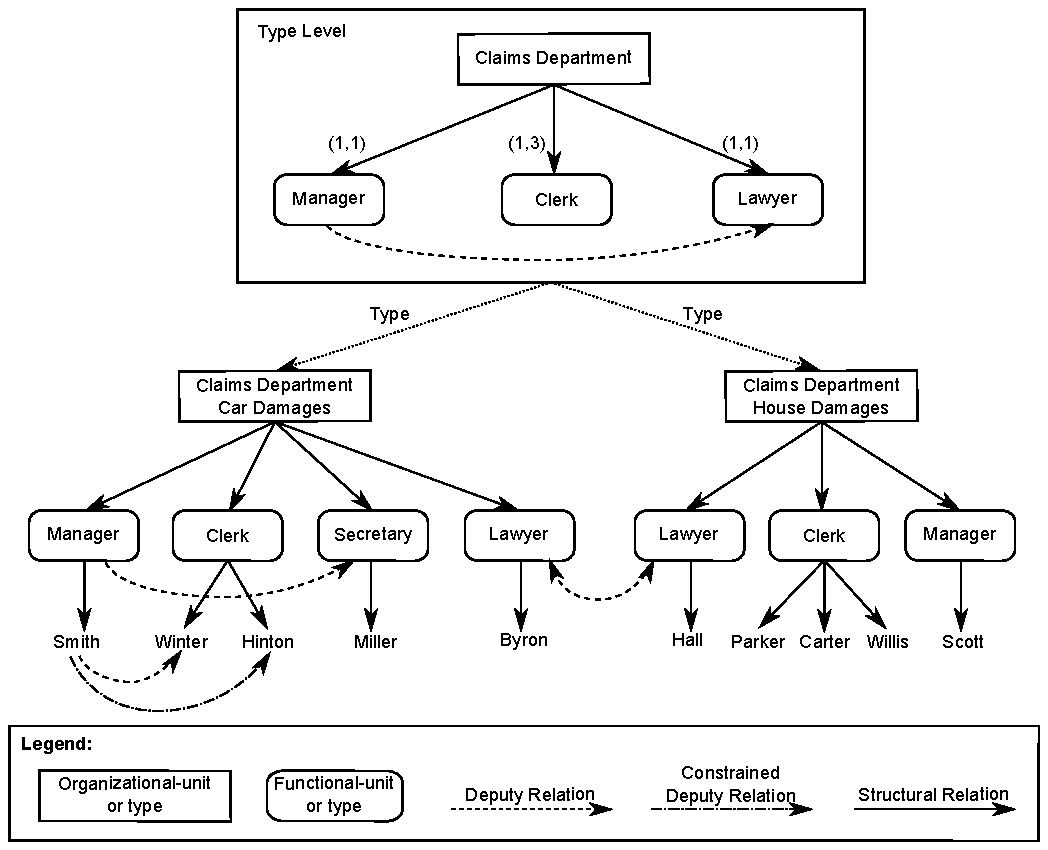
\includegraphics[width=\textwidth]{Figures/alles.pdf}
	\caption{Type and instance level of the example, adapted from \cite[fig. 3]{Lawall2013}}
	\label{Example1}
	\end{figure}

\subparagraph{Lessons Learned}

This section describes additional observations concerning real world organization policies\footnote{A complete overview can be found in \cite{Schaller98}.}.

\subparagraph{Knowledge Hierarchy}
As we have seen there are different levels of organizational knowledge. On the top level general structural assertions like ``a department consists of one to three clerks'' are dominant. We call this level the \emph{type} or \emph{template} level. Knowledge on this level is based on experience and is changed seldom as time goes by. Looking at real world departments -- we will call them \emph{instances} -- things become more concrete and specialized. There are concrete positions and the relationships between them. Finally, actors are assigned to the concrete positions. The organizational structures on this level are changing more frequently according to the demands of the daily business.

\subparagraph{Relationships}
An organization structure is formed by elements and relationships between them. It is important to realize the existence of several relationship types like ``is\_part\_of'', ``is\_deputy'', ``is\_supervisor'', ``reports\_to'' and so on.

Positions are abstractions of persons (actors) having a defined skill set fulfilling specific tasks. These abstractions help defining a more stable model of the organization that is independent from employee turnover. Relationships can be defined between abstract positions or on the concrete actor level.

Relationships are rarely of a general nature. As discussed in our example, relationships depend on specific constraint information like the cash value of a car claim. Even the ``is\_deputy''-relationship can depend on projects or products if you think in the terms of a matrix organization. They can also be only valid for a fixed time period.

\subparagraph{Multidimensional organizations}
Business organizations are multidimensional. Even in organizations that -- at first glance -- are structured hierarchically, there are structures belonging to the so called secondary (``shadow'') organization comprising committees, commissions, boards and so on. The positions and functions of the secondary organization are assigned to the employees. This leads to a multidimensional organization in every case. %We emphasize this point because there are some theories and approaches that are specific to hierarchical structures.

\subsection{Linking the process and the organizational model} \label{chapter_Linking}

Based on the organizational model, a server component is proposed that implements a special architecture and a unique algorithm for the resolution of expressions denoting abstract actors in the sense of subjects. This server is part of a greater system, the IT landscape of the company. ERP, process automation or database management systems can be other components of the landscape. Each of these systems uses mechanisms to map actors to tasks of processes or to permissions on data objects. Instead of maintaining such assignments for each system individually by total enumeration, we propose using an organizational server. This organizational server contains the organizational model. A formal language is used to formulate expressions that define the assignments. Clients send these expressions as requests to the organizational server and retrieve sets of real actors as reply (cf. figure \ref{architecture}). The server offers a versatile interface consisting of only one function \emph{dispatch} that returns a subset of the actors maintained within the organization model.

A major benefit of this approach is that the server forms the result set based on the current organizational model. This means that if actors change functions or relations, these changes have an immediate impact on the client systems. The language expressions remain unaltered. Before the organizational change, ``Manager(*)'' yields (according to fig. \ref{Example1}) the actors Smith and Scott. If Scott leaves the company and is replaced by Willis, the model is changed. Now, the same expression evaluates to Smith and the new manager Willis.

	\begin{figure}[htb!]
	\centering
	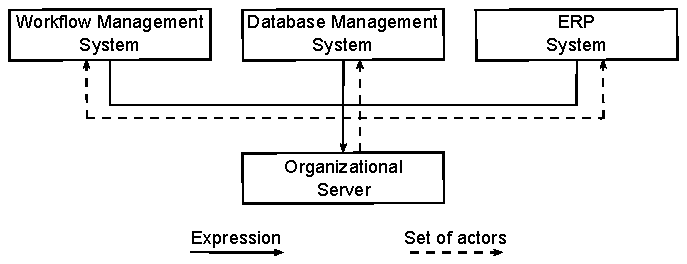
\includegraphics[scale=0.9]{Figures/architecture.pdf}
	\caption{Architecture}
	\label{architecture}
	\end{figure}

An informal overview on the functionality of the proposed server based on the introduced scenario could be assumed as the following. In a process management system a subject is defined by the expression  ``Manager(Claims Department Car Damages)''. At runtime the expression is passed to the organizational server. By traversing the organizational graph in figure \ref{Example1}, the algorithm moves to the department ``Claims Department Car Damages'' looking for a position ``Manager''. After that, the algorithm determines all the actors assigned to that position, finding manager Smith. If Smith is on the job, his identification is handed back to the workflow management system and the search ends. In case that Smith is not available (e.g. through vacation or sickness) the algorithm searches for  deputy relations between Smith and other actors. Obviously, there are two relations. If Winter \textbf{and} Hinton appear in the search result depends on the constraint on the relation to Hinton and whether they are on the job. In case of an empty set, the algorithm moves to the functional-unit manager looking 	for a deputy relation and finds the functional-unit secretary assigned to Miller. If Miller is on the job, her identification will be returned to the workflow management system. If not, the algorithm has the alternative of determining a valid deputy on the type level. Let us assume that the department is linked to the department type as depicted in figure \ref{Example1}. Within this type, the algorithm finds the lawyer as a deputy. It moves back to the instance ``Claims Department Car Damages'' and checks if there is a functional-unit with this name and an actor assigned to that functional-unit that is available. If Byron is on the job, his identification is returned. Otherwise, the lawyer of the ``Claims Department Car Damages'' has a two-way deputy relation with the lawyer of the ``Claims Department House Damages''. If this functional-unit has an actor assigned to itself and the actor is available, the algorithm will hand back his identification (here Hall, the lawyer of the ``Claims Department House Damages''). Otherwise the returned set is empty. In this case, the workflow management system has to postpone the execution of the task.


\section{Formal Specification}

The formalization of the organizational model is described using relations and integrity constraints. In the following we present a simplified model of Schaller's approach.

Within our meta-model an organization is a tuple O = ($name$, $\domaene$, $\OrgElementMenge$, $\relmenge$, $\relationen$) where $name$ denotes the modeled organization. The remaining symbols have the following semantics:

\subsection{Domains $\domaene$}
	$\domaene = \{ \Bezeichner, \zeit, \ID, \relname, \attribute, \WerteMenge, \praedikat \} $ is a set
	of domains consisting of the subsets:

	\begin{itemize}

	\item $\Bezeichner$ an organization specific set of terms describing the building blocks of the
	organization, like "`claims department"', department "`head"' and so on,

	\item $\zeit$ denotes a set of time values, like ``May 19th 2010 08:00:00''.

	\item $\ID$ a set of abstract identifiers.

	\item $\relname$ denotes a set of relationship names, "`deputy"' or "`reports\_to"' for instance.

	\item $\attribute$ a set of attributes used to detail the elements of our model. Attributes are mapped to model elements using the function  $val: \attribute \rightarrow \WerteMenge$ that assigns a value $w \in \WerteMenge$ to each
	$a \in \attribute$.

	\item	$\praedikat$ denotes a set of predicates like "`(ActualYear - HiringYear) $>$ 10"'.

	\end{itemize}

\subsection{Organization Elements $\OrgElementMenge$}
	The set $\OrgElementMenge = \oetyp \cup \ftyp \cup \oe \cup \f \cup \a $ comprises all the building blocks of an organization on the type as well as on the instance level. The elements of $\OrgElementMenge$ represent the nodes of the resulting organization graph.

	\begin{itemize}

	\item $\oetyp$ denotes the set of organizational-unit types, like departments or working groups.


	\item $\ftyp$ is the set of functional-unit types, like the ``manager'', ``lawyers''\ and so on.


	\item $\oe$ represents the set of organizational-units, like departments, committees, teams and so on. As already explained, organizational-units can have a relation to a type. The total function $type_{\oe}: \oe \rightarrow \oetyp \cup NULL$ returns the specific type for every organizational-unit.

	\item $\f$ is the set of functional-units, like positions or roles. There also exists a type function that is almost defined in the same manner as described above. The type of a functional-unit is returned by the function $type_F{\f}: \f \rightarrow \ftyp \cup NULL$.

	$\relstrukturOE_F \subset \oe \times (\oe \cup \f)$ denotes the is\_part\_of-relation between organizational- and functional-units.$\relstrukturOE_F$ on the one hand	describes the mapping of functional-units to organizational-units. On the	other hand the hierarchy between orga-nizational-units can be modeled. When focusing on the organizational-units the relation ${\relstrukturOE_F}^{'} = \relstrukturOE_F \rhd \oe$ has to be irreflexive and cycle-free. ${\relstrukturOE_F}^{''} = \relstrukturOE_F \rhd \f$ has to be surjective.

	\item  $R^{\f}$ denotes a set of user-defined relations. All members $r \in R^{\f}$ have the structure $r \subset (\f \times \f)$ and	are irreflexive.

	\item The set $\a$ denotes the actors: employees (users) and the computer systems. We explicitly model these computer systems because they can carry out tasks and therefore need permissions. $\relstrukturFA \subset \f \times \a$ is a relation and describes the assignments of employees to positions. As seen before, there is also a user-defined set of relationships $R^{\a}$. All relations $r \in R^{\a}$ have the structure $r \subset (\a \times (\a \cup \f))$. Further on, for all $r \in R^{\a}$ the condition $\forall r \in R^{\a}: \left[(x,y) \in r \rightarrow x \neq y \right]$ holds, meaning that every relation	$r \in R^{\a}$ is cycle-free.

	\item Additionally every element of $\OrgElementMenge$ is described as tuple $(id, name)$, with $id \in \ID$ and $name \in \Bezeichner$.

	\end{itemize}

\subsection{Set of Relations $\relmenge$}
	$\relmenge$ denotes a set of relation sets and is defined as
	$\relmenge = \relmengetyp \cup \relmengeinst$, with:

	\begin{itemize}

	\item $\relmengetyp$ denotes the set of relations defined between the types of organizational- and functional-units.
	$\relmengetyp$ is defined as $\relmengetyp = \typstrukturrelation \cup \typbenutzerrelationenmenge$, with:
	\begin{itemize}

		\item $\typstrukturrelation \subset \oetyp \times (\oetyp \cup \ftyp)$ is the ``is\_part\_of''-relation on the type level. Concerning the structure between the elements of $\oetyp$, there are some restrictions. Let's say ${\typstrukturrelation}^{'} = \typstrukturrelation \rhd \oetyp$\footnote{The operator $\rhd$ is defined as $((\rel \subset A \times B) \rhd (C \subset B)) := \{(x,y) \in \rel \, \vert \, y \in C \}$.}.
		An organizational-unit type can not be his own successor. ${\typstrukturrelation}^{'}$ therefore has to be irreflexive and cycle-free.
		Let's have a look at the functional-unit types. Obviously the relationship between $\oetyp$ and $\ftyp$ can be described as ${\typstrukturrelation}^{''} = \typstrukturrelation \rhd \ftyp$. Since organizational-unit types combine functional-unit types, ${\typstrukturrelation}^{''}$ has to be total. On the other side, every $f \in \ftyp$ has to be linked to an organizational-unit type $o \in \oetyp$. ${\typstrukturrelation}^{''}$ therefore has to be surjective.

		\item As explained above, there is the need for a flexible integration of new relation-types into the model. Therefore we define a set of relation-types $\typbenutzerrelationenmenge$. Every relationship $\typbenutzerrelation \in R^{\typsymbol}$ has the structure $\typbenutzerrelation \subset (\ftyp \times \ftyp) \times \praedikat$ and can further be constraint using predicates to restrict the set of valid functional-unit types and therefore the set of valid users\footnote{Please take a look at the relation $\relstrukturFA$ and its according constraints}. Please note that $\typbenutzerrelation$ is used as variable. The relations between the functional-unit types, that can expressed using the term $dom(\typbenutzerrelation)$, are irreflexive. Defining a deputyship between one node and itself is not very meaningful for instance. Concerning the predicates we additionally postulate that each $\typbenutzerrelation \in \typbenutzerrelationenmenge$ has to be a function, assigning each ordered pair $(f,f) \in \ftyp \times \ftyp$ a unique predicate $p \in \praedikat$.

	\end{itemize}
	\item $\relmengeinst$ defines several relations between organizational- and functional-unit types as well as actors. We declare $\relmengeinst$ as 		$\relmengeinst = \relmengeinstOE_F \cup \relmengeinstFA$, with:

		\begin{itemize}

		\item $\relmengeinstOE_F = \relstrukturOE_F \cup \relmengebenutzerinstOE_F$ the set of relations between organizational- and functional-units, with:
			\begin{itemize}
			\item $\relstrukturOE_F \subset \oe \times (\oe \cup \f)$ denotes the ``is\_part\_of''-relation between organiza-tional- and functional-units. On the one hand the relation describes the functional-units belonging to an organizational-unit, on the other hand the organization structure between the units themselves. Let ${\relstrukturOE_F}^{'} = \relstrukturOE_F \rhd \oe$ denote the structure between the organizational-units. According to our description ${\relstrukturOE_F}^{'}$ has to be irreflexive and cycle-free. In the same manner and similar to our definition of ${\typstrukturrelation}^{''}$,${\relstrukturOE_F}^{''} = \relstrukturOE_F \rhd \f$ has to be total and surjective.

			\item $\relmengebenutzerinstOE_F$ is a set of user-defined relations. Every single relation ${\relbenutzerinstOE_F}$ within $\relmengebenutzerinstOE_F$ has the structure ${\relbenutzerinstOE_F} \subset \f \times \f$ and is irreflexive.
			\end{itemize}

		\item $\relmengeinstFA$ denotes a set of relations between functional-units and actors. $\relmengeinstFA$ is defined as $\relmengeinstFA = \relstrukturFA \cup \relmengebenutzerFA$, with:

			\begin{itemize}

			\item $\relstrukturFA \subset \f \times \a$ describes the function assignments of the actors. We demand that every actor is named to at least one function.

			\item $\relmengebenutzerFA$ a set of user-defined, irreflexive relations 	${\relbenutzerFA}$ having the structure $\forall {\relbenutzerFA} \in \relmengebenutzerFA: {\relbenutzerFA} \subset \a \times (\a \cup \f)$. For every $\relbenutzerFA \in \relmengebenutzerFA$ the condition		$\left[(x,y) \in \relbenutzerFA \rightarrow x \neq y \right]$ holds.
			\end{itemize}

		\end{itemize}

	\end{itemize}

	All elements of our model can be detailed using time constraints and attributes.

\subsection{Additional relations $\relationen$}

	$\relationen$ consists of several relations and is defined as $\relationen =\{ \rel_{Time}, \rel_{\attribute},$ $\rel_{Card}, \rel_{val}, \rel_{Name}\}$, with:

	\begin{itemize}
	\item $\rel_{Time} \subset \bigl( \OrgElementMenge \cup \relmenge \bigr)\times \bigl( \zeit \times \zeit \bigr)$ describes the duration of validity of every single organizational element in our model. $\rel_{Time}$ therefore has to be a total relation.

The two functions $start$ and $stop$ denote the birth and death of an organizational element. We define these functions as:
			$$
			\begin{array}{cll}
			start: \bigl( \OrgElementMenge \cup \relmenge \bigr) \rightarrow \zeit, &
				\mbox{with the semantic} & \\
				& start(x \in ( \OrgElementMenge \cup \relmenge ) ) =
				dom( ran ( x \lhd \rel_{Time})) & \\
			stop: \bigl( \OrgElementMenge \cup \relmenge \bigr) \rightarrow \zeit, &
				\mbox{with the semantic} & \\
				& stop(x \in ( \OrgElementMenge \cup \relmenge ) ) =
				ran( ran ( x \lhd \rel_{Time})) & \\
			\end{array}
			$$
It is obvious that the following constraint should hold: $\forall x \in \bigl( \OrgElementMenge \cup \relmenge \bigr): start(x) \leq stop(x)$.  In order to define an existence ad infinitum we introduce the symbol ``$*$''\ concerning the value of the $stop$ function.

	\item $\rel_{\attribute} \subset \bigl( \OrgElementMenge \cup \relmenge \bigr) \times \attribute$ assigns attributes to our organizational elements.
		$\rel_{\attribute}$ is a surjective relation. Thus every attribute can only be assigned to one organizational element.

	\item $\rel_{Card} \subset \typstrukturrelation \times (\natnull \times \natnull)$ assigns cardinalities to our ``is\_part\_of''-relation between organizational- and functional-unit types. $\rel_{Card}$ is a total and unique relation.

		As abbreviations we define the functions $min$ and $max$, with
		$$
		\begin{array}{cl}
		min: \typstrukturrelation \rightarrow \natnull, & \mbox{with the semantic} \\
		& min(r \in \typstrukturrelation) = dom( ran( r \lhd \rel_{Card})) \\
		max: \typstrukturrelation \rightarrow \natnull, & \mbox{with the semantic} \\
		& max(r \in \typstrukturrelation) = ran( ran ( r \lhd \rel_{Card}))
		\end{array}
		$$
		Additionally we demand $\forall r \in \typstrukturrelation: min(r) \leq max(r)$.

	\item Via $\rel_{val} \subset \praedikat \times (\f^{\typsymbol} \cup A)$ each predicate, its typed functional-unit and actors is assigned. The predicate {\em true} holds for all typed functions and actors and we define $\forall x \in \f^{\typsymbol} \cup A: \quad (true, x) \in \rel_{val}$.

	\item $\rel_{Name} \subset \bigl( \typbenutzerrelationenmenge \cup \relmengebenutzerinstOE_F \cup \relmengebenutzerFA \bigr) \times \relname$
		assigns names to our user-defined relations. None of these relations should be nameless. $\rel_{Name}$ therefore has to be total and unique.
		As already mentioned, $\typstrukturrelation, \relstrukturOE_F$ and	$\relstrukturFA$ denote ``is\_part\_of''-relations. A specific naming of these 		relations is therefore unnecessary.
\end{itemize}

\subsection{Policy Resolution}\label{PolicyResolutionFormal}

As discussed in section \ref{chapter_Linking} our organizational server offers an interface with a very small footprint, consisting only of the function "`dispatch"'. The function returns a subset of the actors fulfilling the language expression in conjunction with conditions. These conditions are formulated via the following parameters expected by the function.
\begin{itemize}
	\item a set of organizational-unit names $oe_{bez} \in \Bezeichner$,
	\item a set of tuples consisting of attributes and corresponding values $attr_{oe} \subset (\Bezeichner \times \WerteMenge)$ belonging to defined organizational-units,
	\item a set of functional-unit names $f_{bez} \in \Bezeichner$,
	\item a set of tuples consisting of attributes and corresponding values $attr_{f} \subset (\Bezeichner \times \WerteMenge)$ belonging to functional-units,
	\item a set of actor names $a_{bez} \in \Bezeichner$,
	\item a set of tuples consisting of attributes and related values $attr_{a} \subset (\Bezeichner \times \WerteMenge)$, belonging to actors,
	\item the name of a relation $rel \in \relname$ and
	\item a set of tuples consisting of attributes and corresponding values $attr_{rel} \subset (\Bezeichner \times \WerteMenge)$, belonging to that relation.
\end{itemize}

%The {\tt dispatch}-algorithm works as follows:

	\begin{samepage}
	{\small
	\NumberProgramstrue
	\begin{algorithm}[dispatch]\label{alg:GetIt}
	\begin{program}
	\FUNCT |dispatch|(oe_{bez} \subset \Bezeichner, attr_{oe} \subset (\Bezeichner \times \WerteMenge),
	f_{bez} \subset \Bezeichner, attr_f \subset (\Bezeichner \times \WerteMenge),
	a_{bez} \subset \Bezeichner, attr_a \subset (\Bezeichner \times \WerteMenge),
	rel \in \relname, attr_{rel} \subset (\Bezeichner \times \WerteMenge)) \subset \a
	\BEGIN
	\var \seq{oe \subset \oe; f \subset \f; a \subset A};
	/*|First we have to determine the existing organizational elements|*/
	oe := (\oe \rhd oe_{bez});
	f := (\f \rhd f_{bez});
	a := (A \rhd a_{bez});
	\IF (oe \neq \{\} \vee attr_{oe} \neq \{\}) \label{alg:GetIt:CallGetATbyOE}
	\THEN \RETURN \quad GetATbyOE(oe, attr_{oe}, f, attr_f, rel, attr_{rel})
	\FI
	\IF (f \neq \{\} \vee attr_f \neq \{\})
	\THEN \RETURN \quad GetATbyF(f, attr_f, attr_a, rel, attr_{rel})
	\FI
	\IF (a \neq \{\} \vee attr_a \neq \{\})
	\THEN \RETURN \quad GetAT(a, attr_a, rel, attr_{rel})
	\FI
	\RETURN \{\};
	\END
	\end{program}
	\end{algorithm}
	\NumberProgramsfalse
	}
	\end{samepage}

\noindent The execution of {\tt dispatch(\{Claims Department Car Damages\},\{\},\{Clerk\},\\ \{\},\{\},\{damage sum $<$ \$100\},\{\},\{\})} is equivalent to search all clerks in the organizational-unit {\it car damages} that are authorized to sign claims with a damage sum lower than 100 dollars. The execution will lead to a call of the {\tt GetATbyOE}-function. Based on the values of $oe$, $f$ and $a$ {\tt GetATbyOE} determines the organization elements fulfilling the remaining conditions specified in $attr_{oe}$, $attr_{f}$ and so on.

	%\longpage
	\begin{samepage}
	{\small
	\NumberProgramstrue
	\begin{algorithm}[GetATbyOE]\label{alg:GetATbyOE}
	\begin{program}
	\FUNCT |GetATbyOE|(oe \subset \oe, attr_{oe} \subset (\Bezeichner \times \WerteMenge), f \subset \f,
	attr_{f} \subset (\Bezeichner \times \WerteMenge), rel \in \relname, attr_{rel} \subset (\Bezeichner \times \WerteMenge),
	attr_a \subset (\Bezeichner \times \WerteMenge)) \subset \a
	\BEGIN
	\var \seq{f^{'} \subset \f; oe_{successor},oe_{successor}^{'} \subset \oe;
		o_{p} \subset \oe \times \oe};
	%=====================================================================================
	%\IF attr_{oe} = \{\} \THEN attr_{oe} = \attribute \FI \label{alg:GetATbyOE:kritisch1}
	%=====================================================================================
	/* o_{p}| denotes the vector corresponding to oe|*/;
	o_{p} := \{(x,y) \vert x \in oe \wedge y \in \oe \};\label{alg:GetATbyOE:Vektor}
	oe_{successor} := dom \left( \left({\left({\left({\relstrukturOE_F}^{'}\right)}^{*}\right)}^{T}\right) \circ o_{p} \right);\label{alg:GetATbyOE:Nachfolger}
	\IF (oe_{successor} = \{\})
	\THEN oe_{successor} := \oe; \label{alg:GetATbyOE:kritisch2}
	\FI
	%=======================================================================================
	%oe_{Nachfolger}^{'} := dom( \{ oe_{Nachfolger} \} \lhd \rel_{\attribute} \rhd attr_{oe} )
	%=======================================================================================
	oe_{successor}^{'} := GetOrgElements( oe_{successor}, attr_{oe});
	\IF (f = \{\})\label{alg:GetATbyOE:fIstNull}
	\THEN
		/*|determine all functional-units of the organizational-units|*/
		f^{'} := ran ( \{oe_{successor}^{'}\} \lhd \relstrukturOE_F ) \cap F;
		\RETURN \quad |GetATbyF|(f^{'}, attr_{f}, attr_a, rel, attr_{rel});
	\ELSE \label{alg:GetATbyOE:fIstNichtNull}
		/*|which of the preselected functional-units belong to|*/
		/*|the organizational-units determined in |oe_{successor}^{'}?*/
		f^{'} := ran ( \{oe_{successor}^{'}\} \lhd \relstrukturOE_F \rhd \{f\}) \cap F;
		\RETURN \quad |GetATbyF|(f^{'}, attr_{f}, attr_a, rel, attr_{rel});
	\FI
	\RETURN \quad \{\};
	\END
	\end{program}
	\end{algorithm}
	\NumberProgramsfalse
	}
	\end{samepage}

\noindent Line \ref{alg:GetATbyOE:Vektor} describes the declaration of a relational vector. The calculation of all successors in line \ref{alg:GetATbyOE:Nachfolger} is obtained by multiplying the transpose of the irreflexive closure of ${\relstrukturOE_F}^{'}$ with our vector $o_{p}$. After that we select the appropriate organizational-units.\\

In the case of the functional-unit set $f$ passed to our function is empty, the algorithm selects all functional-units of the calculated transitive-reflexive closure and calls the function {\tt GetATbyF} (line \ref{alg:GetATbyOE:fIstNull}). If $f$ != $\{\}$ the relevant functional-units are selected in dependency on the specified organizational-units. After that the function {\tt GetATbyF} is called	(line \ref{alg:GetATbyOE:fIstNichtNull}).

	%\longpage
	\begin{samepage}
	{\small
	\NumberProgramstrue
	\begin{algorithm}[GetATbyF]\label{alg:GetATbyF}
	\begin{program}
	\FUNCT |GetATbyF|(f \subset \f, attr_f \subset (\Bezeichner \times \WerteMenge), attr_a \subset (\Bezeichner \times \WerteMenge),
	rel \in \relname, attr_{rel} \subset (\Bezeichner \times \WerteMenge)) \subset \a
	\BEGIN
	\var \seq{f^{'},f^{''} \subset \f; a \subset A};
	\IF (attr_f = \{\})
	\THEN attr_f := \attribute;
	\FI
	f^{'} := f;
	\IF (f^{'} = \{\})
	\THEN f^{'} := \f;
	\FI
	%==========================================================
	%f^{'} := dom ( \{f\} \lhd \rel_{\attribute} \rhd attr_f );
	%==========================================================
	f^{''} := GetOrgElements( f^{'}, attr_f );
	a := ran( f^{''} \lhd \relstrukturFA );
	\RETURN \quad |GetAT|(a, attr_a, rel, attr_{rel});
	\END
	\end{program}
	\end{algorithm}
	\NumberProgramsfalse
	}
	\end{samepage}

\noindent Function {\tt GetATbyF} determines the set of functional-units fulfilling the attributes passed over as parameters first. After that corresponding actors are selected and handed over to {\tt GetAT}.\\

Algorithm \ref{alg:GetAT} describes the core idea of our system. The passed parameters are being processed from the actor level up to level of organizational- and functional-unit types. Individual rules therefore have a higher priority than policies specified on the more abstract type level.

	{\small
	\NumberProgramstrue
	\begin{algorithm}[GetAT]\label{alg:GetAT}
	\begin{program}
	\FUNCT |GetAT|(a \subset \a, attr_a \subset (\Bezeichner \times \WerteMenge), rel \in \relname, attr_{rel} \subset (\Bezeichner \times \WerteMenge)) \subset \a
	\BEGIN
	\IF (attr_a = rel = attr_{rel} = \{\})\label{alg:GetAT:trivial}
	\THEN \RETURN \quad a;
	\FI
	/* |exit for recursions| */
	\IF (attr_a \neq \{\} \wedge (rel = attr_{rel} = \{\})) \label{alg:GetAT:Aussprung}
	\THEN
		\IF a = \{\} \THEN a := \a \FI \label{alg:GetAT:A-Erweiterung}
		%=======================================================================================
		%a := dom \bigl( \{a\} \lhd \rel_{\attribute} \rhd \{attr_a\} \bigr); \label{alg:GetAT:1}
		%=======================================================================================
		\RETURN \quad  GetOrgElements( a, attr_a ); \label{alg:GetAT:1}
	\FI
	\IF rel \neq \{\} \label{alg:GetAT:komplex}
	\THEN
		\IF a = \{\} \THEN a := \a \FI
		%=======================================================================================
		%\IF attr_{rel} = \{\} \THEN attr_{rel} := \attribute \FI
		%=======================================================================================
		\var \seq{\rel_x, \rel_x^{'} \in \relmengebenutzerFA; y \subset (\f \cup \a)};
		/* | is there a user-defined relation fulfilling the attributes?|*/
		%\rel_x^{'} := name^{-1}(rel) \cap \relmengebenutzerFA; \label{alg:GetAT:FA}
		\rel_x^{'} := dom(\rel_{Name} \rhd rel) \cap \relmengebenutzerFA; \label{alg:GetAT:FA}
		%=======================================================================================
		%\rel_x := dom(\{\rel_x^{'}\} \lhd \rel_{\attribute} \rhd attr_{rel});
		%=======================================================================================
		\rel_x := GetOrgElements( \rel_x^{'}, attr_{rel});
		\IF \rel_x \neq \{\}
		\THEN
		%=======================================================================================
		%	z := ran ( dom ( (\{a\} \lhd \rel_x) \lhd \rel_{\attribute} \rhd \{attr_{rel}\} ) );
		%=======================================================================================
			\var \seq{z \subset A \cup \f; w,y \subset A};
			z := ran( GetOrgElements(\{a\} \lhd \rel_x, attr_{rel}) );
			/*| select the actors according to |$z$
			w := z \cap \a;
			/*| select the actors according to | \relstrukturFA */
			y := ran (\{ \{z\} \cap \f\} \lhd \relstrukturFA);
			\RETURN \quad w \cup y;
		\ELSE
			\var \seq{\rel_x^\f, {\rel_x^\f}^{'} \subset \relmengebenutzerinstOE_F};
			%{\rel_x^\f}^{'} := name^{-1}(rel) \cap \relmengebenutzerinstOE_F; \label{alg:GetAT:FF}
			{\rel_x^\f}^{'} := dom(\rel_{Name} \rhd rel) \cap \relmengebenutzerinstOE_F; \label{alg:GetAT:FF}
			%===================================================================================
			%\rel_x^\f := dom(\{{\rel_x^\f}^{'}\} \lhd \rel_{\attribute} \rhd attr_{rel});
			%===================================================================================
			\rel_x^\f := GetOrgElements({\rel_x^\f}^{'}, attr_{rel});
			\IF \rel_x^\f \neq \{\}
			\THEN
				\var \seq{a^{'} \subset A};
				/*|select all actors connected to the functional-unit |*/
				a^{'} := ran \left( \{ ran \left( \rel_x^\f \right) \} \lhd \relstrukturFA \right);
				\RETURN \quad |GetAT|(a^{'}, attr_a, \{\},\{\});
			\ELSE /*|lookup in the  type level|*/
			\var \seq{\rel_x^\ftyp,{\rel_x^\ftyp}^{'} \subset \typbenutzerrelationenmenge};
			%{\rel_x^\ftyp}^{'} := name^{-1}(rel) \cap \typbenutzerrelationenmenge; \label{alg:GetAT:FtFt}
			{\rel_x^\ftyp}^{'} := dom(\rel_{Name} \rhd rel) \cap \typbenutzerrelationenmenge; \label{alg:GetAT:FtFt}
			%===================================================================================
			%\rel_x^\ftyp := dom(\{{\rel_x^\ftyp}^{'}\} \lhd \rel_{\attribute} \rhd attr_{rel});
			%===================================================================================
			\rel_x^\ftyp := GetOrgElements({\rel_x^\ftyp}^{'}, attr_{rel});
			\IF \rel_x^\ftyp \neq \{\}
			\THEN
				\var \seq{f^{'},f^{''} \subset \f; a^{'},a^{''},a^{'''} \subset A};
				/*|1. address all true relationships |*/ \label{alg:GetAT:PraedikateStart} \label{alg:GetAT:WahrePraedikate}
				%/*|mit dem Pr"adikat "`wahr"'|*/
				f^{'} := dom \bigl( type_F^{\typsymbol} \rhd ran( dom (\rel_x^\ftyp \rhd \{wahr\}))\bigr);
				a^{'} := ran \bigl( f^{'} \lhd \relstrukturFA \bigr);
				/*|2. address false relationships |*/\label{alg:GetAT:NichtWahrePraedikate}
				%/*|Pr"adikaten ungleich "`wahr"'|*/
%				/* */
				/*|2.1 address typed functional-units |*/
				f^{''} := dom \bigl( \bigl( type_F^{\typsymbol} \rhd ran( dom (\rel_x^\ftyp \rrhd wahr\})) \bigr)
				\cap
				ran \bigl( ran(\rel_x^\ftyp \rrhd \{wahr\}) \lhd \rel_{val} \bigr) \bigr);
				a^{''} := f^{''} \lhd \relstrukturFA;
				/*|2.2 address direct relationships|*/
			a^{'''} :=
				\bigl( dom \bigl( type_F^{\typsymbol} \rhd ran( dom (\rel_x^\ftyp \rrhd \{wahr\})) \lhd \relstrukturFA \bigr)
				  \cap ran \bigl(  ran(\rel_x^\ftyp \rrhd \{wahr\}) \lhd \rel_{val} \bigr) \bigr);
				\RETURN \quad |GetAT|(a^{'} \cup a^{''} \cup a^{'''}, attr_a, \{\},\{\}); \label{alg:GetAT:PraedikateStop}
			\ELSE
				/*| no corresponding relationship found |*/

				\RETURN \quad \{\};
			\FI
		\FI
	\FI
	\FI
	\END
	\end{program}
	\end{algorithm}
	\NumberProgramsfalse
	}

\noindent Line \ref{alg:GetAT:trivial} describes the trivial case. If the only parameter is a set of actors the return value will be the same set.\\

In case that attributes are handed over (that have to be fulfilled by the respective actors) and no user-defined relation was defined (line~\ref{alg:GetAT:Aussprung}), the algorithm determines all actors with a fulfilling attribute set. If $a$ is empty, all actors (line \ref{alg:GetAT:A-Erweiterung}) are used within the search (line \ref{alg:GetAT:1}). \\

The core concept of the algorithm starts with line \ref{alg:GetAT:komplex}. The following user-defined relations have to be resolved:
\begin{itemize}
	\item The relation between actors and functional-units ($\relmengebenutzerFA$),
	\item The relation between functional-units ($\relmengebenutzerinstOE_F$) and
	\item The relation between functional-unit types ($\typbenutzerrelationenmenge$)
\end{itemize}

If no corresponding relation on the actor level can be found (line \ref{alg:GetAT:komplex}), the algorithm checks for a connection between two functional-units ($\relmengebenutzerinstOE_F$) in order to retrieve the attached actors. If no match is possible, the algorithm searches for a relation on the more abstract type level (line \ref{alg:GetAT:FtFt}). If a relation can be found these policies are used for retrieving matching actors on the instance level. Lines \ref{alg:GetAT:PraedikateStart} to \ref{alg:GetAT:PraedikateStop} show the semantics of the predicates $p \in \praedikat$ of the relation $\typbenutzerrelation \in \typbenutzerrelationenmenge$. All not predicate constrained relations are evaluated (line \ref{alg:GetAT:WahrePraedikate}), first. After that the algorithm examines the constrained relations (line \ref{alg:GetAT:NichtWahrePraedikate}).  The resulting actor set is used for a recursive call of algorithm \ref{alg:GetAT}.\\

\noindent Algorithm {\tt GetOrgElements} selects those elements fulfilling a defined attribute set $attr$ from the set of organizational-units and relations.

	%\longpage
	\begin{samepage}
	{\small
	\NumberProgramstrue
	\begin{algorithm}[GetOrgElements]\label{alg:GetOrgElements}
	\begin{program}
	\FUNCT |GetOrgElements|(k \subset \OrgElementMenge \cup \relationen, attr \subset (\Bezeichner \times \WerteMenge)) \subset \OrgElementMenge \cup \relationen
	\BEGIN
	\var \seq{ x \subset \OrgElementMenge \cup \relationen};
	x := \{\};
	\FOREACH y \in k~\DO
		\IF CheckAttributes(y, attr)
		\THEN
			x := x \cup y;
		\FI
	\OD
	\RETURN \quad x;
	\END
	\end{program}
	\end{algorithm}
	\NumberProgramsfalse
	}
	\end{samepage}

\noindent The following algorithm checks if an attribute of set $attr$ is mapped to an organizational element or relation $k \in \OrgElementMenge \cup \relationen$.

	\begin{samepage}
	{\small
	\NumberProgramstrue
	\begin{algorithm}[CheckAttributes]\label{alg:CheckAttributes}
	\begin{program}
	\FUNCT |CheckAttributes|(k \in \OrgElementMenge \cup \relationen, attr \subset (\Bezeichner \times \WerteMenge)) \subset \boole
	\BEGIN
	\var \seq{attr_k \subset \attribute};
	\IF (attr = \{ \})
		\THEN \RETURN \quad \true;
	\ELSE
		attr_k := ran( k \lhd \rel_{\attribute});
		\IF ( dom(attr) \subset ran( attr_k ))
		\THEN
			\FOREACH y \in attr~\DO
				\IF (ran(y) \neq val(attr_k \rhd dom(y)))
				\THEN \RETURN \quad \false;
				\FI
			\OD
			\RETURN \quad \true;
		\ELSE \RETURN \quad \false;
		\FI
	\FI
	\END
	\end{program}
	\end{algorithm}
	\NumberProgramsfalse
	}
	\end{samepage}

\noindent If the required attributes and attribute values are mapped to an organizational element or relation, function {\tt CheckAttributes} returns $true \in \boole$, or otherwise $false \in \boole$. $\boole = \{ true, false \}$ denotes the set of boolean values.

\section{Implementation}
The formalism discussed in this contribution is implemented in a prototype. Figure \ref{proto-gui} depicts part of this implementation -- the graphical user interface (GUI). It contains a \emph{model} editor, a \emph{search} area, a \emph{tree-navigation} as well as an \emph{attribute pane} and a \emph{relation list} for a selected organizational element.

\begin{figure}
\centering
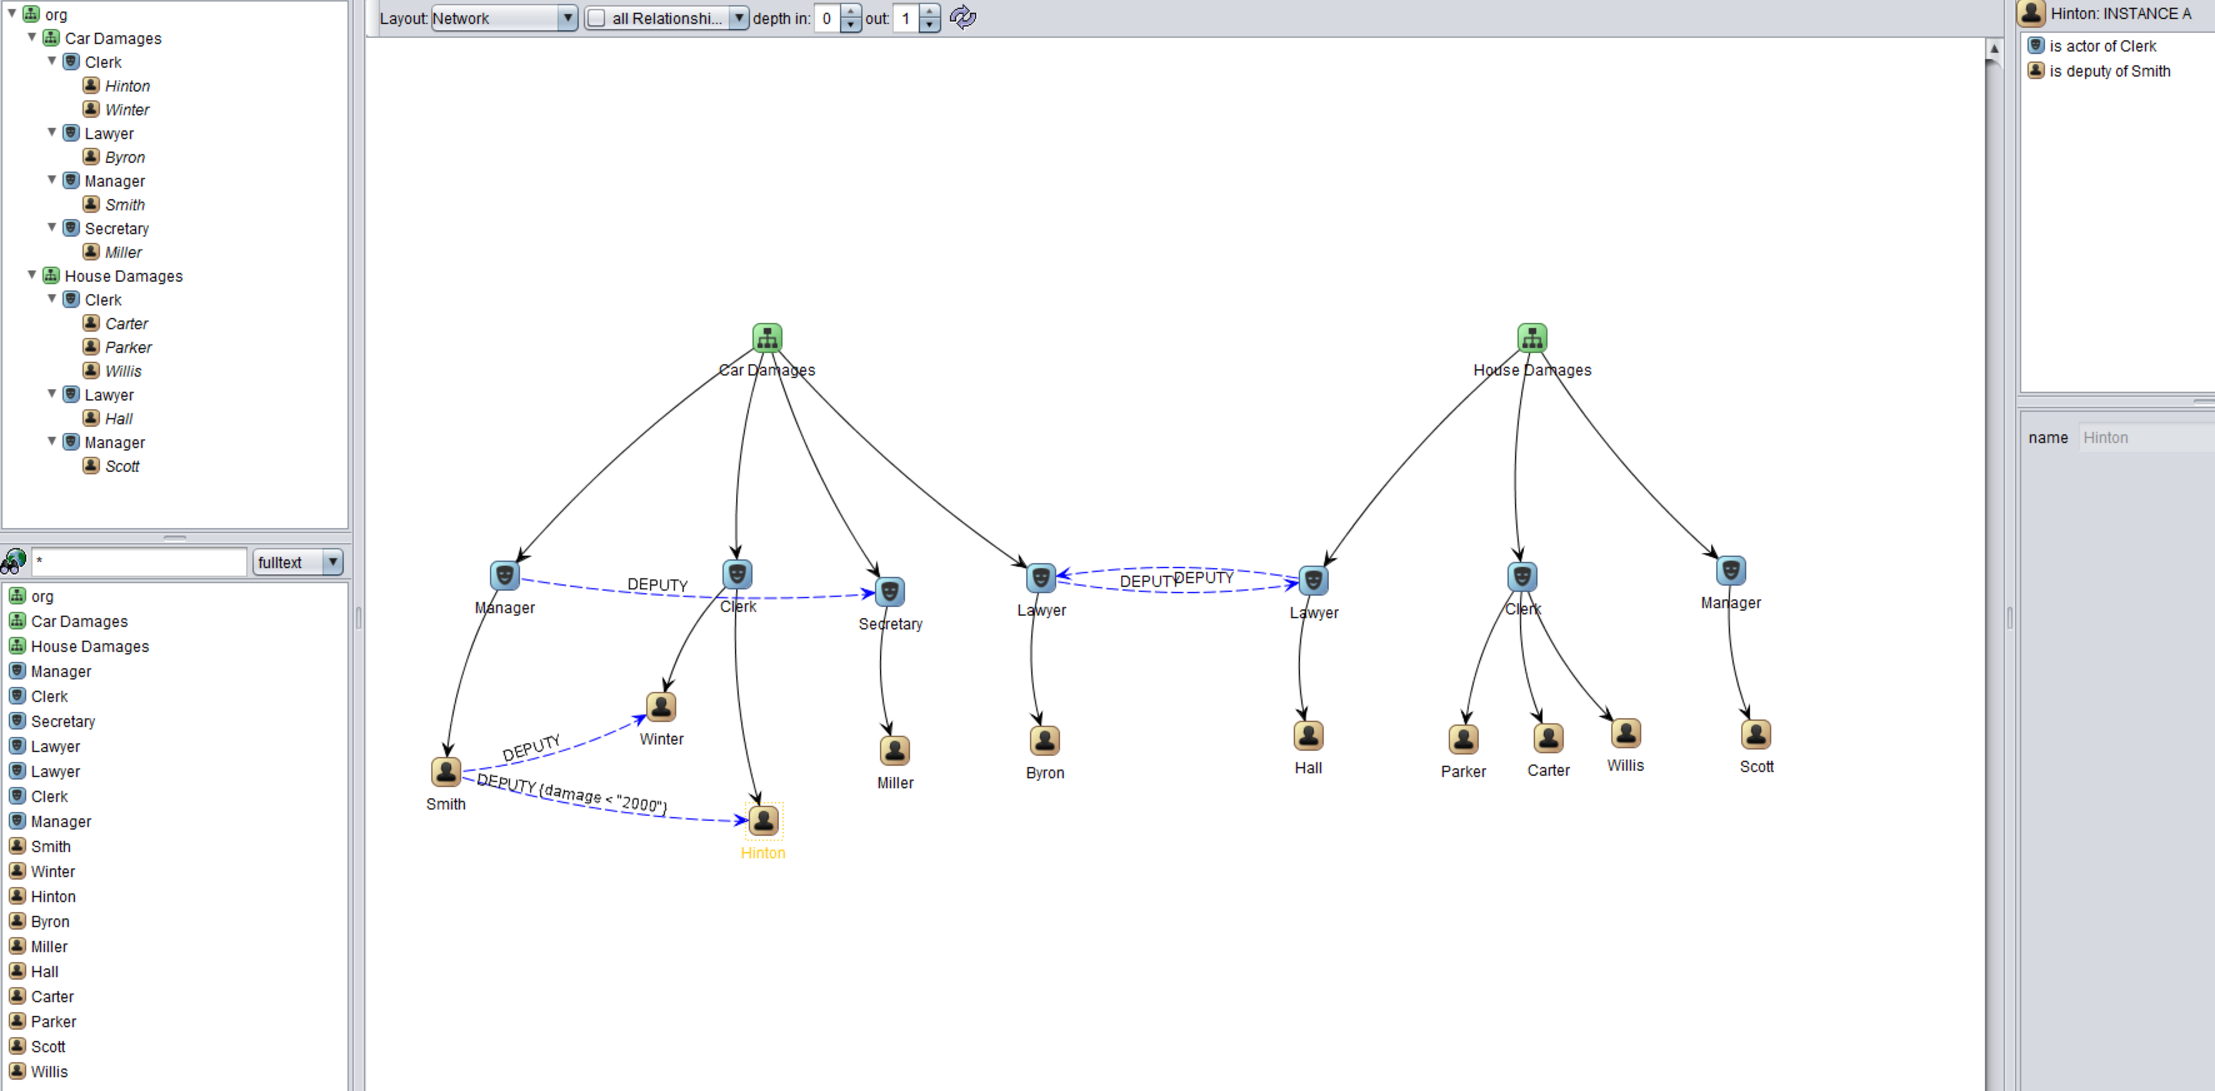
\includegraphics[width=\textwidth]{Figures/corg}
\caption{Screenshot: Implementation of the $\mathcal{C-ORG}$} GUI
\label{proto-gui}
\end{figure}

\begin{description}
  \item[The \emph{model editor}] provides a graph-based view on the organizational structure. Organizational elements are represented as nodes and their relations as edges. It provides means to navigate the model by centering on selected nodes. As the central component of the user interface, it is discussed below in more detail.
	\item[The \emph{search area}] can be used to retrieve a list of organizational elements. It has two modes of operation:
	  \begin{enumerate}
		  \item It provides a simple text index search for attribute values, e.g. entering ``Wi*'' will yield Winter and Willis.
			\item It can also be used to evaluate language expressions based on the approach described in sections \ref{Chapter_PolicyResolution} and \ref{PolicyResolutionFormal}. An expression is entered and the result set for the current state of the organizational model is shown.
		\end{enumerate}
	\item[The \emph{tree-navigation}] projects the concrete organizational structure on a tree. Consequently, entities are duplicated in the projection if they can be reached on different paths.
	\item[The \emph{attribute pane}] in the bottom right section shows the attributes of the currently selected node or relation. It allows a quick modification, e.g. the assignment of a predicate to a relation.
	\item[The \emph{relation list}] lists all relations of the currently selected node, independent from the relation-types hidden in the model editor. This allows access to connected nodes and significantly reduces the time required to alter existing relations.
\end{description}

For quick access, elements can be dragged from any of the outer GUI sections and dropped into the model editor. If the elements have existing relations to the nodes already shown in the model editor, these relations will be shown as well. Otherwise, the elements are represented as unconnected nodes.

\begin{figure}
\centering
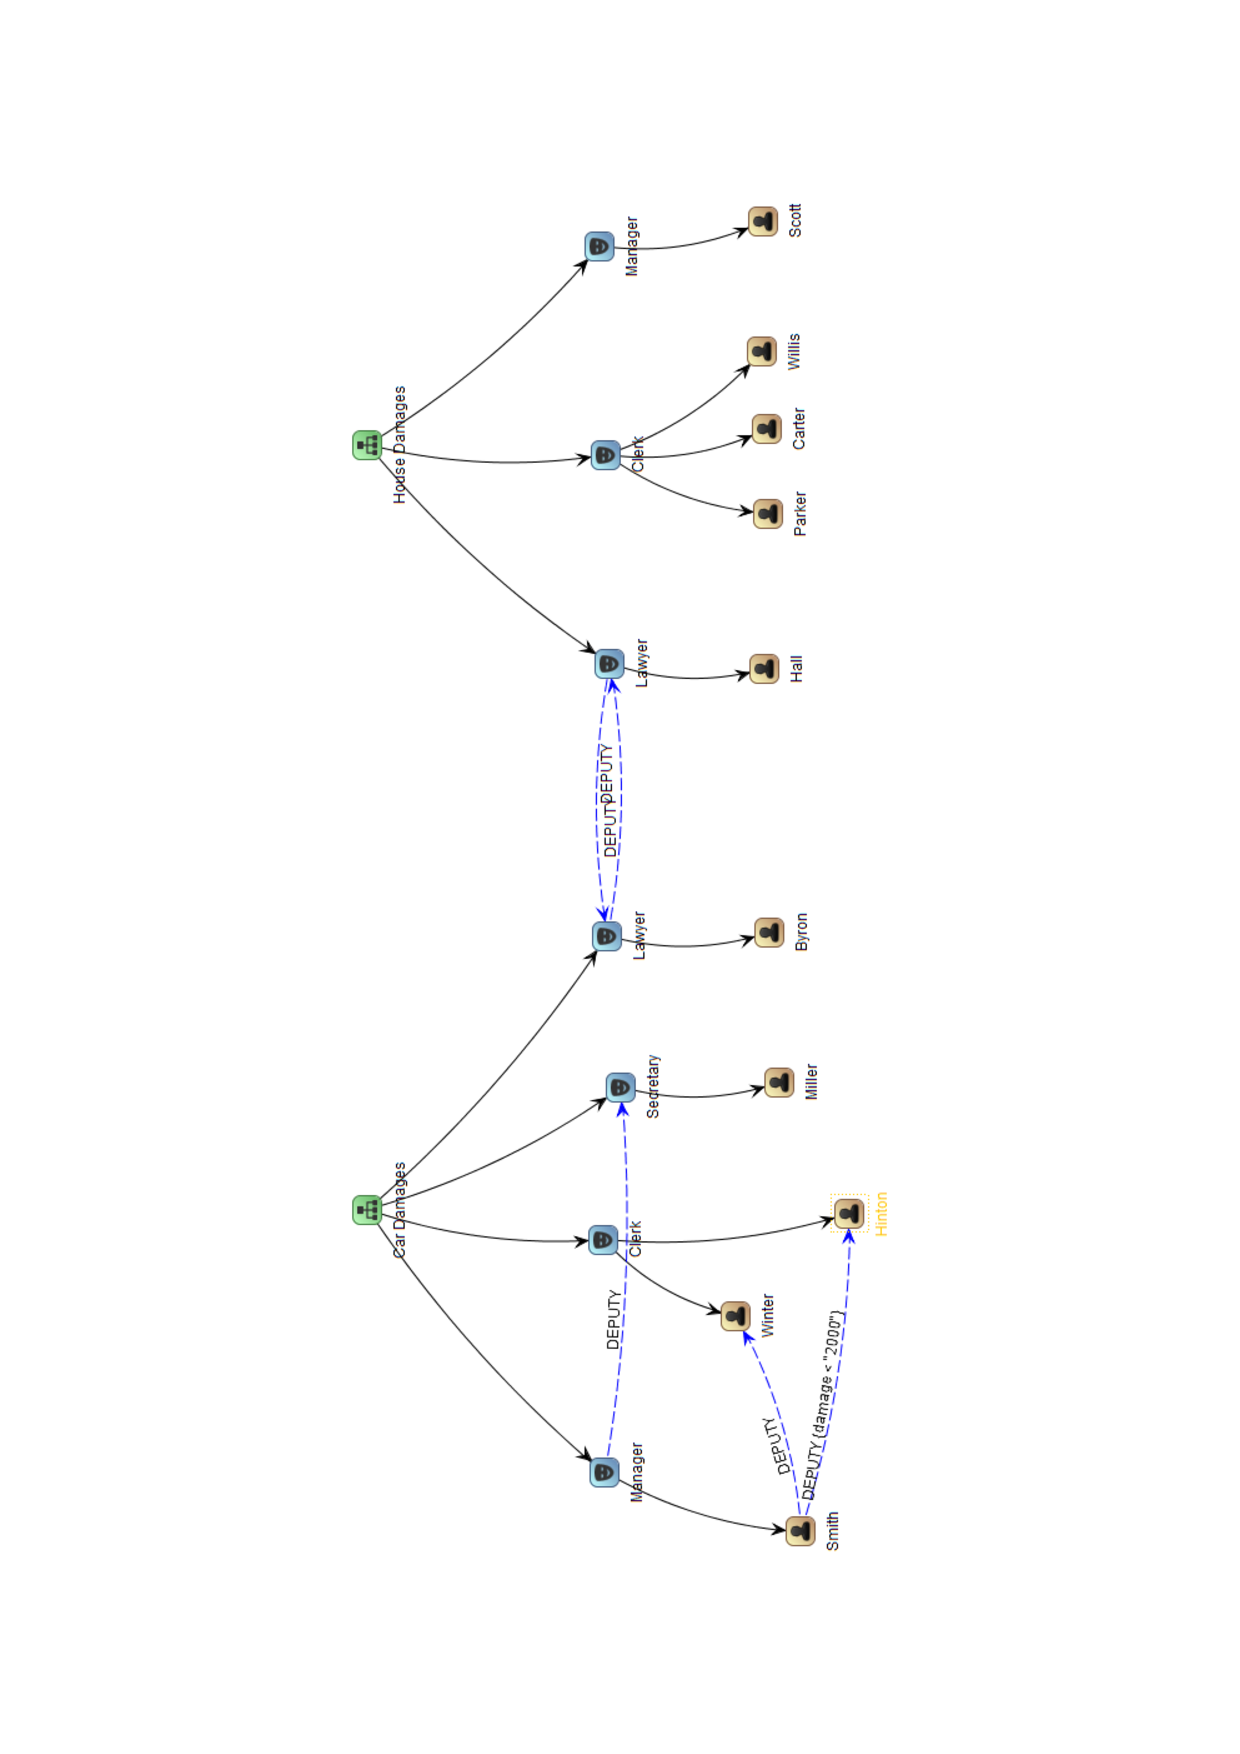
\includegraphics[width=\textwidth]{Figures/corg-graph.pdf}
\caption{Model Region of the Implementation}
\label{proto-model}
\end{figure}

Figure \ref{proto-model} provides an enlarged view of the model editor\footnote{It shows the example model (cf. fig. \ref{Example1}). The type level is hidden.}.
Users perform most modifications of the organizational model via this component.
In addition to navigating the model, they can create, modify and delete organizational elements and their interconnections.

It contains the model with the desired\footnote{The relation-types to be shown can be selected.} relations. The editor also shows concrete constraints (predicates) on relations, e.g. the deputy relation with \emph{damage $<$ ``2000''} between \emph{Smith} and \emph{Hinton}.


In addition to the user interface, the implementation provides a service that can accept language expressions from client systems. This interface is based on the Representational State Transfer (REST) paradigm.



\section{Physical infrastructure}

\todo{Bibtex-File muss noch angepasst werden.}

The previous remarks always referred to human actors. But executors in a business process can also be machines or software components. We will therefore look at how the concept presented in the previous chapters can be extended to the area of non-human actors. Here, the already introduced concepts such as substitutions are also used. 

Let us take a look at the Industry 4.0 area. 

Production plants as we know them today are actually overthought within the smart factories initiative. Central production plans for manufacturing big numbers of similar products are replaced by intelligent objects embedded in self-organizing systems called smart factories \cite{Gronau2015}. These objects are cyber-physical systems \cite{meissner2013} using intelligent sensors for gathering information about the world around them.  They are able to react to environmental changes and to generate plans for fulfilling their goals. So, if a customer orders a product at a manufacturing company an agent responsible for the production of the article is created. This agent knows all about the bill of material and the working plan for the creation of the product. On basis of this information the agent generates a plan how the product can be manufactured. For this he has to talk other agents representing the resources of the company. 

%In this article we show a graph-based approach for maintaining the resources of a smart factory and searching for them using a declarative query language. This language can be used by the production agent looking for resources that are able to fulfill manufacturing tasks of the working plan.

%\subsection{Organizational Model} \label{modell} 

\begin{figure*}[htb!]
	\centering
	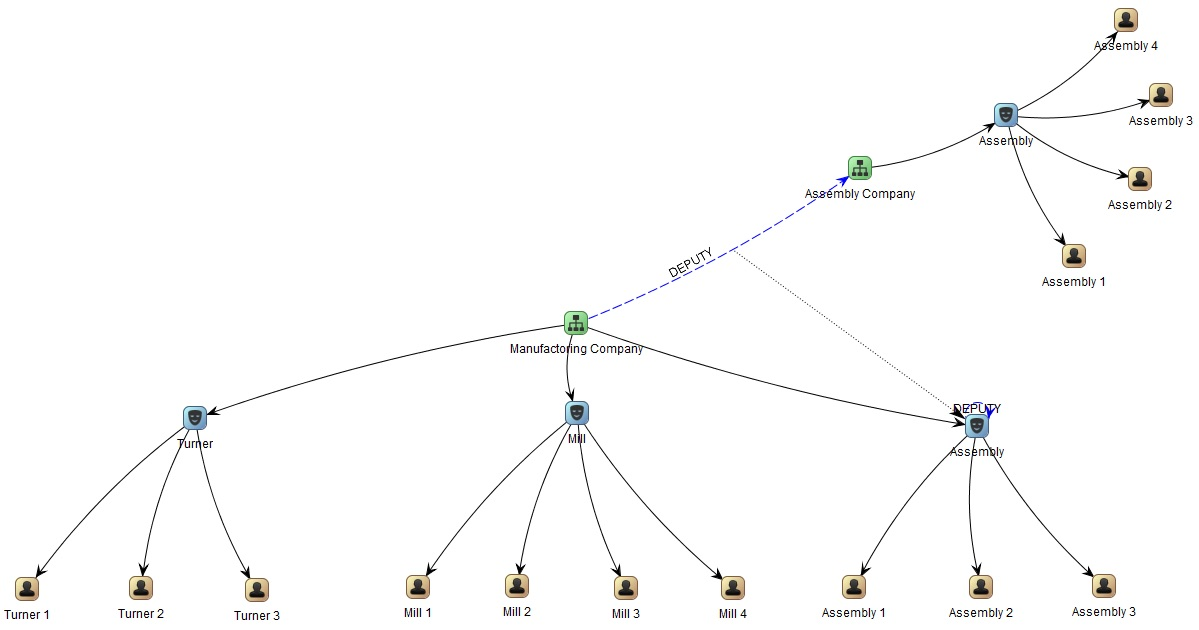
\includegraphics[width=\textwidth]{Figures/orgamodelfed.jpg}
	\caption{Federation between Partner Companies}
	\label{fig:federation}
\end{figure*}

Figure \ref{fig:federation} depicts an excerpt of the organizational model of a manufacturing company producing wooden chairs. The model encompasses the internal organizational unit \emph{Manufacturing Company} with the subordinate internal functional units \emph{Turner}, \emph{Mill} and \emph{Assembly}. The internal resources \emph{Turner 1} to \emph{Turner 3} are related to \emph{Turner}, \emph{Mill 1} to \emph{Mill 4} belong to \emph{Mill} and \emph{Assembly 1} to \emph{Assembly 4} are part of the internal functional unit \emph{Assembly}. 

The properties and capabilities of the elements of the organization can be described using attributes. In our example, the maximum length of a workpiece to be processed and the shape of a workpiece on the machines is of interest.
Table \ref{tab:intagents}  describes an excerpt of attributes in conjunction with their values. 

%The table \ref{tab:intagents} depicts attribute-value pairs of internal automatic resources of the \emph{Manufacturing Company}.
\begin{table}[htb!]
	\centering
	\begin{tabular}{|l||l|l|}
		\hline
		Resource & Attribute & Value \\ 
		\hline
		\hline
		Turner 1 & minworkpieceLength & 30 \\
		\hline 
		& maxworkpieceLength & 50\\
		\hline
		& workpieceKind & octagonal\\
		\hline
		&...&...\\
		\hline
		Turner 2 & minworkpieceLength & 35\\
		\hline
		& maxworkpieceLength & 40\\
		\hline
		& workpieceKind & octagonal\\
		\hline
		&...&...\\
		\hline
		Turner 3&minworkpieceLength & 40 \\
		\hline
		& maxworkpieceLength & 50\\
		\hline
		& workpieceKind & square\\
		\hline		
		&...&...\\
		\hline
		Mill 1& maxLength & 100cm \\
		\hline
		& maxWidth & 100cm\\
		\hline
		& maxHeight & 20 cm\\
		\hline
		Mill 2& .... & ... \\
		\hline
		Assembly1 & Type & 304456\\
		\hline
		& ... & ...\\
		\hline
		Assembly2(PC) & Type & 304456\\
		\hline
		& ... & ...\\
		\hline
	%	&...&...\\
	%	\hline
	%	Mill 3& & \\
	%	\hline
	%	&...&...\\
	%	\hline
	%	Mill 4& & \\
	%	\hline
	%	&...&...\\
	%	\hline
	%	Assembly 1& & \\
	%	\hline
	%	&...&...\\
	%	\hline
	%	Assembly 2& & \\
	%	\hline
	%	&...&...\\
	%	\hline
	%	Assembly 3& & \\
	%	\hline
	%	&...&...\\
	%	\hline
	\end{tabular} 
	\caption{Attributes of Resources} 
	\label{tab:intagents}
\end{table}

Looking at the relationships there exists an external partner company (assembly company) that can take over assembly tasks on load peaks
\footnote{The automated propagation of model elements (entities, relations and attributes) to partner organizations is described in \cite{Lawall2014a}.}. The federation between the manufacturing company and the assembly company extends the aforementioned organizational model. The external organizational unit \emph{Assembly Company} encompasses the external functional unit \emph{Assembly} in conjunction with the external resources \emph{Assembly 1} to \emph{Assembly 4}. 

%So a partner company can act as a proxy. This substitution is described in detail using attributes and hyperedges. For a deeper understanding, please refer to the article \cite{Lawall2014a}.  

Finding the correct agent for a specific task is done by resolving an organzational language expression that is defined in the subject specification.
The expression can reference entities, relations and/or attributes. 
Suppose a production agent wants to have 64 chair legs manufactured for the production of a batch of chairs of type 304456. He first looks in the master data record to see what specifications the legs must have. He finds a length of 40 cm and octagonal shape. He can use these two specifications to find a suitable machine. The expression looks like this:\\

\texttt{(Turner)(Manufacturing Company). ATT.(minworkpieceLength $\leq$ "40" AND maxworkpieceLength $\geq$ AND workpieceKind = "octagonal")}\\

This means the production agent is looking for an agent of type "`turner"' that is able to produce workpieces with length 40cm and an octogonal form.The
search is local to the manufacturing company. In our example, turning machines 1 and 2 are eligible for the production step.
Finding a production resource to manufacture the 64 seats and backrests works on the same principle. Now the chairs still have to be assembled. The agent finds a suitable assembly unit with the following query:\\

\texttt{ (Assembly)(*).ATT.\\(Model $=$ "304456"))} \\
 
The asterisk means that substitutions are also permitted for this request. Thus, the company's own production facility (Assembly 1) as well as the machine of the partner company (Assembly 2) can be found. Depending on the degree of workload of the resources, the agent decides whether he then locks the order on his own machine or the machine of the partner company. \\

Similar to production resources, software products, actuators or sensors can be modelled and managed according to the same principle. 


%\section{IT-Systems and Software}

% Review Christian Stary January 2020

\chapter{Aspects for further standardisation activities}

CS: Hochkommas und - im pdf falsch gedruckt.

In this chapterr various aspects of the subject oriented modelling and programming concept are outlined. These aspects have already been published on different conferences. The following sections are based on these publications. CS: They contain original text parts and thus, the conclusions need to be aligned to the standardization effor, as tried for Fog Computing.
The concepts described in theses sections will be part of future standardisation activities.
The following sections are based on following publications:\\
\begin{list}{-}
	\item Subjects and Shared Input Pools:
	\item Hierarchies in Communication Oriented Business Process Models:
	\item Business Activity Monitoring for S-BPM: \cite{article:SubProcessMon}
	\item Subject Oriented Project Management:
	\item Subject-oriented Fog Computing: \cite{article:FogComp}
	\item Activity based Costing \cite{article:SBPMCosting}
\end{list}

\section{Subjects and Shared Input Pools}

Shared input pools have the same structure like subject-specific ones, and thus, the same properties like the standard input pool. The only difference is that different subjects can deposit in or remove messages from a shared input pool. Subjects that want to send a message via a shared input pool do not use a subject name as addressee of a message, but the name of a shared input pool instead. In a distributed system several shared input pools for different purposes can be used. Figure 7 shows the slightly changed structure of the traffic management system when operating it with a shared input pool CS: hier fehlt das originäre Beispiel als Bezugspunkt. The subject "Car detection" represents the shared input pool.


\begin{figure}[htbp]
	\centering
	\includegraphics[width=0.7\linewidth]{Figures/Chapter5/figuresshared/SharedInputPoolExample.jpg}
	\caption[Traffic Management System with Shared Input Pool]{Traffic Management System with Shared Input Pool}
	\label{fig:SharedInputPooTraffic}
\end{figure}


Shared input pools make a distributed system more flexible when additional participants or nodes are added. For instance, a third intersection control could be added to the traffic management system without much effort. In this case, only the additional detectors and the components for controlling the intersection have to be complemented and linked to the shared input pool. The extension would have no impact on the behavior of the other subjects and their behavior in that system.
There is one additional attribute for shared input pool: It defines whether a message will be removed from the input pool once a message has been picked up by a receiving subject. This mechanism is required, since several subject may need to process a particular message. In addition, it allows keeping historical information in the input pool, in particular for analyzing the content of an input pool independently of the behavior of interacting subjects.
The messages of an input pool can be analyzed with respect to certain patterns of its messages. In order to perform such an analysis, Complex Event Processing (CEP) concepts can be applied. Complex Event Processing can be encapsulated in a subject. A subject of this kind scans the messages of a shared input pool and checks whether patterns of interest can be found. Once such a pattern is identified, a message including the discovered pattern can be sent to other participants, and initiate further activities. Figure 8 shows the traffic management example enriched with subjects processing complex events.
In the example, the subject "CEP pollution analyzer" can analyze the time between cars passing the intersection in a certain time period. It can identify the events "low traffic" or "high traffic" and send it to the subject "Environment management". In case of tunnels, the subject "Environment management" might react to this information in a different way compared to open air settings.


\begin{figure}[htbp]
	\centering
	\includegraphics[width=0.7\linewidth]{Figures/Chapter5/figuresshared/SharedInputPoolEvent.jpg}
	\caption[Shared Input Pools and Complex Event Processing]{Shared Input Pools and Complex Event Processing}
	\label{fig:sharedInputPoolEvents}
\end{figure}

\subsection{Implementing Shared Input Pools}
As mentioned earlier, shared data repositories represent a single point of failure of a distributed system. A malfunction of a shared data storage component or device may have a significant impact on the functionality of the whole distributed system. If a subject or a communication line is disturbed, only a small part of a system may be concerned but if a shared data store is down this has an impact on all subjects accessing this input pool.
\\
In addition to this operational problem it must be decided in the course of organizational implementation which organization is held responsible for running and maintaining the system hosting the shared data. Such issues become prominent, if a distributed system is connecting several independent organizations, e.g., different companies in a supply chain. Distributed systems run by independent organizations may also have to deal with several changes dynamically, affecting the data quality and system stability. Even companies can be replaced by other organizations. If only functional subjects are concerned, such a change can be managed without affecting the operation of the entire system: The execution of a subject is just assigned to the new actor. The problem is more serious if a company leaving a distributed system is responsible for running the system with shared data, as other participants of the shared system are affected. Then, a new company still part of the distributed system must take over the responsibility for the shared data. The migration of these data from one company to another can become very cumbersome from the business point of view and from a technological perspective, too.
One way to solve these problems is implementing shared input pools with blockchain technology. A blockchain is an open, distributed ledger that can record transactions efficiently in a verifiable and permanent way. Blockchains allow to achieve the integrity of a collection of data in a distributed peer-to-peer system, whereas the number of the peers is unknown and an unknown number of them are not reliable and trustworthy \cite{book:Blockchainbasics}.
\\
Today, blockchains are mainly used for managing the ownership of money, goods, real estates, etc. Each participant in a distributed system may have a copy of a blockchain. Changes in a blockchain follow a mechanism which manage changes in a consistent way and the change protocol guarantees that any participant will have again a consistent copy after a change. A change of a blockchain means that a new data record is added, and nothing can be removed from a block chain. Adding a new block to a block chain requires some effort from parties involved in a blockchain. This effort is rewarded by adding crypto money to the party when having accomplished the task successfully. These rewards serve as an incentive for the creators of blocks.
\\
Although heavily questioned with respect to effort and gains by practitioners \cite{article:BlockchainUniverse} blockchain technology provides concepts ensuring the trustworthiness of system components. The latter becomes crucial when operating sensitive distributed systems, such as public transportation and healthcare, in particular when event-based data fusion is needed, where nodes of various type (sensor systems, vendor-specific monitoring systems. user devices, household items, etc.) exchange notifications of events and decision-relevant data with each other. In such settings, not only notification mechanisms needs to be streamlined in case of heterogeneity of nodes, but also data source trust is important for further processing and system behavior \cite{article:EventbasedSensor}.
\\
In order to ensure dependable sharing of data, these basic properties of blockchains need to be adapted to the requirements of a shared input pool. Hence, a blockchain-oriented implementation of a shared input pool must meet several requirements:
\begin{enumerate}
	\item Subjects can subscribe for the access to a shared input pool.
	\item Subjects subscribed for an input pool may deposit or read events from that input pool.
	\item Events can be marked as removed from a shared input pool.
	\item Subjects may analyze the content of a blockchain, e.g., when processing complex events.
	\item There must be a mechanism that a block chain can be deleted, once all involved parties agree on that.
\end{enumerate}

Traditionally data received from "things" are not very complex. These data are mainly values as measured by sensors, or binary signals. This may lead to a paradox situation: If such simple data are to be stored in a blockchain, the fee to be paid for adding blocks containing simple data is larger than the value being transferred.
One way to solve the resulting incentive problem is to use permissioned block chains instead of open block chains: Blockchains for dedicated distributed application are not open blockchains like the ones implementing the management of digital currencies.
\\
For the implementation of shared input pools, we suggest managed or permissioned blockchains. For instance, Hyperledger Fabric \cite{article:hyperledger} is an open source implementation of a permissioned blockchain. Unlike to a public permissionless network, the participants are known to each other, rather than staying anonymous and interacting untrusted. It means, while the participants may not fully trust one another, e.g., in case of being competitors in the same industry sector, a network can be operated under a governance model that is built on the extent of trust existing between participants, such as a legal agreement or framework for handling disputes. When building a business process with known participants, such type of a blockchain implementation would be sufficient. Consensus algorithms for permissioned blockchains are faster and do need much less energy than permissionless blockchain networks.
\\
In \cite{article:Blockbench} it is reported that hyperledger fabric is the fastest available permissioned blockchain. The transaction throughput could even be increased from 3,000 to 20,000 transactions per second \cite{article:hyperledgerfabric}.
\\
When using Hyperledger to create blockchain networks of that kind, a hyperledger blockchain network provides a technical infrastructure offering ledger and smart contract (chaincode) services to applications. Primarily, smart contracts are used to generate transactions which are subsequently distributed to each peer node in the network where they are immutably recorded on their copy of the ledger. The users of applications can be users of client applications or blockchain network administrators.
\\
Subject add messages to the shared input pool and other subjects want to read these messages. If a shared input pool is implemented as a blockchain it is necessary that the chain code (smart contract in Ethereum) realizing the functions of the shared input pool must interact with the world outside the block chain. In hyper ledger fabric (including Ethereum), this problem is solved by so called oracles. We suggest using the blockchain patterns Oracle and Reverse Oracle as described in \cite{book:Blockchainapplications}. For flexibility reasons we prefer off chain oracles - see figure \ref{fig:sharedblockchain}.



\begin{figure}[htbp]
	\centering
	\includegraphics[width=0.7\linewidth]{Figures/Chapter5/figuresshared/Block-Chain.jpg}
	\caption[Utilizing block chain patterns Oracle and Reverse Oracle]{Utilizing block chain patterns Oracle and Reverse Oracle}
	\label{fig:sharedblockchain}
\end{figure}

\subsection {Conclusion}
The more the Internet of Things (IoT) propagates into domain-specific applications, the more stakeholders get involved with respect to business and user requirements. They expect omnipresent use and adaptation on demand. Ensuring robust and semantically correct operation in dynamically networked IoT environments requires tools and development methods to handle complex patterns of interactions due to the different components and capabilities of actors.\\
These patterns refer to the (reactive) flow of control and correct exchange of data. We have proposed an integrated approach based on subject-oriented process models. These role-specific representations allow behavior abstractions on various levels of granularity and can be enriched with a mechanism for handling complex events and sharing data. The data handling mechanism is bound to exchanging messages and a blackboard-like structure. Its behavior can be implemented through blockchain technologies, in case a single point of failure in system operation should be inhibited. The latter is of crucial importance, once the data exchange between IoT-system elements should be trustworthy and traceable.\\
The presented approach should facilitate transparent development and stakeholder understanding of (complex) IoT systems in dynamic settings, due to the implementation-independent representation on a mainly diagrammatic level based on a minimalistic notation, stemming from subject-oriented modeling. Abstractions and decomposition into IoT system components encapsulate behavior. The overall behavior of an IoT system is determined by a set of interactions that integrates the control flow with data exchange patterns from a semantic process perspective. Application design can be understood as top-down approach with the functionality specific to the IoT application residing on an edge operating system. Platform services implement all functional requirements, and are backed by communication and information processing technologies. Cross-functional issues, such as secure operation, business-relevant standardization, and critical event handling can be explicated on an implementation-independent level due to the semantic process representation scheme. The resulting models are executable and thus, can be adapted dynamically.


\subsection{Future Work}
Due to the novel conceptual integration addressed, several aspects and topics need to be addressed by future research:
\begin{list}{-}{spacing}
\item From an application perspective, the results need to be aligned with novel industry 4.0 concepts (cf. [29]), since there not only existing standards are framed by business processes, but also distributed operation of production-relevant processes and real-time sharing of data.
\item From an implementation perspective, our approach requires a (prototypical) realization of an appropriate block chain mechanism for managing shared input pools meeting all requirements in section 4.
\item From an industry perspective, performance evaluations might lead to reconsider our conceptual findings, e.g., how to manage a shared input pool of a distributed system in real time.
\item Definition of structural semantics in OWL
\item Definition of execution semantics in ASM
\end{list}

\section{Hierarchies in Communication Oriented Business Process Models}
PASS  offers powerful possibilities for structuring complex process systems. The ways to do that are demonstrated with an example.
As an example we will consider a process for realizing a car break down service. This service consists of several connected processes. There is the main process for handling the car accident and supporting e.g. processes for organising towing and repair shop services. Insurance companies may be involved for covering damages, the customer gets an invoice, uses money transfer services or banks for paying the invoice. These processes are executed by various organisations like help desk service companies, towing service companies, car repair workshops banks etc.. In most business process projects not all parts of processes are described in detail. Only a certain part is considered, e.g. only the help desk process has to be considered in detail. In order to do so we have to consider the whole environment in which a considered process is embedded. We have to know which relations exists to these other processes. It is necessary to know which inputs are rquired by neighbour processes and which results they deliver. A help desk process which organizes the towing services has to know how the towing service is requested and which further interactions are required. For instance it must be agreed whether the towing service informs the client about the arrival time of the towing truck or the help desk does it.


\subsection{Process Architecture}

Rectangles represent processes. Each process has a name. Processes consists of other processes and/or subjects. The lines between the rectangles represent the communication channels between processes. Each communication channel has a nameand can contain other communication chan-nels and/or messages.

Figure \ref{fig:car-service-level1} shows the highest process level of the car break down service. In the "car use" process the event "car break down" happens. In order to organize support an interaction is initiated with process "car break down service" . Between these processes messages are exchanged which are elements of the communication channel "Car break down handling".\\


\begin{figure}[htbp]
	\centering
	\includegraphics[width=0.7\linewidth]{Figures/Chapter5/figures-hierarchy/Car-Service-Level1.jpg}
	\caption[High level structure of car break down service]{High level structure of car break down service}
	\label{fig:car-service-level1}
\end{figure}



Figure \ref{fig:car-service-leve2} shows the next process structure level of the process "car break down ser-vice". In this level the process "Car break down service" is spltid in 10 processes. The processes "Bank", "Insurance service", "Car repair workshop", "Incident Management","Mobility Manage-ment" and "Towing Management" have a communication channel to the prcess "Car usage". This means the communication channel "Car break down handling" is split into five communica-tion channels. Each of them covers the communication with the relared process, e.g. the communi-cation channel "Accident notification Car break down" is the communication channel between the processes "Car usage" and "Incident Management".\\


\begin{figure*}[htbp]
	\centering
	\includegraphics[width=0.8\linewidth]{Figures/Chapter5/figures-hierarchy/Car-Service-Leve2}
	\caption[Structure of the Emmergency Call Handling Process]{Structure of the Emmergency Call Handling Process}
	\label{fig:car-service-leve2}
\end{figure*}



Inside a process there can be also processes. This means that levels of processes can be built. Figure \ref{fig:car-service-lev3} shows the next deeper level of our process hierarchy. The process "Car repair workshop" is structured in six processes. According to this separation the communication sets are also splitted e.g. the communication set "Handling repair service" is splitted into three parts, one part is han-dled by the process "Service scheduling" the other by the process "Car droping" and the third one by the process "Customer Satisfaction".\\

\begin{figure*}[htbp]
	\centering
	\includegraphics[width=0.8\linewidth]{Figures/Chapter5/figures-hierarchy/Car-Service-Lev3}
	\caption[Details of the "Car repair workshop" Process]{Details of the "Car repair workshop" Process}
	\label{fig:car-service-lev3}
\end{figure*}

As already mentioned, processes cannot communicate directly with each other. The active entities of a process, the subjects communicate with each other. This means messages from one process are sent to an other process are reveived by a subject inside of that process. Messages belonging to a channel are assigned to a sending or receiving subject at the lowest level of a process architecture. This lowest level of a process description is the subject interaction diagram (SID) which shows the involved subjects of a process and the messages they exchange. In the following we consider the process incident management in more detail. This process does not contain other processes like the process "Car Repair Shop". The process "Incident management" contains a Subject Interaction Diagram. Some of the subjects of a process communicate with subjects in other processes. These subjects are called border subjects because they are at the border of a process to other prcesses. Figure \ref{fig:car-service-lev4} shows the process "Incident management" with its border subjects. There is a border subject "Help agent" which communicates with the processes "Towing service", "Mobility ser-vice"and  "Car repair workshop", precisely it communicates with a subject in one of these processes. Another border subject of the process "Incident management" which is called "Help desk"communicates with the process "Car usage".\\

\begin{figure}[htbp]
	\centering
	\includegraphics[width=0.9\linewidth]{Figures/Chapter5/figures-hierarchy/Car-Service-Lev4}
	\caption[Neighbors of the "Incident Manaement Process"]{Neighbors of the "Incident Manaement Process"}
	\label{fig:car-service-lev4}
\end{figure}

The border subjects of the process "Incident management" must have a coresponding border sub-ject at the neighbour processes. The border subjects "Call agent" communicates with the border subject "Help requestor" of process "Car usage" and the border subject "Help agent" communi-cates with border subjects of the processes "Car repair workshop", "Towing service and "Mobility service". The process "Incident management" with all the border subjects is shown in  figure \ref{fig:car-service-lev5}.\\

\begin{figure}[htbp]
	\centering
	\includegraphics[width=0.9\linewidth]{Figures/Chapter5/figures-hierarchy/Car-Service-Lev5}
	\caption[Border subjects of the "Incident Management" Process]{Border subjects of the "Incident Management" Process}
	\label{fig:car-service-lev5}
\end{figure}

The border subjects of the processes "Mobility service", "Towing service" and "Car repair work-shop" have the same name “Service agent” but these are different subjets because they belong to different processes. Because the process "Car repair workshop" consists of several layers the corre-sponding border subject can be in a process which is part of process "Car repair workshop" in a lower level.\\
From the perspective of the subjects inside of the process "Incident managent" are the border subjects of the processes "Mobility service", "Towing service" and "Car repair workshop" interfaces to these processes, therefore they are called interface subjects in the Subject Interaction Diegram of a process. Figure \ref{fig:car-service-lev6}shows the Subject Interaction Diagram of the process incident management.\\


\subsection{Behavioral Interface}
Processes to which a considered process has communication relationships are called process neighbours or for short neighbours. Now we want to consider the details of the communication relationships between two neighbours. The interface between two processes is defined by the related border subjects and the allowed sequences in which the messages are exchanged between them in a communication channel. As already described above each message is defined by a name and the data which are transported the so-called payload. A border subject observes the behavior of the border subject of the neighbour process and vice versa. Figure \ref{fig:car-service-lev8} shows the border subject "Help desk" of the processes "Incident Management" which communicates with the border subject of process "Car usage".\\

\begin{figure}[htbp]
	\centering
	\includegraphics[width=1.0\linewidth]{Figures/Chapter5/figures-hierarchy/Car-Service-Lev6}
	\caption[Subject Interaction Diagram of the Process "Incident Management"]{Subject Interaction Diagram of the Process "Incident Management"}
	\label{fig:car-service-lev6}
\end{figure}

Because we consider the process "Incident management" the border subject "Caller" of the process "Car usage" becomes an interface subject in the SID (details about interface subjects can be found in \cite{Flei12}) of the process “Incident Management”. Figure \ref{fig:car-service-lev8} shows the detailed Subject Interaction Diagram around the subject help desk. \\

\begin{figure}[htbp]
	\centering
	\includegraphics[width=0.9\linewidth]{Figures/Chapter5/figures-hierarchy/Car-Service-Lev8}
	\caption[Subject Interaction around the subject “Help desk”]{Subject Interaction around the subject “Help desk”}
	\label{fig:car-service-lev8}
\end{figure}

Instead of the channels the messages required for a towing service request are shown. A message "Request towing service" comes from the interface subject. This message is accepted by the subject "help desk". The subject help desk checks the customer data received with this message by sending a corresponding the message "Get customer data" to the subject "Customer data management". This subject send the complete customer data back to the subject "Help desk" via the message "Customer data". The subject "Help desk" checks the customer data. If the data are invalid a message "Invalid customer data" is sent to the subject "Caller" and the process is finished.\
If the customer data are valid with that data the subject "Help desk" creates a trouble ticket which is sent to the subject "Ticket management". After that the message "Towing service requested" is sent to the help agent which organizes the towing service. The part of the communication structure of the subject "Help agent" in order to organize the towing service is not shown in figure \ref{fig:car-service-lev9}. We only see that subject "Help agent" sends the message "Towing service data" to the subject "Help desk". This message contains all the data about the service e.g. name of the towing company and arrival time. The subject "Help desk" forwards that data to the interface subject "Caller". This behavior is shown in figure \ref{fig:car-service-lev8}.\\



\begin{figure}[htbp]
	\centering
	\includegraphics[width=0.7\linewidth]{Figures/Chapter5/figures-hierarchy/Car-Service-Lev9}
	\caption[Part of the Behavior Diagramm of the subject “Help desk”]{Part of the Behavior Diagramm of the subject “Help desk”}
	\label{fig:car-service-lev9}
\end{figure}


The behavior described in the figure above contains the communication with all neighbor subjects of subject "Help desk" including the communication with the interface subject "Caller". From the perspective of this subject the communication of the subject "Help desk" with its other neighbor subjects is not relevant. For the subject "Caller" only the commumication sequence between itself and the subject "Help desk" is relevant. These allowed communication sequences are called the behavioral interface.\\
The behavioral interface between two subjects can be derived from the complete behavior of a subject by deleting the interactions with all the other subjects . Figure \ref{fig:car-service-lev10} shows how the communication sequence relevant for the communication be-tween the subject "Help Desk" and "Caller" is derived from the complete behavior of subject "Help desk".

\begin{figure}[htbp]
	\centering
	\includegraphics[width=1.0\linewidth]{Figures/Chapter5/figures-hierarchy/Car-Service-Lev10}
	\caption[Deriving the Behavioral Interface from the Subject Behavior]{Deriving the Behavioral Interface from the Subject Behavior}
	\label{fig:car-service-lev10}
\end{figure}

A behavoral interface is always relative to a communication partner. In figure \ref{fig:car-service-lev10} the behavioral interface is relative to the interface subject "Caller". The behavioral interface to the subject "Ticket Management" is different because only the communication activities with this subject are considered.This behavioral interface would be very simple. It consists of only one send activity, sending the message "Store ticket".\\
The behavioral interface relative to a partner subject can be automatically derived from the complete behavior of a subject
(see \cite{article:jCPEX}).

\subsection{Future Work}

Due to the novel conceptual integration addressed, several aspects and topics need to be addressed by future research:
\begin{list}{-}{spacing}
	\item Clarify terminology e.g. using the term interface subject, system interface, implementation
	\item Definition of structural semantics in OWL
	\item Definition of execution semantics in ASM. The semantic of the behaiour interface and its relation to the behavior of the related subject has to be described.
\end{list}


\section{Business Activity Monitoring for S-BPM}\label{sec:BAMinSubjectOrientation}

Monitoring of Business Process looks at running instances. For those it measures metrics, aggregates them to Process Performance Indicators (PPIs) as a business process-related form of Key Performance Indicators (KPIs), reveals deviations (as-is vs. to-be) and report and presents results to people in charge or interested in the value of the PPI. Thus monitoring lays ground for the performance analysis in the key dimensions quality, time and costs of processes and helps identifying weaknesses and opportunities for improvement \cite{book:UntPerform}.
By feeding back information for completed and running instances to analysis monitoring fosters organizational learning, forms an important part of the Business Process Management (BPM) lifecycle \cite{article:SUbjetorientiertBPM} and thus helps implementing the operational level in the closed-loop approach to enterprise performance management \cite{book:processmonitoring} (see figure \ref{fig:Approach-Performance}).
\\


\begin{figure}[htbp]
	\centering
	\includegraphics[width=0.8\linewidth]{Figures/Chapter5/Monitoring/Approach-Performance-Mgmt.jpg}
	\caption[Closed-loop Approach to Performance Management]{Closed-loop Approach to Performance Management \cite{book:AnalytInfSys}}
	\label{fig:Approach-Performance}
\end{figure}



\subsection{Architecture }
A Business Activity Monitoring (BAM) environment supported by Complex Event Processing consists of several elements necessary at build time and at runtime (see figure \ref{fig:BAMArchitecture}) and \cite{book:processmonitoring}, \cite{book:CEPinAction} , \cite{article:BlueprintEventBPM}). At build time a modeling environment should provide tools for designing processes (e.g. Metasonic Build) and defining process performance indicators (PPIs), BAM events, rules, thresholds etc. as well as parameters for their visualization in report and on dashboards. At runtime there are (1) event producers like a process engine (e.g. Metasonic Flow) or an ERP system (e.g. SAP) which feed events into an event cloud or stream (chronologically ordered). (2) Event Processing Agents (EPA) form the event processing logic. They process events based on metrics, event patterns, rules and other parameters specified at design time. Their basic logical functions include filtering and transforming events and detecting patterns among them. Global state elements allow them accessing data from outside the application (e.g. from an ERP system). EPAs put the results of their processing (also to be understood as events) out to Event Consumers (3) like dashboards or process engines. Input and Output Adapters (IA, OA) transform event data between different formats of system elements as necessary. All system elements involved form an Event Processing Network (EPN), in which events are exchanged by communication mechanisms.

\begin{figure}[htbp]
	\centering
	\includegraphics[width=0.9\linewidth]{Figures/Chapter5/Monitoring/Integrated-BAM-CEP-Architecture-27.jpg}
	\caption[Integrated BAM/CEP Architecture 27]{Integrated BAM/CEP Architecture \cite{book:processmonitoring}}
	\label{fig:BAMArchitecture}
\end{figure}



\subsection{Modeling BAM Parameters at Build Time}
As mentioned in the last section it is necessary not only to model the processes, but also numerous pieces of information relevant for a sound process monitoring in the sense of Business Activity Monitoring (BAM model). These can be derived from answers to questions like what, when, how and how often should be measured by whom \cite{book:ProzesseSchmelzer}. The information should also include how single metrics are to be aggregated in order to determine Process Performance Indicators (PPIs). For systematically collecting and documenting the necessary information fact sheets or templates for metrics and performance indicators have been developed \cite{book:KennzahlenIT}, \cite{book:ITControlling}. Figure \ref{tbl:Fact-Sheet}  shows an extract of a sample fact sheet defined for the average processing time of activities (see also \cite{article:SBPMCosting}, \cite{book:MonitoringSubjekt} ).


\begin{table}[htbp]
	\footnotesize
	\centering
	\begin{tabular}[t]{@{}l p{0.5\linewidth} p{0.3\linewidth} @{}}
		\toprule
		\textbf{Attribute} & \textbf{Content} \\
		\midrule
		\\
		 & \textbf{Characteristics}
		\\
		Identifier & Average activity time
		\\
		Description & Average time of a process activity within a certain period
		\\
		To-be value/unit & tbd specifically (min.)
		\\
		Tolerance range/unit & tbd specifically (\%)
		\\
		Escalation Rules/ Actions & In case of violation alert the process owner and start escalation process (tbd specifically)
		\\
		Addressees & Process Owner, Middle Mangement, Accountants (tbd specifically)
		Responsibility	Process Owner (tbd specifically)
		\\
		&  &
		\\
		& \textbf{Measuring and Computing}
		\\
		Measuring Object & All instances of the process 'Purchase Order'
		\\
		(Single) Metrics & Start time and end time of all activities of the process
		\\
		Measuring Method & Read time stamps for beginning and end of activities written by Metasonic Flow
		\\
		Measuring Frequency & For every single instance as it occurs
		\\
		Algorithms & For computing period: Sum of processing time of all activities divided by number of instances

		\\
		Data Sources (general) & Tables in the database of Metasonic Suite:
		RT\_PROCDESC, RT\_PROCINST, REC\_PARADESC, REC\_RECTRANS, UM\_USER
		\\
		Data Sources (specific) & Activity processing time (for one instance):\newline
		\textbf{SELECT} TIMESTAMP1  \newline
		(\textbf{SELECT} STARTTIME \newline
		\textbf{FROM} RT\_PROCINST \newline
		\textbf{WHERE} RT\_PROCDESC = \textit{process (purchase order)}\newline
		\textbf{AND} ID = \textit{instance (9)}\newline
		\textbf{FROM} REC\_RECTRANS\newline
		\textbf{WHERE} RT\_STDESC = \textit{\textit{state (fill\_in\_form)}}\newline
		\textbf{AND} RT\_PROCINST = \textit{instance (9)}
		Completed instances: see separate fact sheet .
		\\
		Computing Period (time, no. of inst.) & Daily
		\\
		& \textbf{Presentation}
		\\
		Presentation Style & As-is value and to-be value in combination with a spark line showing the historical development, deviation from to-be value in \%
		\\
		Presentation Frequency & Weekly and in case of escalation
		\\
		Archiving & Stored in additional database table, linked with RT\_PROCDESC
		\\

\bottomrule
\end{tabular}
\caption{Fact Sheet for a PPI (extract)}
\label{tbl:Fact-Sheet}
\end{table}

Replacing the content column by more formal ontology-based linguistic patterns as suggested by Del-Rio-Ortega et al. (see table \ref{tbl:Fact-Sheet-PPI}) could help relating PPIs to elements of the process model, performing automated analysis \cite{article:ProcessPerfInd} and implementing the measurement at runtime.

\begin{table}[htbp]
	\footnotesize
	\centering
	\begin{tabular}[t]{@{}1 p{0.4\linewidth} p{0.4\linewidth} p{0.4\linewidth} @{}}
		\toprule
		\textbf{Attribute} & \textbf{Linguistic Pattern}  & \textbf{Example}
		\\
		\midrule
		PPI-<ID> & <PPI descriptive name> & PPI-001 Average time of RFC analysis
		\\
		Process	& <process ID the PPI is related to> & Request for change (RFC)
		\\
		Goals & <strategic or operational goals the PPI is related to> & BG-002: Improve customer satisfaction \newline
		BG-014: Reduce RFC time to response
		\\
		Definition & The PPI is defined as \{<DurationMeasure> | <CountMeasure> | <ConditionMeasure> | <DataMeasure> | <DerivedMeasure> | <AggregatedMeasure>\} [expressed in <unit of measure>] & The PPI is defined as the average of Duration of Analyse RFC activity
		\\
		Target & The PPI value must \{
			be \{greater | lower\} than [or equal to] <bound> | be between <lower bound> and <upper bound> [inclusive] | \newline fulfil the following constraint: <target constraint>\} \} & The PPI value must be slower than or equal to 1 working day
		\\
		Scope & The process instances considered for this PPI are \{
			the last <n> ones |
			those in the analysis period <AP-x> \} & The process instances considered for this PPI are the last 100 ones
		Source & <source from which the PPI measure can be obtained> &	Event logs of BPMS
		\\
		Responsible & \{ <role> | <department> | <organization> | <person> \} &	Planning and quality manager
		\\
		Informed & \{ <role> | <department> | <organization> | <person> \} & CIO
		\\
		Comments & <additional comments about the PPI> & Most RFCs are created after 12:00
		\\
\bottomrule
\end{tabular}
\caption{PPI Template based on Linguistic Patterns \cite{article:ProcessPerfInd}}
\label{tbl:Fact-Sheet-PPI}
\end{table}
Friedenstab et al. argue that such linguistic patterns do not fit to the usually graphical modeling of processes which makes integration difficult \cite{article:BPMNActivityMon}. The authors discuss some more approaches to BAM modeling. With regard to the limitations revealed, they present a BAM-related extension of the graphical Business Process Model Notation (BPMN) \cite{article:BPMNActivityMon}.
Using an abstract language syntax based on the Unified Modeling Language (UML) they started defining meta models for language constructs needed for BAM as there are Duration, Frequency, Composed Basic Measure, Aggregated Measure, Filter, Target Definition, Actions, Measure-based Expressions and Dashboard. Figure \ref{fig:Meta-Model} depicts the example for the duration of elements on different levels of detail, where the grey colored parts indicate references to the BPMN specification.

\begin{figure}[htbp]
	\centering
	\includegraphics[width=0.9\linewidth]{Figures/Chapter5/Monitoring/Meta-Mode-fo-Duration-relate-to-BPMN-1.jpg}
	\caption[Meta Model for Duration (related to BPMN) 12]{Meta Model for Duration (related to BPMN) \cite{article:BPMNActivityMon}}
	\label{fig:Meta-Model}
\end{figure}


In a second step Friedenstab et al. developed a concrete syntax allowing for modeling the abstract language elements with graphical symbols and text labels. Parts of it are visible in figure \ref{fig:Model-Cycle-Times}. The example shows the BAM model for determining the cycle times of a purchase order process modeled in BPMN (lower part). The upmost part for example expresses the fact that the overall cycle time (Duration) for the last 50 instances (Filter) has to be determined and displayed on the dashboard (Dashboard). Monitoring the average of the overall cycle time for completed instances controls the modeled business logic of the process. If it is above 48 hours goods are delivered with an express shipping if the average cycle time is more than. Otherwise standard shipping is carried out. A deviation also leads to an alert sent to the process owner, while in any case the average is to be presented on the dashboard. The latter is also valid for the third time-related metric in the example, the partial cycle-time for the company-internal part of the process, which is set into relation with the overall cycle time.

\begin{figure}[htbp]
	\centering
	\includegraphics[width=0.9\linewidth]{Figures/Chapter5/Monitoring/BAM Model for Cycle Times.jpg}
	\caption[BAM Model for Cycle Times of a Purchase Order Process based on BPMN 12]{BAM Model for Cycle Times of a Purchase Order Process based on BPMN \cite{article:BPMNActivityMon}}
	\label{fig:Model-Cycle-Times}
\end{figure}


The concept presented by Friedenstab et al. is thoroughly thought-out and clearly and precisely elaborated. The idea now is to adapt it to Subject-oriented Business Process Management and relate the abstract syntax to the S-BPM meta model instead of BPMN. Due to S-BPM being a more precise and comprehensive notation than BPMN \cite{article:BPMNYAWLPatterns} the mapping should be possible without problems. Table \ref{tbl:MonBPMNSBPM} compares the BPMN specification elements used by \cite{article:BPMNActivityMon} with the ones appropriate in S-BPM \cite{Flei12}.


\begin{table}[htbp]
	\footnotesize
	\centering
	\begin{tabular}[t]{@{}l p{0.3\linewidth} p{0.4\linewidth} p{0.5\linewidth} @{}}
	\toprule
	\textbf{BAM Language Syntax Construct} & \textbf{Used BPMN Specification Element}  & \textbf{Suitable S-BPM Specification Element}\\
	\midrule\\
	Duration (Time-Consuming Element) &	Process, Activity, Flow Nodes&	Process, Subject Behaviour States (Function, Send, Receive, Start, End)
	\\
	Frequency
	(Countable Element)&	Process, Activity, Data Objects, Data States &	Process, Subject Behaviour States (Function, Send, Receive), Business Objects and their States
	\\
	Actions &	Process	 & Process
	\\
	Measure-based Expressions &	Expression, Sequence Flow &	Incoming Message
	\\
	\bottomrule
\end{tabular}
\caption{BPMN and S-BPM Specifications used in BAM Constructs}
\label{tbl:MonBPMNSBPM}
\end{table}

The remaining constructs as well as the extensions do not depend on the process modeling language and thus are not included in the table.
On the other hand S-BPM, following its paradigm of regarding subjects, predicates and objects as equally important parts of a process, offers the subject as an additional specification element to add . In figure \ref{fig:Meta-Model-S_BPM} we modified the picture of figure \ref{fig:Meta-Model} by replacing the BPMN by S-BPM elements and adding the subject. This allows modeling the determination of the overall time a subject (respectively the allocated resource(s)) spends on working on a process instance. This is of interest for cost-related analysis.

\begin{figure}[htbp]
	\centering
	\includegraphics[width=0.9\linewidth]{Figures/Chapter5/Monitoring/Meta-Mode-fo-Duration-relate- to-SBPM.jpg}
	\caption[Meta Model for Duration (related to S-BPM)]{Meta Model for Duration (related to S-BPM)}
	\label{fig:Meta-Model-S_BPM}
\end{figure}


In order to show how the BAM language syntax constructs can be related to subject-oriented models we designed the purchase order process in S-BPM. Due to missing information in the BPM model some assumptions were necessary like who performs the process steps (subjects). We then added the BAM modeling symbols to create a monitoring model similar to that in figure \ref{fig:Meta-Model-S_BPM}.
The result is depicted in the following graph. In the lower part it includes the subject interaction diagram (SID) of the process. The SID shows the subjects involved and how they coordinate themselves in the course of action by exchanging messages. In the monitoring model in the upper part a difference can be seen. The partial cycle time for the company-internal activities can be modeled by just relating the clock symbol to the subject "Sales". In the example this subject represents all steps carried out within the organization. In the same way we can determine the cycle time for the other subjects.

\begin{figure}[htbp]
	\centering
	\includegraphics[width=0.9\linewidth]{Figures/Chapter5/Monitoring/BAM-Model-fo- Cycle-Times-of-a-Purchase-Order-Process-based-on-S-BPM.png}
	\caption[BAM Model for Cycle Times of a Purchase Order Process based on S-BPM]{BAM Model for Cycle Times of a Purchase Order Process based on S-BPM}
	\label{fig:Cycle-Time-SBPM}
\end{figure}

Given a special information demand a more granular modeling of BAM parameters is possible on the subject behavior level. Figure \ref{fig:BAM-Cycle-Time} for example details the behavior of "Sales" including all receive, send and functional states walked through by the subject. The symbols indicate that the average cycle time between order reception and confirming the order to the customer should be measured. In the same way cycle times between states in behaviours of different subjects can be modelled.


\begin{figure}[htbp]
	\centering
	\includegraphics[width=0.9\linewidth]{Figures/Chapter5/Monitoring/BAM-Model-for-Cycle-Time-of-a-Process-Section-based-on-S-BPM.jpg}
	\caption[BAM Model for Cycle Time of a Process Section based on S-BPM]{BAM Model for Cycle Time of a Process Section based on S-BPM}
	\label{fig:BAM-Cycle-Time}
\end{figure}

Back on the level of subject interaction diagram we could also model to determine the overall time for receiving (waiting), sending and doing, both by process and by subject. Modeling on the two diagram levels reduces complexity.

\subsection {Conclusion and future Work}
This contribution systematized Business Process Monitoring and shed some light on the current state of monitoring in the context of S-BPM. Starting there we emphasized Business Activity Monitoring and took a closer look to the modelling of BAM parameters. We showed that the approach for BPMN presented by Friedenstab et al. can be adapted to S-BPM with little effort and that S-BPM shows additional potential to further develop the concept.
\\
\subsection{Future Work}

Due to the novel conceptual integration addressed, several aspects and topics need to be addressed by future research:
\begin{list}{-}{spacing}
	\item Extension of the structural semantics in OWL with possibilities to add Process Performance Indicators
	\item ASM definition of execution semantics for throwing events if process performance indicator bounderies are violated.
	\item ASM definition of execution semantics for handling violation events
\end{list}


\section{Subject Oriented Project Management}

Subject orientation is focused on networks of indeppendent systems, which coordinate their cooperation by exchanging messages. The involved system may belong to different organisations.
In our global economy enterprises cooperate around the globe in order to create services or manufacture products for customers which are also distributed all over the world. The challenge of the cooperating partners as a federation of independent systems (virtual enterprise, VE) is to establish smooth cross-enterprise communication to reach the common objectives \cite{article:VirtualEnterprise}. Information and communication technologies (ICT) are essential to create a federation of independent software systems suitable to execute business processes across the involved companies.
\\
Figure \ref{fig:DogFoodShop} shows an example of an order-to-cash scenario where federated applications support a cross-company business process. A dog food store sells its products via internet. It commissions a transportation service provider to deliver the ordered products to the customer, who confirms the reception of the goods. The store deducts the money from the customer's bank account. The process steps are facilitated by several independent software applications and message exchanges (order, order confirmation, delivery notification etc.) enabled by respective communication systems.


\begin{figure}[htbp]
	\centering
	\includegraphics[width=0.6\linewidth] {Figures/Chapter5/Project/DogFoodShop.jpg}
	\caption[Order-to-cash scenario in a federation of enterprises and applications (simplified)]{Order-to-cash scenario in a federation of enterprises and applications (simplified)}
	\label{fig:DogFoodShop}
\end{figure}

Developing such a mutually adjusted solution by a federation of independent enterprises requires a project management approach different from traditional software development projects taking a process perspective (cf. \cite{book:ProjectHistory}). Therefore our focus is on how to implement loosely coupled systems for exchanging information between independent partners, rather than tightly coupled solutions for sharing information or other resources.
The section is structured as follows. First software development methodology and its elements are reviewed with respect to developing federated systems. This leads to our proposal of a software development approach for federated systems based on subject orientation.
\\
\subsection{Background}

\subsubsection{\textbf{Recommendations for creating federated systems}}
When independent enterprises develop a federated system a lot of managerial and technological aspects have to be considered, particularly with respect to managing collaborative business processes. This is reflected in the following recommendations (cf. \cite{book:PMThirdWave} , \cite{ChallengesDistPM} ):
\begin{enumerate}
	\item Start the foundation of a federation and identify members.
	\item Identify and describe the business services that organizations can provide or they need from partners in service level agreements.
	\item Harmonize the enactment of collaboration by coordinating the participating organizations according to defined business processes and identify the systems required for the federation.
	\item Integrate the identified and implemented services/systems into the intended application.
	\item Maximize the autonomy of organizations when collaborating, thereby ensuring organizations to benefit most from their own business objectives.
	\item Represent the partnerships between collaborating organizations when collaborating, and update changes in partnership.
	\item Guarantee the business privacy of organizations in the course of collaboration.
	\item Allow partners and other third parties to monitor, measure, and oversee the execution of business processes.
\end{enumerate}


\subsubsection{\textbf{Federation of enterprise information systems}}
\cite{article:VirtualEnterprise} define virtual enterprises and federations of enterprise information systems as follows: "\textit{The Enterprise partners' Virtual Enterprise (EP VE) is the federation of partners in the community that come together to achieve the goal of a federated distributed system environment, sharing their resources, and collaborating to achieve a common goal: the Federated System VE (FS VE). The partners in the federation retain autonomy over their resources, deciding which resources (personnel, resource dollars, equipment, etc.) are sharable for achieving this goal. The results of this VE are then useable by the partners in furthering their individual systems. The FS VE is seen to be a virtual system of distributed processing components (hardware and software), which are physically implemented and managed by the partners. It is a federation of the partners' systems, where each system retains its autonomy over all processing system components and sharable data/information. Retaining autonomy means defining which data or information and software/hardware assets will participate in the federation and be accessible and usable by other systems in the federation.}"\\
The definition shows that the focus is on sharable resources. This means when setting up a federation the VE members need to clarify ownership of the shared resources as well as access rights and the rights to change those. Such an approach often implies tight coupling of the involved enterprises and the related resources. Entities leaving a federation then cause difficulties with respect to separating involved systems (changing access rights) and sorting out ownership of information.
Alternatively, information can be exchanged between the partners by messages, implying only a loose coupling of the involved systems. In this case the partners only need to agree upon structure and meaning of the data, e.g., using XML schemes, and upon the implementation of the message exchange, e.g., by web services.
\\
\subsubsection{\textbf{Software development methodology}}
\textit{"A software development methodology is a collection of procedures, techniques, tools and documentation aids which help developers to implement software systems"}  \cite{book:ISDevelopment}. It may include modeling concepts, tools for model-driven architecture, integrated development environments (IDEs) etc. The so-called magic triangle (see figure \ref{fig:Triangle}) summarizes the various aspects of a software development methodology \cite{book:SoftEng}.

\begin{figure}[htbp]
	\centering
	\includegraphics[width=0.6\linewidth] {Figures/Chapter5/Project/Triangle.jpg}
	\caption[Magic triangle of software development methodologies]{Magic triangle of software development methodologies}
	\label{fig:Triangle}
\end{figure}

Concepts and Techniques are used to create models of the software to be implemented, and are thus significantly influencing which languages, procedures and tools are utilized. The applied concept implies the artifacts to be produced, of which the executable software system is the most important one. The Language is used to create the artifacts and tools. Procedures describe the sequence in which the activities for creating the various artifacts are executed. While languages and tools can be replaced without impacting concepts and procedures, the latter are decisively determining the shape of a software development environment.
\\
\subsubsection{\textbf{Modeling concepts}}
Developing a federated system like the dog food store requires modeling cross-company business processes and the entities performing activities in these processes.
\paragraph{Business process modeling}
There are various approaches for specifying business process models. IT implementations of those models are called process-controlled applications [7] or workflows. The modeling approaches can be distinguished in three classes: (i) Control flow-based specifications put the focus on the activities. (ii) Object-based models mainly describe business objects and the sequence of operations to manipulate them. (iii) Communication-based models focus on the active entities in a process which exchange messages in order to coordinate their work.
By their nature the latter are promising candidates for modeling federations of systems. Business Process Model and Notation (BPMN), the currently most widely discussed modeling language, contains elements for the description of control flows and communication in business processes. In the following we discuss its communication-oriented features.
To model communication BPMN provides so-called pools, each representing a process that can exchange messages with processes in other pools. Conversation diagrams are the means to describe this mechanism: However, they do not allow specifying the sequence in which messages are exchanged. Although the sequence can be captured by collaboration diagrams, the semantics of sending and receiving messages is not precisely defined. For instance, it remains unclear whether messages are exchanged synchronously or asynchronously. Additionally a certain message from a pool can only be received in a single activity state, but not in other states. Choreography diagrams in BPMN also define the allowed message sequence between pools. [8] describe a choreography-based tool for specifying global processes. The problem is that choreography specifications cannot contain data. As a consequence a modeler can only describe message sequences being covered by regular expressions, which is the lowest level in the Chomsky hierarchy. This fact makes it impossible to model a behavior like the following: Pool S sends n messages of a type X to pool R. After that S sends a message Y to R. Subsequently S expects m messages of type A from pool R, which received the n messages of type X. The reason for that is that the messages cannot be counted, because data are not allowed in BPMN choreographies.
Given these properties of BPMN this notation has significant draw backs for modeling communication, hindering the precise development of federations of systems.

\paragraph{Multi-agent systems modeling}
The term agent has multiple meanings. We follow the definition given in [9]: An agent is an entity that performs a specific activity in an environment of which it is aware and that can respond to changes. A multi-agent system (MAS) is a system where several, perhaps all, of the connected entities are agents. The most important property of agents is their controlled autonomy: They independently execute their role-specific behavior, and in multi-agent systems they communicate with each other. These properties are alike those of federated systems which therefore can be considered as multi-agent systems. This means that software development methodologies for agent-oriented software (for an overview see [8]) can help developing federations of applications.
\\
\subsubsection{\textbf{Procedures}}
Software Life Cycles (SLC) build a framework for software development procedures. All software development projects follow a series of phases. While software life cycles can be defined in many different ways, each of them comprises the following generic activities:
\begin{list}{-}{spacing}
	\item Project conception or initiation
	\item Planning
	\item Execution with specification and implementation activities
	\item Termination
\end{list}

In the traditional waterfall approach these activities are performed in the sequence shown above. Other life cycle concepts propose overlapping the development steps, suggest alternatives like the V model or agile development procedures like Extreme Programming and Scrum. \cite{article:ObjectOrientedSWdev}, \cite{book:SoftEng} and \cite{book:ISDevelopment} give an overview of the various approaches.
\\
\subsubsection{\textbf{Work break down structure (WBS)}}
The work break-down structure describes the artifacts to be created in a project in a hierarchical way. A work break-down structure element may be a product, data, service, or any activity results contained in the software life cycle or any combination thereof. A WBS also provides the necessary framework for detailed cost estimating and control along with guidance for schedule development and control. The top level of the WBS should identify the major phases and milestones of the project in a summative fashion. Consequently, the phases used in the top level depend on the software development methodology applied in a project. The first level can either represent the phases used in the software life cycle or the major artifacts of the system to be developed. In case the top level is SLC-oriented it might be built by requirement specification, software architecture, programming, test etc. In the case of an evolutionary life cycle there will be topics like Release 1, Release 2 etc., followed by headlines like requirement specification on the second level.
Another alternative is to use top level headlines corresponding to artifacts created by modeling activities, such as 'create communication structure' or 'describe subject behavior'.
\\
The WBS is created during the planning phase of a project life cycle. During this phase the project manager works with the project team to make sure that the client's needs are addressed and the project is planned completely and approved by the client prior to any sort of production beginning on the project.

\subsubsection{Organisational break down structure and software architecture}
An organizational breakdown structure (OBS) complements the WBS and resource breakdown structure of a project. Project organizations can be broken down in much the same way as the work or product. The OBS is created to reflect the strategy for managing the various aspects of the project and shows the hierarchical breakdown of the management structure. Hence, the work break down structure has a significant impact on the organizational structure of the project team. The same holds for the phases of the software life cycle and the system architecture influencing the work break down structure. Conway’s law states “organizations which design systems ... are constrained to produce designs which are copies of the communication structures of these organizations” \cite{article:ConwaysLaw}. A variation of Conway’s law can be found in [12]. "If the parts of an organization (e.g., teams, departments, or subdivisions) do not closely reflect the essential parts of the product, or if the relationship between organizations do not reflect the relationships between product parts, then the project will be in trouble... Therefore: Make sure the organization is compatible with the product architecture” \cite{book:OrgPatternsAgile}.
As we look at developing federations of systems with a federation of independent project teams, the system architecture needs to be aligned with the multiple project team structure.
\\

\subsection{Software Development Methodology For Federated Systems}
The software development methodology for federated systems proposed here is based on Subject-oriented Business Process Management (S-BPM)


\subsubsection{Development as a multiple-team structure}
We now assume that the dog food order-to-cash scenario does not yet exist. The store wants to extend its services for the customers by offering online shopping and home delivery. In order to reach this business objective it takes the initiative to found a federation of enterprises which combine their services and develop a corresponding federation of systems.
Each federated enterprise establishes a project team, working on their parts of the solution independent from each other. This leads to a multiple-team project on the federation level \cite{book:OrgPatternsAgile}. As the teams belong to different, independent companies they all have their own development culture and methodology.
Since there is no single line management who can assign an overall project manager, the federation members need to agree on a project leader and the competencies related to this role. As the initiator of a federation has the most interest in the development of the federated solution it might be helpful that this company, in our case the store, recruits the leader.

His or her major task is to ensure smooth communication between the independent teams, respectively their managers. The project teams needs to coordinate how the systems they are developing communicate with each other. Their major communication paths are predefined by the communication structure of the system federation. This strategy leads to a high socio-technical-congruence. Figure \ref{Multiple-team} (CS: no missing) shows the team and communication structure of the dog food order-to-cash federation.

\begin{figure}[htbp]
	\centering
	\includegraphics[width=0.6\linewidth] {Figures/Chapter5/Project/MultipleTeam.jpg}
	\caption[Multiple-team project and its communication structure]{Multiple-team project and its communication structure}
	\label{fig:Multiple-team}
\end{figure}

Beside that top-level communication implied by the problem structure, each team can use services offered by other enterprises. Figure 6 reveals that the shipment company uses the service of carriers and forwarding agents, in order to implement the transportation service offered to the dog food shop. This communication relation is of no interest for other federation members and thus should not be visible to the top level teams. It belongs to the internal issues of the shipment project team.
\\
\subsubsection{Development process for federated systems}
 The artifacts to be created according to subject orientation need to be developed by a federation of teams related to the subject interaction structure.

\paragraph{Specification of the communication structure}\
The communication between the various members of the federation needs to be specified in more detail. This is done by assigning a subject to each member of the federation and defining the messages exchanged between the subjects. Together with the data transported by the messages a communication model of the system federation is defined. The advantage of the subject-oriented approach is that the system communication structure is directly in line with the communication structure of the corresponding developing teams. The result of that step is the subject interaction diagram (SID).

\paragraph{Specification of the subject behaviour}\
After defining the communication structure the behavior of each subject is specified. The modelers describe the allowed sequence of messages exchanged on top level and the internal functions of the individual systems. These internal functions represent the services executed by the corresponding federation partner either directly or supported by other service providers. They also encapsulate the communication with those sub-contractors as it is of no interest on the top level of the federation.\\
The behavior of a subject is mainly defined by the corresponding project team, however, in close coordination with the teams responsible for the partner subjects. The teams only need to make sure a message sent to a partner has a receive state in the corresponding subject behavior and vice versa. This pairwise coupling means, e.g., that the behavior description of the shipment company has to contain a state for receiving the “Transfer order” message, transmitted by the related send state in the behavior diagram of the dog food store subject. In order to correctly model these interactions the responsible project teams need also to agree on the interaction sequence of the subjects. However, their internal task behavior (i.e. sequence of functions for task accomplishment) might not become visible to others, as is specified decentralized and might not be shared at all.

\paragraph{Implementation of the input pool}\
The input pool is the abstract concept for defining the semantics of message exchange. Partners exchanging messages need to agree on how they implement the input pool semantics. Sending requires the sending subject to execute a function to deposit a message in the input pool of the receiver. For each subject doing so an implementation agreement is necessary. Since an input pool is owned by exactly one subject, the functionality for accessing it is local and does not need to be coordinated with the partners. In most cases input pools are implemented as web services.

\paragraph{Implementation of subject behaviour}\
Each team has to implement the behavior of its subject. This means they have to ensure that depositing and removing messages (including business objects) in or from the input pool are executed and internal functions are invoked in the specified sequence. Workflow engines are appropriate tools for implementing that functionality.\

\paragraph{Implementation of internal functions}\
The internal functions realize the kernel of the service contributed by a partner to a federated application. Messages are the means to cause the invocation of an internal function, and they transport its result to a partner subject. Internal functions can be based on existing systems, e.g., an SAP client.  They also can be implemented using another federated solution, or being developed from scratch. The way an internal function is realized is a local decision taken by the corresponding project team.

\paragraph{Operation of a federated system}\
Beside the development and deployment the non-functional aspects of a federated system need to be agreed upon by the contributing partners. For this purpose they negotiate service level agreements (SLA) defining response time, down time, reaction time in error cases etc. The SLA also includes business aspects like costs and regulations for exceptional situations like a member leaving the federation and bringing in another one.

\subsubsection{\textbf{Federated work break down structure}}
The various activities described so far can be organized in a federated work break-down structure as shown in figure \ref{fig:WBSDog}.

\begin{figure}[htbp]
	\centering
	\includegraphics[width=0.6\linewidth] {Figures/Chapter5/Project/WBSDog.jpg}
	\caption[Work break down structure for the development of a federated system]{Work break down structure for the development of a federated system}
	\label{fig:WBSDog}
\end{figure}

The tasks can be divided into three types:
\textbf{Joint work} concerns the top level of the federation and therefore is done collaboratively by all members of a federation. The major issue on this level is to agree on communication structure and behavior of the entire system, while the behavior of each subject can be described individually by the corresponding member of the federation.\\
\textbf{Some work can be done bilateral}. Communicating partners, e.g., agree on the coding of the business objects and the implementation of the input pool. They also define the service level agreements.\\
\textbf{Local work} comprises activities of the development teams which do need to be coordinated with teams of other federation members. A major example in this context is the set of internal functions of each subject, being a local matter, and developed following the particular culture and methodology of the respective team.
\\


\subsection{Conclusion}
We have presented an approach for developing federated systems. The concept considers the characteristics of virtual enterprises combining the services of the partners to satisfy customer needs while keeping legal, organizational, technological and cultural independence.
Our communication-oriented view follows the idea that the decentralized structure of federated systems needs to be reflected in the organizational structure of multiple project teams for developing such systems. Those teams belong to separate enterprises and are mutually independent with respect to methodology, technology etc. they use to develop their individual part of the federated system.
The proposed approach establishes a layer above the enterprise-specific environments. It helps building coherence on the top level of the federated system solution, while the teams, system elements etc. on the individual level of each federation member keep the highest degree of independence.

\subsection{Future Work}
It has to be investigated whether the OWL definition and/or the execution semantics has to be adapted for a better project management support. Based on that results some guidelines for a subject oriented project management has to be developed and enhanced based on practical experiences.


\section{Subject-Oriented Fog Computing}

Many scenarios related to digitalization increasingly (i) require an easy-to-customize development environment, (ii) capture on-the-edge systems or devices under the control of users or responsible stakeholders. Typical examples are home support systems in healthcare, maker environments producing local goods, and intelligent transport control systems for smart regions. Developing such applications requires architectures that allow to network or compose systems in a modular, while effective and efficient way \cite{article:SurveyCompConcepts}. During the last years, with the advent of advanced equipment and technologies, such as production devices for the private consumer market, networked applications have become common. As a consequence of this trend, a significant issue also appears, namely the increases in the demand of both communication and execution capability. New applications, such as home care support systems, all deal with complex interaction operations, which should be understood by users, and thus require a high level of abstraction \cite{article:FogHealthcare},\cite{article:MobilecloudComp}.
\\
Such demands pose significant challenges to existing development paradigms, particularly in terms of edge computing and stakeholder-oriented communication capacities (cf. \cite{article:SurveyCompConcepts},\cite{article:FogHealthcare}]). Using behavior abstractions aligning stakeholder needs with communication and processing capabilities in this context is an appealing idea. For instance, in-situ care support devices can be utilized to handle the tasks of preparing the pharmacy order or they can be employed to collaborate with each other to transmitting maintenance messages and sharing resources \cite{article:FogHealthcare}. Besides network technologies, mobile cloud computing is a typical enabler for this demand \cite{article:MobilecloudComp}.\\
However, according to Syed et al. \cite{article:FogPattern} purely cloud-based systems typically require low latency, support for heterogeneity, mobility, geographical distribution, location awareness, etc. Consequently, Fog Computing (FC) as a near-the-edge-computing paradigm has been defined as a collection of various small distributed clouds deployed closer to the systems or devices at the edge of a communication network (ibid.). Fog applications can be structured along several dimensions, either directly or indirectly referring to stakeholder interaction \cite{article:OoTAnalytics}:
\begin{list}{-}{spacing}
	\item Geo-distribution: wide (across region) and dense - high population of events, such as ramp accesses in traffic, sensor systems in production halls, clustering medical devices in home healthcare application development
	\item Low/predictable latency: tight within the scope of a certain location - intersection, production isle, treatment room
	\item Fog-cloud interplay: data at different time scales - sensors at intersection/traffic info at diverse collection points, supply chain monitoring/production control in process industry, monitoring body condition/treatment planning procedure in healthcare
	\item Multi-agencies orchestration: Agencies that run the system coordinate policy implementation at the same time, e.g., traffic authority runs light system while controlling law policies in real time; active elements for production control implement also governance regulations; home healthcare support is effective with respect to medical treatment and personal well-being.
	\item Consistency: adjusting demands and capabilities, such as getting the traffic landscape demands a degree of consistency between collection points, aligning engineering with production processes, or ensuring well-being while adapting medication to patient needs.
\end{list}

In this contribution, we present Subject-oriented Fog Computing (SFC), a choreographic approach and multi-layered infrastructure for Fog Computing. Separating modeling from organizational and technical implementation along a staged procedure it aims for supporting system architects, designers, and developers, who are interested in stakeholder interactions when building Fog Computing solutions. We propose a development and software architecture scheme without platform dependencies, open for various networked settings. It is based on behavior abstractions termed subjects that integrate a socio-technical design perspective, and allows composing applications from a stakeholder perspective (cf. [6-8]).
In the following section we review related research to developing fog applications according to stakeholder needs in various domains. Subsequently, we introduce SFC based on a System-of-Systems perspective, and provides an exemplary case from developing home healthcare support systems. Finally, we conclude summarizing SFC and indicating further standardization activities.

\subsection{Fog Computing and Subjects}

We introduce Fog actors by starting with the encoded System-of-System perspective, sketching the federated nature of choreographic ecosystems (subsection above). We then provide the basic modeling notation and exemplify Fog actors as subjects for a home healthcare scenario. Finally, the corresponding Fog runtime system is sketched in terms of its application along the organizational and technical development phases.

\subsubsection{Federated Systems}
When considering Fog Computing as an addition to cloud ecosystems we expand software architectures to include systems outside the software system which interact with the software system \cite{article:FogPattern}. Each component of the ecosystem can be represented as a system using behavior models. Thereby, cloud ecosystems can serve as service providers for the nodes of the network (of applications). The Fog network enriches the cloud ecosystem, e.g., for specific purpose like home healthcare with domain-specific models.\

Since these enrichments are compound systems, a System-of-Systems (SoS) perspective helps conceptualizing the construction and development of Fog applications \cite{article:SyS}. SoS have as essential properties 'autonomy, coherence, permanence, and organization' (ibid, p.1) and are constituted 'by many components interacting in a network structure', with most often physically and functionally heterogeneous components. For instance, home healthcare applications comprise support systems for dementia, blood pressure measurement, and pharmacy shopping, and need to be adaptable on-the-fly in case of changing operational conditions (cf. \cite{article:DesignHealth}).\

Since users tend to develop applications incrementally, their specifications are adapted to changes dynamically. Once these specifications in terms of SoS models become executable, users can interactively bootstrap their modifications. Behavior can be deployed, once being specified and validated. Utilizing subject-oriented modeling and execution capabilities (cf. \cite{Flei12}), systems or subjects are viewed as emerging from both the interaction between subjects and their specific behaviors encapsulated within the individual subjects. Like in reality, subjects as systems can operate in parallel and exchange messages asynchronously or synchronously.

\subsubsection{Subject-oriented Representation}
According to the SoS perspective, Fog applications operate as autonomous, concurrent behaviors of distributed Fog actors. A Fog actor or subject is a behavioral role assumed by some entity that is capable of performing actions. The entity can be a human, a piece of software, a machine (e.g., a robot), a device (e.g., a sensor), or a combination of these, such as intelligent sensor systems.
\\
When subject-oriented concepts and development techniques are applied, SoS subjects can execute local actions that do not involve interacting with other subjects (e.g., calculating a threshold value for medical intervention and storing a pharmacy address), and communicative actions that are concerned with exchanging messages between subjects, i.e. sending and receiving messages. Subjects are one of five core symbols used in specifying designs. Based on these symbols, two types of diagrams can be produced to conjointly represent a system: Subject Interaction Diagrams (SIDs) and Subject Behavior Diagrams (SBDs).
\\
SIDs provide an integrated view of a Fog SoS, comprising the subjects involved and the messages they exchange. The SID of a home healthcare support process is shown in Figure \real{fig:homeCare}. The aim of such systems is not only to support patients when needing healthcare at home, but also to profit from networked services, in particular, getting drugs in time from pharmacy, receiving in-situ service when required, and intelligent networking of local devices, while being scheduled for managing everyday life and being reminded of individual caretaking activities (cf. \cite{article:DesignHealth}).
\\
Home healthcare comprises several subjects involved in near-edge communication: A Personal Scheduler coordinating all activities wherever a patient is located (traditionally available on a mobile device), a Medication Handler taking care of providing the correct medication at any time and location, Blood Pressure Measurement sensing the medical condition of the patient, and Shopping Collector as container for all items to be provided for home health care. In the figure the messages to be exchanged between the subjects are represented along the links between the subjects (rectangles).
\\
In-situ, and thus near-edge communication is required for delivering Blood Pressure Measurement data to the Personal Scheduler and the Medication Handler, as the patient handles the measurement device at home and needs to know, when to activate it and whether further measurements need to be taken. Another need for near-edge communication is given through the Shopping Collector: It receives requests from both, the Medication Handler when drugs are required from the pharmacy, physician, or hospital, and the Personal Scheduler, in case further shopping for the patient is required. As such, the Shopping Collector serves as an interface subject for shopping services to the homecare environment.

\begin{figure}[htbp]
	\centering
	\includegraphics[width=0.6\linewidth] {Figures/Chapter5/Fog/homeCare.jpg}
	\caption[Example of home care support (SID)]{Example of home care support (SID)}
	\label{fig:homeCare}
\end{figure}


As usual Subject Behavior Diagrams (SBDs) provide a local view of the process from the perspective of individual subjects.
\\
Given these capabilities, SoS Fog designs are characterized by (i) simple communication protocols (using SIDs for a process overview) and thus, (ii) standardized behavior structures (enabled by send-receive pairs between SBDs), which (iii) scale in terms of complexity and scope.
\\
Subject-oriented Fog Computing (SFC) allows meeting ad-hoc and domain-specific requirements. As validated behavior specifications can be executed without further model transformation, stakeholders can guide the implementation of specification, representing domain-specific task flows, and make ad-hoc changes by replacing individual subject behavior specifications during runtime. Due to the distributed nature and loose coupling of subject-oriented representations, the ultimate stage of scalability could be reached through dynamic and situation-sensitive formation of edge systems.
\\
SFC structures SoS, e.g., when federating a blood pressure measurement device with a personal health scheduling systems, according to their communicating with each other. When these devices need to communicate directly with the cloud, e.g., as required in case of maintenance, or calling a specialist for medication, this link is encoded in the diagrams and executed during runtime after technical implementation. On the modeling layer the activity is a request sent to another subject, waiting until an answer is received, and processing the received answer.

\subsubsection{Execution}
Once a Subject Behavior Diagram, e.g., for the Blood Pressure Measurement subject is instantiated, it has to be decided (i) whether a human or a digital device (organizational implementation) and (ii) which actual device is assigned to the subject, acting as technical subject carrier (technical implementation) (cf. \cite{Flei12}). Typical subjects as edge devices are smart devices, which can have Internet connectivity, including smart phones, tablets, laptops, healthcare devices, etc. The subject-oriented runtime engine \cite{article:StakeHolderCentered} is then a Fog Computing infrastructure providing low-latency virtualized services and is linked with the Cloud Computing infrastructure by the same subject interaction mechanism. As there can be a variety of edge devices, such a Fog Computing platform also needs to manage and control these devices (see also foglets described below).
\\
Size, storage capacity, processing capabilities, and latency increase as we move closer to cloud computing. The subject-oriented Fog acts as an intermediate layer between the edge devices and the cloud. Edge devices request computing, storage and communication services from the Fog according to the subject-oriented communication scheme. The Fog provides local, low latency response to these requests and forwards relevant data for computationally intensive processing, long-term analytics and persistent storage over to the cloud. Figure[Fog Computing Architecture]{Fog Computing Architecture} provides a schematic visualization of this constellation, as it can be used for implementing the sample home healthcare support system.

\begin{figure}[htbp]
	\centering
	\includegraphics[width=0.6\linewidth] {Figures/Chapter5/Fog/FogArch.jpg}
	\caption[Fog Computing Architecture]{Fog Computing Architecture}
	\label{fig:FogArch}
\end{figure}

With respect to the home-healthcare example, a typical infrastructure comprises local devices and their interconnected services, such as linking the Blood Pressure Measurement to the Personal Scheduler. These subjects can be either linked to an IoT SoS, e.g., coupling several sensor systems, or to Cloud services, as for accessing public databases when checking reference or availability data, depending on the state of affairs in the home healthcare setting.
\\
Fog nodes are subject carriers representing resources including hardware (computing, networking and storage) capabilities. They provide ‘local’ real-time data processing capabilities, and, despite multi-tenancy, can execute applications in isolation to prevent unwanted interference from other processes. Policies to control service orchestration, filtering, and for adding security can be implemented dedicating a specific control subject, since the primary scheme of control is choreography.
\\
The approach scales, due to the decentralized management mechanisms allowing to setup, and configure a large number of devices in the Fog. In this context, subjects correspond to foglets (cf. \cite{article:OoTAnalytics}), i.e. software agents for each fog node, monitoring the state of the node and services. A subject can use abstraction tier APIs to monitor the state associated with (physical) devices and services deployed on this device. It analyses the entire information (encoded in an SBD), and delivers it to receivers linked through messages for further processing. These subjects can also perform lifecycle activities. As demanded by Vaquero et al. \cite{article:FiningwayFog}, SFC comprising a fog abstraction layer provides uniform programmable interfaces for resource control and management.
\\
According to the S-BPM concepts, normalization can be used to abstract essential behavior patterns. For instance, in case Blood Pressure Management requires a machine-dependent procedure, its action behavior (performing functions) as a subject can in principle contain many internal functions which are performed in sequence, in order to accomplish an assigned task. In these sequences of internal functions, no sending and receiving nodes are included. Accordingly, extensive and therefore confusing behavior diagrams can be avoided. Since these sequences of internal functions are not important for communication, model representations can be simplified, and normalized behavior can lead to larger functions by hiding functional details. Actually, for the sake of understanding the home healthcare setting, the subjects shown in Figure \ref{fig:homeCare} have been normalized.
\\
In case the communication patterns are generalized, the process-network feature of S-BPM facilitates representation. For instance, when the Shopping Collector needs to collect sensor data from various storage devices, such as a refrigerator or a food isle, its communication requests and the respective replies can be denoted in a summative way. In SFC this feature helps representing mutually dependent processes, i.e., when subjects of a near-edge process communicate with subjects of other (near-edge) processes. As shown in Figure 5 the Home care near-edge process interacts with the Goods delivery process through the Personal Scheduler. In this case, the interaction is not further detailed, rather indicated through directed links. The same holds for the interaction between the Shopping Collector and the Medication Handler, which helps ensuring the quality of drug support in the Medicare process.

\begin{figure}[htbp]
	\centering
	\includegraphics[width=0.6\linewidth] {Figures/Chapter5/Fog/InteractionHomeCare.jpg}
	\caption[Extended subject interaction diagram for the process ‘home care’]{Extended subject interaction diagram for the process 'home care'}
	\label{fig:InteractionHomeCare}
\end{figure}


For SFC implementation the open source engine UeberFlow \cite{DynamicPerspective} can be used. Hereby, SFC actions or tasks are ordered in the sequence as defined through SBDs and SIDs. The Workflow Specification of UeberFlow represents an entirely executable model of an application, given the subject actions and communication with others. It acts as container for so-called WorkflowUnits that are created for each subject, and captures all activities (WorkflowSteps). In addition, WorkflowUnit manages the data processed by the WorkflowSteps and its WorkflowFunctions. Consequently, Fog applications are executed through WorkflowSteps.
\\
Thereby, the WorkflowFunctions are the most fine-grained units of execution in the UeberFlow Language meta-model, and define the actual execution logic of a WorkflowStep, its prerequisites and results. Once a step is triggered, a specific sequence of WorkflowFunctions is executed. The WorkflowFunctions can be one of 6 different types. For each of them an Actor has been implemented utilizing the Akka framework (http://akka.io/). Hence, an instance in UeberFlow is equivalent to all actor instances created in the context of this particular workflow instance. All of those actor instances are aggregated using the actor structuring and supervision mechanisms by defining a root actor representing the entire instance.

\subsection{Conclusion}
Fog Computing (FC) as a near-the-edge-computing paradigm has the potential to improve user support. When defined as a collection of various small distributed clouds deployed closer to the systems or devices at the edge of a communication network subject-oriented applications support
\begin{list}{-}{spacing}
\item wide and dense geo-distribution due to their behavior abstraction, as e.g., required for home healthcare support systems, linking not only (medical) devices at home, but also medical infrastructure (physician, pharmacy, nursing services etc.) from the region
\item low or predictable latency due to the runtime concept of parallel processing
\item cloud interplay of Fog nodes, due to separating specification from technical implementation which allows for processing data at different time scales, e.g., when monitoring body condition and supporting a patient treatment planning procedure
\item multi-agencies choreography, loosening the need for orchestration, due to the inherent concept of choreography in subject-oriented architecting. Hence, Fog actors or subjects only need to be synchronized as tight as required, e.g., when a running monitor subject requires coordination with healthcare policy implementation at the same time
\item consistency, due to mapping all respective requirements to corresponding interaction patterns. Hence, demands and capabilities can be adjusted specifying message exchange patterns, in order to ensure overall consistent system states, either through subjects working in parallel, or through information distribution triggering further subject behavior.
\end{list}
Our future standardization effort will focus on including for networking information into the subject-oriented behavior abstractions, to enable modeling stakholder-specific settings according to their case-specific needs and available Fog actors. Once stakeholders are able to edit and validate the subject behavior models, they also can deal with organizational and technical implementation details, allowing them to adapt an entire application as System-of-System dynamically. Adaptation to new policies can be implemented in this way (cf. \cite{article:SecurityMgmt}), leading to more situation-sensitive Fog applications (cf. \cite{article:FogSimToolKit}).



\section{Activity Based Costing}

CS: table refs are incorrect

\subsection{Basic Concepts}
\subsubsection{Process Controlling}
Process controlling has both a strategic and an operational dimension [cf. e.g. \cite{book:ProzesseSchmelzer}, p. 229 ff.]. We concentrate on methods and techniques for planning, designing and coordinating the supply of information necessary to allow continuous operational process controlling with key figures as indicated in the closed-loop approach to performance management (see lower part of figure \ref{fig:Approach-Performance} in \ref{sec:BAMinSubjectOrientation}). As operational process controlling aims for post-execution analysis of business process instances it can be complemented by Business Activity Monitoring (BAM) which, based on event processing concepts, observes instances during execution and sets alerts or triggers actions in real-time or near real-time according to the particular situations identified (cf. \cite{book:processmonitoring}, \cite{article:BlueprintEventDriven}).
\\
The major question is how to measure process performance. A typical parameter for the evaluation of process effectivity is customer satisfaction while process time, quality and cost and adherence to schedules are suitable to assess efficiency (cf. e.g. \cite{book:ProzesseSchmelzer} p. 229 ff.). As these parameters have high significance for the competitive position they are crucial for process controlling. While the assessment of customer satisfaction and maturity levels of processes usually are matters of periodic monitoring activities there might be other, more technical parameters needed to be watched permanently, like the response time of application systems. Those aspects are especially relevant if processes are extensively supported by IT.
\\
Figure \ref{fig:OpProcessCont} gives a conceptual overview of a key figure-based operational process controlling, split into continuous and periodic or occasional controlling activities, like it could be set up successively for the S-BPM approach.
The integrated collection and analysis of common managerial data allows for a cohesive evaluation and control in terms of process controlling [cf. \cite{book:ProzesseSchmelzer} p. 248 ff., 1 p. 385 ff., 7 p. 158 ff.]. It feeds back results to take decisions and actions, fostering a steadily growth of experience regarding the interdependencies between cost, quality and time (organizational learning).

\begin{figure}[htbp]
	\centering
	\includegraphics[width=0.6\linewidth] {Figures/Chapter5/ActivityBased/OpProcessCont.jpg}
	\caption[Operational Process Controlling]{Operational Process Controlling}
	\label{fig:OpProcessCont}
\end{figure}

In this section we focus on cost figures. Calculating them is more difficult than assessing those for time and quality. S-BPM allows determining cost figures for processes and process steps as well as for the occupation of cost centers and organizational units with little additional effort though. The reason is that S-BPM specifies subjects as actors in a process, their interaction and their assignment to elements of the organizational structure (organizational units, positions, roles).
\\
The basic methodology to integrate such cost information into process controlling is Activity-Based Costing (ABC).


\subsubsection{Methodology of Activity-Based Costing}
The concept of Activity-Based Costing origins in the work of Miller and Vollmann \cite{article:HiddenFactory} and Cooper and Kaplan \cite{article:MeasureCost} and was established in the German-speaking community by Horvath und Mayer \cite{article:Prozesskosten}.
\\
ABC roots in a simple fact: producing and delivering a product or service involves many activities within cost centers and across boundaries of cost centers or functional areas, all causing costs. Major factors influencing these costs (cost drivers) usually are measures of the activity quantity, e.g. the number of purchasing orders being processed in procurement.
\\
\newline
\textbf{Step 1: Analysing activities}
\\
Starting point for ABC is an analysis of activities performed in the cost centers, using common methods like interviews, questionnaires, self-monitoring, third-party observation, document analysis or multi-moment recording. This analysis is essential for bordering cost center internal process steps and main processes running across cost center boundaries. Self-monitoring and multi-moment recording can bring up time standards for the execution of processes and their steps, but needs high effort. In order to ease the investigation of times, controllers instead often conduct interviews to find out what share of work force capacity the process steps occupy in a cost center.
The analysis results in a transparent, hierarchical process structure showing the assignment of activities to process steps, the assignment of process steps to cost centers and the aggregation of process steps to main processes (cf. figure \ref{fig:ProcessStruct} )

\begin{figure}[htbp]
	\centering
	\includegraphics[width=0.6\linewidth] {Figures/Chapter5/ActivityBased/ProcessStruct.jpg}
	\caption[Process Structure]{Process Structure}
	\label{fig:ProcessStruct}
\end{figure}


This first step of Activity-Based Costing can be based on the results of the activity bundles analysis and modeling in S-BPM [6]. ABC-relevant information on subjects, their activities and the business objects being worked on are contained in the S-BPM process model (see section 2.3).
\\
\newline
\textbf{Step 2: Determining cost drivers}
\\
Horvath und Mayer differentiate between activity quantity induced (aqi) and activity quantity neutral (aqi) processes [9]. The latter (e.g. leading a department) cause costs independent from the activity quantity (e.g. the salary of the department leader). In activity quantity induced processes (e.g. purchasing goods) resource consumption and related costs vary with the activity quantity. Hereby process costs incurring depend on the number of cost drivers and there is need to determine measures for those as a second step in ABC. Cost drivers serve as an allocation base for resource utilization and thus also for causing costs.
\\
Cost drivers need to meet some requirements in order to make cost dependence transparent:
\begin{list}{-}{spacing}
	\item Process costs should, at least in the long term, vary with the activity quantity
	\item Cost driver values should be easy to assess and to understand.
	\item Input of resources should be approximately the same for all process instances, otherwise processes and cost drivers need to be further differentiated.
\end{list}

Usually ideas of what the major cost driver is already come up during the activity analysis and the activity quantity can be determined simultaneously then.
\\
\newline
\textbf{Step 3: Determining process costs}
\\
In practice it is often difficult to only assign the major cost driver to the main processes, because a main process can consist of process steps with different cost drivers not being proportionally related.
\\
In a given organizational and cost accounting context resources and costs are planned and actual costs are recorded on cost center level. This means planning and assessing process costs initially is also related to cost centers.
\\
Although theory suggests to plan process costs analytically and by cost type like in direct costing, practitioners prefer more simple concepts. One alternative is to only plan labor costs analytically and to allocate all other cost types proportionally. Another option would be to assign to the analyzed processes the capacities they consume and the related costs. In any case the accountants usually assume the labor cost to be the major cost element. Process costs then can be computed by multiplying a qualified estimate of the number of employees involved in the process by their average wage. If need be activity quantity neutral costs also can be passed on proportionally. In case there are more activity quantity induced costs with a significant extent they need to be considered in addition to labor costs. Even then the described procedure is still easy to handle.
\\
\newline
\textbf{Step 4: Determining process cost rate}
\\
In a last step, for the purpose of job order costing or product calculation, a simple division results in a process cost rate similar to the computation of a machine hour rate.
As shown Activity-Based Costing can be implemented in various ways. The identified problem of different cost drivers that cannot be aggregated can be solved by using time-related allocation bases \cite{article:Rechenzwecke} p. 23.
\\
The concrete process times can be computed if a workflow engine writes time stamps for begin and end events of the process steps. In order to have the engine processing a workflow at runtime, process activities must be assigned to concrete actors. Both kinds of information are needed for establishing ABC as elaborated in section \ref{section:ExampleABC}.


\subsection{BPM as Data Supplier}
Subject-oriented Business Process Management (S-BPM) focuses on the acting elements (actors) and their interactions as they drive a process. Its modeling notation includes all building blocks of a complete sentence in natural language as there are subject, predicate and object. The clear formal semantic of the underlying process algebra makes it possible to automatically generate code and makes subject-oriented process descriptions executable at a finger tip \cite{Flei12}, \cite{article:HMD-S-BPM}.
\\
Major parts of the model are subject interaction diagrams, describing the subjects involved in the process and the messages they exchange, and subject behavior diagrams, specifying subject activities as there are sending and receiving messages and other functions (e.g. manipulating business objects). The ladder means that at a time subjects can either be in a send, receive or functional state.
Transforming the model into a workflow and integrating IT solutions (e.g. ERP functionality) to support particular activities is subject to the embedding of the process into IT. Assigning subjects to elements of the existing organizational structure (organizational units, positions, roles) being responsible for carrying out the activities as defined in the model, is called embedding the process (model) into the organization. Existing directory services based on Lightweight Directory Access Protocol (e.g. Active Directory) can ease the assignment of subjects to roles, groups and people as implemented in Metasonic Suite.
A process engine like Metasonic Flow interprets the model at runtime, instantiates process instances and controls their execution. According to the defined behavior the engine involves users and IT services or applications as subject representatives. It also controls the handling of business objects included the in subject behavior (creation, modification, deletion, exchange through messages). During execution the engine can capture many single pieces of data relevant for process controlling, especially by setting time stamps for state transitions and by counting instances. Examples are

\begin{list}{-}{spacing}
\item begin time and end time of every single instance,
\item begin time and end time of the single steps within an instance or
\item number of instances of a certain process per time unit.
\end{list}
Using such raw data suitable software can compute key figures like
\begin{list}{-}{spacing}
\item waiting time of an instance from the moment it appeared in the in-box of an actor until he or she takes it out for processing (per case, on average) and
\item processing time from taking the instance out of the in-box until putting the result into the out-box (per case, on average).
\end{list}

This means the workflow system generates a valuable data basis for a meaningful Activity-Based Costing. This data needs to be categorized though and the key figures need to be defined precisely and unique in order to derive useful management information (see example in section \ref{section:ExampleABC}).

\subsubsection{Example for Estimating Process Costs in S-BPM} \label{section:ExampleABC}
Effective process controlling, allowing to turn such decisions into the right actions additionally requires information about cost dimensions in processes and cost-related consequences of processes for cost centers. Cost information enables monetary valuation of the enterprise performance as well as identifying weak points in operations and valuating their economic impact.
\\
We exemplify the determination of process costs using an order process. Figure \ref{fig:CalcPro} depicts the behavior diagram for the subject 'purchaser' enriched with some time information. These are times recorded as time stamps for state transitions by the process engine and stored in its event log \cite{article:SubProcessMon}. For clarity reasons in the figure \ref{fig:CalcPro} we only added time stamps for one state and just added the duration for the others.

\begin{figure}[htbp]
	\centering
	\includegraphics[width=0.6\linewidth] {Figures/Chapter5/ActivityBased/CalcPro.jpg}
	\caption[Calculating Processing Time of the Subject 'Purchaser']{Calculating Processing Time of the Subject 'Purchaser'}
	\label{fig:CalcPro}
\end{figure}


In the example the processing time of the subject 'purchaser' in case of the sunshine path (goods are on stock) can be computed by adding up the differences between start and end time of the functional states 'create order request' and 'check delivery'. The sunshine path sequence is as follows: After creating the request the purchaser sends it to the approver and then waits for an answer. If the request is denied the instance ends (right column in figure \ref{fig:CalcPro}). Otherwise the purchaser forwards the request to the warehouse (left column), waits for them to announce the delivery date and checks it (second to left). Finally he waits for the delivery and checks it after reception, before the instance comes to an end (third to left). As a simplification we assume the subject representatives to work permanently when performing functions (being in a functional state). We did not insert times for send and receive states because message exchange is considered to be accomplished electronically with no latency for sending, transmission and receiving. Applying this procedure to all subjects could lead to the result in table \ref{tab:procTime}.

\begin{table}[htbp]
	\centering
\begin{tabular}{|p{5.0 cm } |c|}
\hline
	\textbf{Subject} & Processing Time \\
	\hline
	\hline
	Purchaser & 35 min\\
	\hline
	Approver & 10 min \\
	\hline
	Warehouse & 30 min \\
	\hline
	Invoice Verification & 5 min \\
	\hline
	Accounting/book keeping & 5 min \\
	\hline
	Total & 85 min \\
	\hline
\end{tabular}
\caption{Processing times}
\label{tab:procTime}
\end{table}

For estimating the costs of the process we need an hourly or minute-related rate of wage for the people being assigned to the subjects. It is also possible to provide those values aggregated on group or role level. In Figure 5 we visualized how the subjects in our example are mapped to persons, while table \ref{tab:Hourly-wages-rate} gives an overview of the rates for the employees involved as subject representatives.

\begin{figure}[htbp]
	\centering
	\includegraphics[width=0.6\linewidth] {Figures/Chapter5/ActivityBased/embedding.jpg}
	\caption[Embedding the Subjects into the Organization]{Embedding the Subjects into the Organization}
	\label{fig:Embedding}
\end{figure}

\begin{table}[htbp]
	\centering
	\begin{tabular}{|p{10.0 cm } |c|}
		\hline
		\textbf{Employee} & \textbf{Wage rate} \\
		\hline
		\hline
		Miller, Laurel, Schulz & 200 Euro/hour\\
		\hline
		Ployer, Schmidt, Doe, Keweling & 100 Euro/hour\\
		\hline
		Weber, Wagner, Kramer, Meier, Switch, Lampe, Smith, Stuart, Buchner, Richards, Thorwald, Regal, Mustermann, Jones & 50 Euro/hour\\
		\hline
	\end{tabular}
\label{tab:HourlyWages}
\caption{Hourly wages rate}
\end{table}



Having these time and wage values available it is a simple multiplication to determine the personnel-related process costs for every single instance (cf. table \ref{tab:ProcessCosts}). Considering a sufficient number of instances over a representative period of time allows computing a valid average cost value.

\begin{table}[htbp]
	\centering
	\begin{tabular}{|p{5.0 cm } |c|r|}
		\hline
		\textbf{Subject} & \textbf{Employee} & \textbf{Costs}\\
		\hline
		\hline
		Purchaser & Kramer & 35 Min. x 50 Euro/60 min.  =  29,17 Euro\\
		\hline
		Approver & Ployer & 10 Min. x 100 €/60 min. =  16,67 Euro\\
		\hline
		Warehouse & Lampe & 30 Min. x 50 €/60 min.  =  25,00 Euro\\
		\hline
		Invoice verification & Regal & 5 Min. x 50 €/60 min.    =    4,17 Euro\\
		\hline
		Accounting/Book keeping & Regal & 5 Min. x 50 €/60 min.    =    4,17 Euro\\
		\hline
		Total & & 79,18 Euro\\
		\hline
	\end{tabular}
\label{tab:ProcessCosts}
\caption{Personal Related Process Costs}
\end{table}

Assigning employees as subject representatives embeds the subjects into the organizational structure, because people belong to organizational units. As cost centers usually also are assigned to organizational units it is now possible to determine the costs of a process incurring in a certain cost center. From the cost center perspective it is also possible to see how its total costs are distributed over the processes and process steps it is involved in. Table \ref{tab:CostFig} shows examples for cost figures which can be computed.

\begin{table}[htbp]
	\centering
	\begin{tabular}{|p{3.0 cm } |p{10.0 cm }|}
		\hline
		\textbf{Key figure (Euro)} & \textbf{Computation (e.g. for 10 work days)}\\
		\hline
		\hline
		Process costs per process step/process & Multiply all processing times by the appropriate wage rate and aggregate the products over all instances occurring during the observation period\\
		\hline
		Process costs per cost center & Multiply all processing times incurring in the cost center by the appropriate wage rate and aggregate the products over all instances occurring during the observation period\\
		\hline
	\end{tabular}
\label{tab:CostFig}
\caption{Cost Figures}
\end{table}

As mentioned before key figures need to be defined carefully and precisely. A useful instrument helping to assure this are structured fact sheets being filled in with all necessary information \cite{book:KennzahlenIT}. Table \ref{tab:FactSgeet} depicts such a fact sheet created for our purposes \cite{book:MonitoringSubjekt}. A more formal structure can be found in \cite{article:ProcessPerfInd}.



\begin{table}[htbp]
	\centering
	\begin{tabular}{|p{3.0 cm } |p{10.0 cm }|}
		\hline
		\textbf{Attribute} & \textbf{Content}\\
		\hline
		\hline
		& \textbf{Characteristics}\\
		\hline
		Description & Average costs of a process activity for a certain period\\
		\hline
		To-be value/unit & tbd specifically (Euro)\\
		\hline
		Tolerance range/unit & tbd specifically (\%)\\
		\hline
		Escalation rule & In case of violation alert the process owner and start escalation process (tbd specifically)\\
		\hline
		Responsibility & Process Owner (tbd specifically)\\
		\hline
		\hline
		& \textbf{Measuring and Computing}\\
		\hline
		Measurement & Read time stamps written by Metasonic Flow, compute processing time as difference between time stamps for beginning and end, multiply processing time by hourly wage rate, divide product by number of completed instance\\
		\hline
		Algorithms & ∑ Processing time * hourly wage rate
					∑ completed instances\\
		\hline
		Data sources(general) & Tables in the database of Metasonic Suite:\newline
		RT\_PROCDESC, RT\_PROCINST, REC\_PARADESC, REC\_RECTRANS, UM\_USER\\
		\hline
		Data sources(specific) & Processing time:\newline
		\hspace*{4mm} \textbf{SELECT} TIMESTAMP1 \newline
		\hspace*{10mm} (\textbf{SELECT} STARTTIME \newline
		\hspace*{10mm} \textbf{FROM} RT\_PROCINST \newline
		\hspace*{10mm} \textbf{WHERE} RT\_PROCDESC = \textit{process} \newline
		\hspace*{10mm} \textbf{AND} ID = \textit{instance} \newline
		\hspace*{4mm}\textbf{FROM} REC\_RECTRANS \newline
		\hspace*{4mm}\textbf{WHERE} RT\_STDESC = \textit{state} \newline
		\hspace*{4mm}\textbf{AND} RT\_PROCINST = \textit{instance} \newline
		Hourly wage rate: UM\_USER (manually enriched by hourly wage rates) \newline
		Completed instances: see separate fact sheet\\
		\hline
		Frequency & weekly\\
		\hline
		\hline
		& \textbf{Presentation} \\
		\hline
		Addressees & Process Owner, Middle Management, Accountants (tbd specifically)\\
		\hline
		Presentation & As-is value and to-be value in combination with a sparkline showing the historical development, deviation from to-be value in \%\\
		\hline
		Archiving & Stored in additional database table, linked with RT\_PROCDESC\\
		\hline
	\end{tabular}
\label{tab:FactSgeet}
\caption{Fact Sheet for the Key Figure 'Average costs of a process activity'}
\end{table}

\subsection{Conclusion}
With the example in chapter 3 we could show that it is relatively easy to integrate cost information into S-BPM. Focusing on personnel costs as suggested avoids the problematic proportioning of costs and therefore is particularly suited for people-intensive areas with a high degree of indirect costs as it is characteristic for services.


\subsection{ Future Work}
A more detailed investigation of how the implementation of Activity-Based Costing can benefit from a preceding S-BPM implementation seems to be promising. Exploiting the conceptual particularities coming with and the data collected by S-BPM seems to bear considerable potential of savings when introducing ABC. Processes are defined and modeled and as-is process quantities per period are available as well as the distribution of the overall capacity of the cost centers over the process steps. These parameters allow determining a standard time for processes which lays the ground for planning process costs.
Next steps could be to extend the example by determining and specifying more key figures and testing them with representative numbers of instances of different processes. Learning from this could help to further elaborate the ABC concept for S-BPM.\\
The OWL specification has to be extended with features which support Activity based costing. This includes the data which should be collected and the structure in which these data are stored.

\appendix

\chapter[Classes and Properties of the PASS Ontology]{Classes and Properties of the\\PASS Ontology}

\input{appendixA}

\chapter{Mapping Ontology to Abstract State Machine}

The following tables show the relationships between the PASS ontology and the PASS execution semantics described as ASMs.
Because of historical reasons in the ASMs names for entities and relations are different from the names used in the ontology.
The tables below show the mapping of the entity and relation names in the ontology to the names used in the ASMs.

\section{Mapping of ASM Places to OWL Entities}
Places are formally also functions or rules, but are used in principle as passive/static storage places.

%appendix in smaller font size
\footnotesize

\begin{landscape}
	\begin {longtable} {| p{0.5\textwidth} | p{0.3\textwidth} | p{0.6\textwidth}|}
	\hline
	OWL Model element &   ASM interpreter & Description\\
	\toprule
	\endhead
	\hline
	
	X - Execution concept – the state the subject is currently in as defined by a \textbf{State} in the model 
	& \textit{SID\_state} 
	&  Execution concept – no model representation, Not to be confused by a model “state” in an SBD Diagram. State in the SBD diagram define possible SID\_States.
	\\
	\hline
	
	\textbf{SubjectBehavior }	– under the assumption that it is complete and sound.
	& \textit{D} 
	&  A Diagram that is a completely connected SBD
	\\
	\hline
	
	\textbf{State}
	& \textit{node} 
	&  A specific element of diagram D -	Every node 1:1 to state
	\\
	\hline
	
	\textbf{State}
	& \textit{state} 
	& The current active state of a diagram determined by the nodes of Diagram D
	\\
	\hline
	
	\textbf{InitialStateOfBehavior, \newline EndState }
	& \textit{initial state, \newline end state} 
	& The interpreter expects and SBD Graph D to contain exactly one initial (start) state and at least one end state.
	\\
	\hline
	
	\textbf{Transition}
	& \textit{edge / outEdge} 
	& “Passive Element” of an edge in an SBD-graph
	\\
	\hline
	
	\textbf{TransitionConditionn}
	& \textit{ExitCondition} 
	& Static Concept that represents a Data condition
	\\
	\hline
	
	Execution Concept – ID of a Subject Carrier responsible possible multiple Instances of according to specific  \textbf{SubjectBehavior}
	& \textit{subj} 
	& Identifier for a specific Subject Carrier that may be responsible for multiple Subjects
	\\
	\hline
	
	Represented in the model with \textbf{InterfaceSubject}
	& \textit{ExternalSubject} 
	& A representation of a service execution entity outside of the boundaries of the interpreter
	(The PASS-OWL Standardization community decided on the new Term of Interface Subject to replace the often-misleading older term of External Subject)
	
	\\
	\hline
	\textbf{SubjectBehavior} or rather \textbf{SubjectBaseBehavior} as MacroBehaviors and GuardBehaviors are not covered by Börger
	& \textit{subject-SBD / \newline SBDsubject\textsubscript{subject}} 
	& Names for completely connected graphs / diagrams representing SBDs
	\\
	\hline
	
	Object Property: \textbf{\textit{hasFunctionSpecification}} 
	(linking \textbf{State}, and \textbf{FunctionSpecification} -->(\textbf{State} \textbf{\textit{hasFunctionSpecification }} \textbf{FunctionSpecification})
	& \textit{service(state) / \newline service(node)} 
	& Rule/Function that reads/returns the service of function of a given state/node
	\\
	\hline
	
	\textbf{DoState} \newline \textbf{SendState} \newline \textbf{ReceiveState}
	& \textit{function state, \newline send state, \newline receive state} 
	& The ASM spec does not itself contain these terms. The description text, however, uses them to describe states with an according service (e.g. a state in which a (ComAct = Send) service is executed is referred to as a send state)
	Seen from the other side: a SendState is a state with service(state) = Send)
	\newline
	Both send and receive services are a ComAct service.
	The ComAct service is used to define common rules of these communication services.
	
	\\
	\hline
	\textbf{CommunicationActs} with sub-classes (\textbf{ReceiveFunction SendFunction}) \newline
	\textbf{\textit{DefaultFunctionReceive1\_EnvironmentChoice \newline
			DefaultFunctionReceive2\_AutoReceiveEarliest \newline
			DefaultFunctionSend }}
	& \textit{ComAct} 
	& Specialized version of Perform-ASM Rule for communication, either send or receive. These rules distinguish internally between send and receive.
	\\
	\hline
	
	
\end{longtable}
\end {landscape}

\section{Main Execution/Interpreting Rules}
The interpreter ASM Spec has main-function or rules that are being executed while interpreted.

\begin{itemize}
	\item BEHAVIOR(subj,state)
	\item PROCEED(subj,service(state),state)
	\item PERFORM(subj,service(state),state)
	\item START (subj,X, node)
\end{itemize}

These make up the main interpreter algorithm for PASS SBDs and therefore have no corresponding model elements but rather are or contain the instructions of how to interpret a model.





\begin{landscape}
	\begin {longtable} {| p{0.7\textwidth} | p{0.3\textwidth} | p{0.4\textwidth}|}
	\hline
	OWL Model element &   ASM interpreter & Description\\
	\toprule
	\endhead
	\hline
	
	Execution concept
	& \textit{BEHAVIOR(subj;state)} 
	&  Main interpreter ASM-rule/Method
	\\
	\hline
	
		Execution concept
	& \textit{BEHAVIOR(subj;node)}
	& ASM-Rule to interpret a specific node of Diagram D for a specific subject
	\\
	\hline
	
		Execution concept
	& \textbf{Behaviorsubj (D)}
	&  Set of all ASM rules to interprete all nodes/states in a SBD(iagram) D for a given subj (set of all \textit{BEHAVIOR(subj;node)}
	\\
	\hline
	
		\textcolor{orange}{\textbf{State}} \textcolor{blue}{\textbf{hasFunctionSpecification}} \textcolor{orange}{\textbf{FunctionSpecification}}
		\newline
		Specialized in:
			\newline
		\textcolor{orange}{\textbf{DoFunction}} and
			\newline
		\textcolor{orange}{\textbf{CommunicationActs}} with
			\newline
		\textcolor{orange}{\textbf{ReceiveFunction}}
			\newline
		\textcolor{orange}{\textbf{SendFunction}}
			\newline
		There exist a few default activities:
			\newline
		\textcolor{purple}{\textbf{DefaultFunctionDo1\_EnvoironmentChoice}}
			\newline
		\textcolor{purple}{\textbf{DefaultFunctionDo2\_AutomaticEvaluation}}
	& \textit{PERFORM(subj ; service(state); state)}
	&  Main interpreter ASM-rule/Method
	\\
	\hline
	
	\textcolor{orange}{\textbf{CommunicationActs}} with
	\newline
	\textcolor{orange}{\textbf{ReceiveFunction}}
	\newline
	\textcolor{orange}{\textbf{SendFunction}}
	\newline
	\textcolor{purple}{\textbf{DefaultFunctionReceive1\_EnvironmentChoice}}
	\newline
	\textcolor{purple}{\textbf{DefaultFunctionReceive2\_AutoReceiveEarliest}}
	\newline
	\textcolor{purple}{\textbf{DefaultFunctionSend}}
	& \textit{PERFORM(subj ;ComAct; state)}
	&  ASM-Rule specifying the execution of a Comunication act in an according state)
	\\
	\hline
	
\caption{Main Execution/Interpreting Rules}
\label{tab:places-Entities}
\end{longtable}
\end {landscape}


\section{Functions}

Functions return some element. They are activities that can be performed to determine something.
Dynamic functions can be considered as “variables” known from programming languages, they can be read and written.
Static functions are initialized before the execution, they can only be read.
Derived functions "evaluate” other functions, they can only be read. “They may be thought of as a global method with read-only variables” 

\begin{landscape}
	\begin {longtable} {| p{0.7\textwidth} | p{0.3\textwidth} | p{0.4\textwidth}|}
	\hline
	OWL Model element &   ASM interpreter & Description\\
	\toprule
	\endhead
	\hline
	
	Function that the return state should correspond to/be derived from one of the multiple \textcolor{orange}{\textbf{State }}in an SBD model
	& \textit{SID\_state(subj)} 
	&  Dynamic ASM-Function that stores the current state of a subj
	\\
	\hline
	
	\textcolor{orange}{\textbf{State }} \textcolor{blue}{\textbf{hasOutgoingTransition }} \textcolor{orange}{\textbf{Transition }}  \newline
	(input / worked on link  / output (Set of Transition)
	(linking State with )
	& \textit{OutEdge(state) \newline
		OutEdge(state;i)}
	& Function that returns the set of outgoing edges of a state or a single specific edge i
	\\
	\hline
	
	Object Property: \textcolor{blue}{\textbf{hasTargetState}}
	(linking \textcolor{orange}{\textbf{Transition}} and \textcolor{orange}{\textbf{State}} --->\newline
	 \textcolor{orange}{\textbf{Transition  }}  \textcolor{blue}{\textbf{hasTargetState }} \textcolor{orange}{\textbf{State}}
	& \textit{target(edge)/ \newline
	target(outEdge)} /
	&  Function that returns the follow up state of an outgoing transition (\textit{outEdge} is a special denomination for an \textit{edge}returned by the \textit{outEdge}-Function)
	\\
	\hline
	
	Object Property: \textcolor{blue}{\textbf{hasSourceState}}
	(linking \textcolor{orange}{\textbf{Transition}} and \textcolor{orange}{\textbf{State}}-->
	\textcolor{orange}{\textbf{Transition}} \textcolor{blue}{\textbf{hasSourceState}} \textcolor{orange}{\textbf{State}}
	(input / worked on link  / output)
	& \textit{source(edge)}
	&  Function that returns the source state of an edge
	\\
	\hline
	\multicolumn{3}{c|}{\textbf{Determine Follow up state Mechanic}}
%	\\
%	\hline
%	eee& ZZZZ & nnnn
	\\
	\hline
	Exit conditions in PASS are defined on their corresponding
	\newline 
	\textcolor{orange}{\textbf{Transitions}} and therefore are called
	\newline
	\textcolor{orange}{\textbf{TransitionCondition}}
	\newline 
	\textcolor{orange}{\textbf{Transitions}}  have  (\textcolor{blue}{\textbf{hasTransitionCondition}})
	(\textcolor{orange}{\textbf{State}} $\rightarrow$
	\textcolor{blue}{\textbf{hasOutgoingTransition}} $\rightarrow$ \textcolor{orange}{\textbf{Transition }}  $\rightarrow$ \textcolor{blue}{\textbf{hasTransitionCondition}} $\rightarrow$ \textcolor{orange}{\textbf{TransitionCondition}})
	& \textit{ExitCond(e)}
	\newline
	\textit{ExitCond(outEdge)}
	\newline
	\textit{ExitCond\_i(e)}
	\newline
	\textit{ExitCond(e)(subj,state)}
	&  Derived Function that evaluates the ExitCondition of a given edge/outgoing edge 
	\\
	\hline
	Execution Concept 
	& select\textsubscript{Edge}
	&  ASM Function that determines an edged (transition) to follow.
	\\
	\hline
	Execution Concept (connected to: \textcolor{orange}{\textbf{State}}, and \textcolor{orange}{\textbf{FunctionSpecification}})
	& \textit{completed(subj ; \newline service(state); state)}
	&  Function that returns true if the Service of a certain state is complete IF the subject is in that state
	\\
	\hline
	Execution Concept
	& 
	&  Rule/Function that gives that returns the service of function of a given state
	\\
	\hline

	\caption{Derived Functions}
	\label{tab:Derived-Functions}
\end{longtable}
\end {landscape}

\section{Extended Concepts  – Refinements for the Semantics of Core Actions}

\begin{landscape}
	\begin {longtable} {| p{0.7\textwidth} | p{0.3\textwidth} | p{0.4\textwidth}|}
	\hline
	OWL Model element &   ASM interpreter & Description\\
	\toprule
	\endhead
	\hline
	
	Function that the return state should correspond to/be derived from one of the multiple \textcolor{orange}{\textbf{State }}in an SBD model
	& \textit{SID\_state(subj)} 
	&  Dynamic ASM-Function that stores the current state of a subj
	\\
	\hline
	
	\textcolor{orange}{\textbf{State }} \textcolor{blue}{\textbf{hasOutgoingTransition }} \textcolor{orange}{\textbf{Transition }}  \newline
	(input / worked on link  / output (Set of Transition)
	(linking State with )
	& \textit{OutEdge(state) \newline
		OutEdge(state;i)}
	& Function that returns the set of outgoing edges of a state or a single specific edge i
	\\
	\hline
	\caption{Refinrments places}
\label{tab:Refinrments places}
\end{longtable}
\end {landscape}


\section{Input Pool Handling}


\begin{landscape}
	\begin {longtable} {| p{0.7\textwidth} | p{0.3\textwidth} | p{0.4\textwidth}|}
	\hline
	OWL Model element &   ASM interpreter & Description\\
	\toprule
	\endhead
	\hline
	
	Refers to a set of \textcolor{orange}{\textbf{InputPoolConstraints }} of \textcolor{orange}{\textbf{Subject  }}that has \textcolor{blue}{\textbf{hasInputPoolConstraints}} – for its Input Pool  
	& \textit{constraintTable(inputPool )} 
	&  Function that Returns the set of all input Pool constrains
	\\
	\hline
	
	Execution Concept with evalution relevance for: \textcolor{orange}{\textbf{MessageSenderTypeConstraint}} and
	\textcolor{orange}{\textbf{SenderTypeConstraint }}
	& \textit{sender/receiver}
	& Identifiers for possible subject instances trying to access an input pool
	\\
	\hline
	
		Refers to a set of \textcolor{orange}{\textbf{InputPoolConstraints }} of \textcolor{orange}{\textbf{Subject  }}that has \textcolor{blue}{\textbf{hasInputPoolConstraints}} – for its Input Pool  
	& \textit{msgType )} 
	&  Function that Returns the set of all input Pool constrains
	\\
	\hline
	
	Execution Concept
	& \textit{select \textsubscript{MsgKind(subj ;state;alt;i)}} 
	&  ASM Function that determines the message kind (“message type”) to be received in a given receive state.
	\\
	\hline
	
	\textcolor{orange}{\textbf{InputPoolContstraintHandlingStrategy  }}
	\newline
	And their individual defaultinstances:
	\newline
	\textcolor{purple}{\textbf{InputPoolConstraintStrategy-Blocking }}
	\newline
	\textcolor{purple}{\textbf{InputPoolConstraintStrategy-DeleteLatest  }}
	\newline
	\textcolor{purple}{\textbf{InputPoolConstraintStrategy-DeleteOldest }}
	\newline
	\textcolor{purple}{\textbf{InputPoolConstraintStrategy-Drop}}
	& \textit{/{Blocking; DropYoungest; DropOldest; DropIncoming/}} 
	&  Default Input Pool handling strategies for 
	\\
	\hline
	
	Execution Concept – can be restricted by  \textcolor{orange}{\textbf{InputPoolConstraint}} – for its Input Pool  
	& \textit{P / inputPool} 
	&  The actual Input Pool
	\\
	\hline
	
	
	synchronous communication
	& \multicolumn{2}{p{9 cm}|}{Definition for an input pool \textbf{constraint set to 0} requiring sender and receiver interpreter to be in the corresponding send and receive states at the same time in order to actually communicate (as messages cannot be passed to an input pool)}
	\\
	\hline
	
	\caption{Input Pool Handling}
	\label{tab:Input-Pool-Handling}
\end{longtable}
\end{landscape}

\section{Other Functions}
%
\begin{landscape}
	\begin {longtable} {| p{0.6\textwidth} | p{0.4\textwidth} | p{0.4\textwidth}|}
	\hline
	OWL Model element &   ASM interpreter & Description\\
	\toprule
	\endhead
	\hline
	
	Exit conditions in PASS are defined on their corresponding \textcolor{orange}{\textbf{Transitions }} and therefore are called \textcolor{orange}{\textbf{TransitionCondition}}. Execution Concept: can be set on.
	Execution Concept: used to determine the correct exit
	& \textit{NormalExitCond} 
	&  is used internally to “remember” that neither a timeout nor a user cancel have happened, so that the correct exit transition can be taken.
	\\
	\hline
	In the model to be interpreted the according aspects are captured by \textcolor{orange}{\textbf{TimerTransitions}} that have (\textcolor{blue}{\textbf{hasTransitionCondition}}) a  
	\textcolor{orange}{\textbf{TimerTransitionCondition}} containing the date. The timeout(state) function should read the information. 
	&\multicolumn{2}{|p{11 cm}|}{\textbf{Timer/Timeout Mechanic:} The evaluation and handling of timeouts is defined (and refined) with several rules and functions.\textit{OutEdge(timeout(state), Timeout(subj , state, timeout(state)), SetTimeoutClock(subj ; state)}  are used to evaluate the timeout condition, \textit{OutEdge(Interrupt\_service(state)(subj , state)}  is used to define how the corresponding service should be canceled. \textit{OutEdge(TimeoutExitCond)}  is used internally to “remember” that a timeout happened, so that the correct exit transition can be taken.}
	

	\\
	\hline
	In PASS models the possibility to arbitrarily cancel the execution of a (receive) function and the possible course of action afterwards may be discerned via a \textcolor{orange}{\textbf{UserCancelTransitions }}
	&\multicolumn{2}{|p{11 cm}|}{\textbf{User Cancel/Abrupt Mechanic:} The evaluation and handling of user cancels is defined (and refined) with several rules and functions. \textit{UserAbruption(subj, state)} is used to evaluate the user decision, \textit{Abrupt\_service(state)(subj , state)} is used to define how the corresponding service should be abrupted. \textit{AbruptionExitCond} is used internally to “remember” that a user cancel happened, so that the correct exit transition can be taken.}
	\\
	\hline
	With the definition of the data properties \textcolor{green}{\textbf{hasMaximumSubjectInstanceRestriction}}
	The \textcolor{orange}{\textbf{}MultiSubject } are actually the standard and \textcolor{orange}{\textbf{SingleSubject}} the special case
	& \textit{MultiRound / mult(alt) / InitializeMultiRoun /
		ContinueMultiRoundSuccess 
		(among others}
	& Definition of Functions and ASM rules for interaction between multiple Subjects at once
		\\
	\hline
	
	Handling of \textcolor{orange}{\textbf{ChoiceSegment }} \& \textcolor{orange}{\textbf{	ChoiceSegmentPath}}

	 \textcolor{blue}{\textbf{hasOutgoingTransition }} \textcolor{orange}{\textbf{Transition }}  \newline
	(input / worked on link  / output (Set of Transition)
	(linking State with )
	& \textit{AltAction /
		altEntry(D) / altExit(D)
		AltBehDgm(altSplit)
		altJoin(altSplit)}
	& Rules for the semantics/handling of ChoiceSegements 
		\\
	\hline
	\textcolor{orange}{\textbf{State }} \textcolor{blue}{\textbf{hasOutgoingTransition }} \textcolor{orange}{\textbf{Transition }}  \newline
	(input / worked on link  / output (Set of Transition)
	(linking State with )
	& \textit{Compulsory(altEntry(D))} and textit{Compulsory(altExit(D))}
	& 
	\\
	\hline
	\caption{Other Functions}
	\label{tab:Other-Functions}
\end{longtable}
\end{landscape}
%
\section{Elements Not Covered not by Börger (directly)}
\begin{landscape}
	\begin {longtable} {| p{0.5\textwidth} | p{0.9\textwidth} | }
	\hline
	OWL Model element &    Description\\
	\toprule
	\endhead
	\hline
\textcolor{orange}{\textbf{ReminderTransition / ReminderEventTransitionCondition  }}
&This type time-logic-based transitions did not exist when the original ASM interpreter was conceived. They were added to PASS for the OWL Standard. They can be handled by assuming the existence of an implicit calendar subject that sends an interrupt message (reminder) upon a time condition (e.g. reaching of a calendarial date) has been achieved.
(includes the specialized (\textcolor{orange}{\textbf{CalendarBasedReminderTransition, TimeBasedReminderTransition}}

\\

	\hline
\textcolor{orange}{\textbf{DataDescribingComponent / DataMappingFunction }}
&The PASS OWL standard envisions the integration and usage of classic data element (Data Objects) as part of a process model. The Börger Interpreter does not assume the existence of such data elements as part of the model. However, the refinement concept of ASMs could easily been used to integrate according interpretation aspects.
(Includes Elements such as \textcolor{orange}{\textbf{PayloadDescription }} for Messages or \textcolor{orange}{\textbf{DataMappingFunction }}

\\
	\hline
\caption{Other Functions}
\label{tab:In ASM not covered}
\end{longtable}
\end{landscape}
%\textcolor{orange}{\textbf{Objekte}}\\
%\textcolor{blue}{Object properties}
%\textcolor{purple}{\textbf{constraint}}
%\textcolor{green}{data properties}


\chapter{CoreASM PASS Reference Implementation}
\label{CoreASM-Reference-Implementation}

%verursacht schwere Fehler in der PDF Struktur
%Syntax Error: Couldn't read xref table Syntax Warning: PDF file is damaged - attempting to reconstruct xref table...
%
%appendix in smaller font size
\footnotesize

\section{Conceptual Differences ASM Semantic / OWL Model}

% Some content might move to Appendix B / replace it.

This implementation provides more language elements than covered by the OWL description and also gives some concrete implementations.

Additionally to OWL:
\begin{itemize}
    \item Internal Behavior: usage of Subject Data: DataModificationFunction (VarMan: Selection, Concatenation, \ldots), DataMappingFunction (StoreMessage, UseMessageContent, UseCorrelationID).
    Subject Data can be scoped to Macro Instance.
    \item Interaction: Subject Restart, Inputpool Functions (CloseIP, OpenIP, \ldots), CorrelationID, Mobility of Channel.
\end{itemize}

There are also some conceptional differences and limitations:
\begin{itemize}
    \item only blocking asynchronous send, i.e. IP strategy blocking - no delete / drop. no sync send.
    \item modal split / join instead of ChoiceSegement. only mandatory to start and end / no optional start or optional end.
    \item timeout transitions: designed for interactive validation -> duration in seconds, no business days. also no reminders.
    \item Observer: different approach: no native support; possible via Modal Split + Receive State with State Priority + following Cancel Function
\end{itemize}



\newpage
\section{Actual Appendix}

\begin{listing}[H]
\begin{minted}[fontsize=\small]{lexer.py:CoreASMLexer -x}
function channelFor : Agents -> LIST

derived processIDFor(a)       = processIDOf(channelFor(a))
derived processInstanceFor(a) = processInstanceOf(channelFor(a))
derived subjectIDFor(a)       = subjectIDOf(channelFor(a))
derived agentFor(a)           = agentOf(channelFor(a))

derived processIDOf(ch)       = nth(ch, 1)
derived processInstanceOf(ch) = nth(ch, 2)
derived subjectIDOf(ch)       = nth(ch, 3)
derived agentOf(ch)           = nth(ch, 4)
\end{minted}
\caption{channelFor}
\label{lst:asm:channelFor}
\end{listing}


\begin{listing}[H]
\begin{minted}[fontsize=\small]{lexer.py:CoreASMLexer -x}
// Channel -> List[List[MI, StateNumber]]
function killStates : LIST -> LIST

// Channel * macroInstanceNumber -> List[StateNumber]
function activeStates : LIST * NUMBER -> LIST
\end{minted}
\caption{activeStates}
\label{lst:asm:activeStates}
\end{listing}



\begin{listing}[H]
\begin{minted}[fontsize=\small]{lexer.py:CoreASMLexer -x}
// Channel * MacroInstanceNumber * StateNumber -> BOOLEAN
function initializedState : LIST * NUMBER * NUMBER -> BOOLEAN

// Channel * MacroInstanceNumber * StateNumber -> BOOLEAN
function completed : LIST * NUMBER * NUMBER -> BOOLEAN

// Channel * MacroInstanceNumber * StateNumber
function timeoutActive  : LIST * NUMBER * NUMBER -> BOOLEAN
function cancelDecision : LIST * NUMBER * NUMBER -> BOOLEAN

// Channel * MacroInstanceNumber * StateNumber -> BOOLEAN
function abortionCompleted : LIST * NUMBER * NUMBER -> BOOLEAN

// Channel * MacroInstanceNumber * StateNumber -> ..
function selectedTransition : LIST * NUMBER * NUMBER -> NUMBER // -> TransitionNumber
function initializedSelectedTransition : LIST * NUMBER * NUMBER -> BOOLEAN
function startTime  : LIST * NUMBER * NUMBER -> NUMBER

// can exit
// Channel * MacroInstanceNumber * TransitionNumber -> BOOLEAN
function exitCondition : LIST * NUMBER * NUMBER -> BOOLEAN
// TODO: may rename, possibly transitionEnabled ???

// Channel * MacroInstanceNumber * TransitionNumber -> BOOLEAN
function transitionCompleted : LIST * NUMBER * NUMBER -> BOOLEAN
\end{minted}
\caption{initializedState}
\label{lst:asm:initializedState}
\end{listing}



\begin{listing}[H]
\begin{minted}[fontsize=\small]{lexer.py:CoreASMLexer -x}
derived shouldTimeout(ch, MI, stateNumber) = return boolres in {
  let pID = processIDOf(ch) in {
    if (hasTimeoutTransition(pID, stateNumber) = true and startTime(ch, MI, stateNumber) != undef) then {
      let transitionNumber = first_outgoingTimeoutTransition(pID, stateNumber) in
      let timeout = transitionTimeout(pID, transitionNumber) * 1000 * 1000 * 1000 in {
        let runningTime = (nanoTime() - startTime(ch, MI, stateNumber)) in
          boolres := (runningTime > timeout)
      }
    }
    else {
      boolres := false
    }
  }
}
\end{minted}
\caption{shouldTimeout}
\label{lst:asm:shouldTimeout}
\end{listing}


\begin{listing}[H]
\begin{minted}[fontsize=\small]{lexer.py:CoreASMLexer -x}
// Channel * macroInstanceNumber * varname -> [vartype, content]
function variable : LIST * NUMBER * STRING -> LIST

// Channel -> Set[(macroInstanceNumber, varname)]
function variableDefined : LIST -> SET
\end{minted}
\caption{variable}
\label{lst:asm:variable}
\end{listing}


\begin{listing}[H]
\begin{minted}[fontsize=\small]{lexer.py:CoreASMLexer -x}
// receiverChannel * senderSubjID * messageType * correlationID -> [msg1, msg2, ...]
function inputPool : LIST * STRING * STRING * NUMBER -> LIST

/* store all locations where an inputPool was defined for to allow IPEmpty and receiving from "?" */
// receiverChannel -> {[senderSubjID, messageType, correlationID], ..}
function inputPoolDefined : LIST -> SET
\end{minted}
\caption{inputPool}
\label{lst:asm:inputPool}
\end{listing}



\begin{listing}[H]
\begin{minted}[fontsize=\small]{lexer.py:CoreASMLexer -x}
// Channel * MacroInstanceNumber * StateNumber -> Set[Messages]
function receivedMessages : LIST * NUMBER * NUMBER -> SET

// Channel * MacroInstanceNumber * StateNumber -> Set[Channel]
function receivers : LIST * NUMBER * NUMBER -> SET

// Channel * MacroInstanceNumber * StateNumber -> STRING
function messageContent : LIST * NUMBER * NUMBER -> LIST

// Channel * MacroInstanceNumber * StateNumber -> Set[Channel]
function reservationsDone : LIST * NUMBER * NUMBER -> SET
\end{minted}
\caption{receivedMessages}
\label{lst:asm:receivedMessages}
\end{listing}




\begin{listing}[H]
\begin{minted}[fontsize=\small]{lexer.py:CoreASMLexer -x}
// Channel * macroInstanceNumber -> result
function macroTerminationResult : LIST * NUMBER -> ELEMENT

// Channel * macroInstanceNumber -> MacroNumber
function macroNumberOfMI : LIST * NUMBER -> NUMBER

// Channel * macroInstanceNumber * StateNumber -> MacroInstance
function callMacroChildInstance : LIST * NUMBER * NUMBER -> NUMBER
\end{minted}
\caption{macroTerminationResult}
\label{lst:asm:macroTerminationResult}
\end{listing}




\begin{listing}[H]
\begin{minted}[fontsize=\small]{lexer.py:CoreASMLexer -x}
// called form PerformEnd (iff other states are active) and AbortCallMacro
rule AbortMacroInstance(MIAbort, ignoreState) = {
  foreach currentState in activeStates(channelFor(self), MIAbort) do {
    add [MIAbort, currentState] to killStates(channelFor(self))
  }

  ClearAllVarInMIForChannel(channelFor(self), MIAbort)
}
\end{minted}
\caption{AbortMacroInstance}
\label{lst:asm:AbortMacroInstance}
\end{listing}




\begin{listing}[H]
\begin{minted}[fontsize=\small]{lexer.py:CoreASMLexer -x}
rule StartASMAgent(ch) = {
  extend Agents with a do seqblock
    channelFor(a) := ch

    add a to asmAgents

    program(a) := @StartMainMacro
  endseqblock
}
\end{minted}
\caption{StartASMAgent}
\label{lst:asm:StartASMAgent}
\end{listing}


\begin{listing}[H]
\begin{minted}[fontsize=\small,escapeinside=~~]{lexer.py:CoreASMLexer -x}
rule StartMainMacro = {
  let ch = channelFor(self) in {
    killStates(ch) := []

    variableDefined(ch) := {[0, "$self"], [0, "$empty"]}
    variable(ch, 0, "$self") := ["ChannelInformation", {ch}]
    variable(ch, 0, "$empty") := ["Text", ""]
  }

  let mID  = subjectMainMacro(processIDFor(self), subjectIDFor(self)) in
  let startState = macroStartState(processIDFor(self), mID) in
  let MI   = 1 in // 0 reserved for top-level variable manipulation; 1 mainmacro
  {
    macroNumberOfMI(channelFor(self), MI) := mID

    nextMacroInstanceNumber(channelFor(self)) := MI  + 1

    activeStates(channelFor(self), MI) := [startState]
  }

  program(self) := @SubjectBehavior
}
\end{minted}
\caption{StartMainMacro}
\label{lst:asm:StartMainMacro}
\end{listing}




\begin{listing}[H]
\begin{minted}[fontsize=\small]{lexer.py:CoreASMLexer -x}
rule StartMacro(MI, currentStateNumber, mIDNew, MINew) = {
  let pID = processIDFor(self) in
  let startState = macroStartState(pID, mIDNew) in {
    activeStates(channelFor(self), MINew) := []
    AddState(MI, currentStateNumber, MINew, startState)
  }
}
\end{minted}
\caption{StartMacro}
\label{lst:asm:StartMacro}
\end{listing}




\begin{listing}[H]
\begin{minted}[fontsize=\small]{lexer.py:CoreASMLexer -x}
/*
0 - REPEAT
  -* Behavior should be executed again for this state
  -* results of previous execution will be merged with following execution in one global ASM step
  -* no other states are allowed to be executed
1 - DONE
  -* no other active states are allowed to be executed
  -* new states are started
  -* global ASM / LTS step should be done
2 - NEXT
  -* nothing changed / waiting for input
  -* other active states with the same priority can be executed
  -* active states with lower priority can not be executed
3 - LOWER
  -* nothing changed / waiting for input
  -* other active states, even with lower priority, can be executed
*/

// ch * MacroInstanceNumber * stateNumber => Int
function executionState : LIST * NUMBER * NUMBER -> NUMBER


/*
1 - DONE
2 - NEXT
3 - LOWER
*/
// ch * MacroInstanceNumber => Int
function macroExecutionState : LIST * NUMBER -> NUMBER

// ch * MacroInstanceNumber * stateNumber => List[(MI, s)]
function addStates : LIST * NUMBER * NUMBER -> LIST

// ch * MacroInstanceNumber * stateNumber => List[(MI, s)]
function removeStates : LIST * NUMBER * NUMBER -> LIST
\end{minted}
\caption{SetExecutionState}
\label{lst:asm:SetExecutionState}
\end{listing}




\begin{listing}[H]
\begin{minted}[fontsize=\small]{lexer.py:CoreASMLexer -x}
rule AddState(MI, currentStateNumber, MINew, sNew) = {
  add [MINew, sNew] to addStates(channelFor(self), MI, currentStateNumber)
}

rule RemoveState(MI, currentStateNumber, MIOld, sOld) = {
  add [MIOld, sOld] to removeStates(channelFor(self), MI, currentStateNumber)
}
\end{minted}
\caption{AddState}
\label{lst:asm:AddState}
\end{listing}







\begin{listing}[H]
\begin{minted}[fontsize=\small]{lexer.py:CoreASMLexer -x}
rule SubjectBehavior = {
  choose x in killStates(channelFor(self)) do {
    KillBehavior(nth(x, 1), nth(x, 2))
  }
  ifnone seqblock
    MacroBehavior(1)

    // reset
    macroExecutionState(channelFor(self), 1) := undef
  endseqblock
}
\end{minted}
\caption{SubjectBehavior}
\label{lst:asm:SubjectBehavior}
\end{listing}




\begin{listing}[H]
\begin{minted}[fontsize=\small]{lexer.py:CoreASMLexer -x}
rule KillBehavior(MI, currentStateNumber) =
 let s = currentStateNumber,
    ch = channelFor(self) in
  if (initializedState(ch, MI, s) != true) then {
    remove [MI, s] from killStates(ch)
    remove n from activeStates(ch, MI)
  }
  else seqblock
    executionState(ch, MI, s) := undef
    addStates(ch, MI, s)       := []
    removeStates(ch, MI, s)    := []

    if (abortionCompleted(ch, MI, s) != true) then
      Abort(MI, s)
    else {
      RemoveState(MI, s, MI, s)
      SetExecutionState(MI, s, DONE)
    }

    if (executionState(ch, MI, s) != 1) then {
      Crash()
    }
    else if (|addStates(ch, MI, s)| > 0) then {
      Crash()
    }
    else if (|removeStates(ch, MI, s)| > 0) then {
      if (removeStates(ch, MI, s) != [[MI, s]]) then {
        Crash()
      }
      else {
        foreach x in removeStates(ch, MI, s) do {
          let xMI = nth(x, 1),
            xN  = nth(x, 2) in {
            remove [xMI, xN] from killStates(ch)
            ResetState(xMI, xN)
            remove xN from activeStates(ch, xMI)
          }
        }
      }
    }
  endseqblock
\end{minted}
\caption{KillBehavior}
\label{lst:asm:KillBehavior}
\end{listing}




\begin{listing}[H]
\begin{minted}[fontsize=\small]{lexer.py:CoreASMLexer -x}
rule MacroBehavior(MI) =
  let ch = channelFor(self),
     pID = processIDFor(self) in
  local remainingStates := activeStates(ch, MI) in
    seq
      macroExecutionState(ch, MI) := undef
    next
      // NOTE: can not be done with foreach, as remainingStates is modified
      while (|remainingStates| > 0) do
      let stateNumber = getAnyStateWithHighestPrio(pID, remainingStates) in
      seqblock
        executionState(ch, MI, stateNumber) := undef
        addStates(ch, MI, stateNumber)      := []
        removeStates(ch, MI, stateNumber)   := []

        Behavior(MI, stateNumber)

        // NOTE: mutates remainingStates!
        let state = executionState(ch, MI, stateNumber) in
          UpdateRemainingStates(MI, stateNumber, state, remainingStates)

        UpdateActiveStates(MI, stateNumber)
      endseqblock
\end{minted}
\caption{MacroBehavior}
\label{lst:asm:MacroBehavior}
\end{listing}




\begin{listing}[H]
\begin{minted}[fontsize=\small]{lexer.py:CoreASMLexer -x}
rule UpdateRemainingStates(MI, stateNumber, exState, remainingStates) =
  let ch = channelFor(self),
     pID = processIDFor(self) in
  if (exState = REPEAT) then {
    remainingStates := [stateNumber]

    macroExecutionState(ch, MI) := DONE

    // reset
    executionState(ch, MI, stateNumber) := undef
  }
  else if (exState = DONE) then {
    seq // end loop ...
      remainingStates := []
    next
      // ... but add new states of this MI to initialize them,
      // so that all states have the same start time
      foreach x in addStates(ch, MI, stateNumber)
        with nth(x, 1) = MI do {
        add nth(x, 2) to remainingStates
      }

    macroExecutionState(ch, MI) := DONE

    // quasi-reset
    executionState(ch, MI, stateNumber) := NEXT
  }
  else if (exState = NEXT) then {
    seq
      remove stateNumber from remainingStates // remove self
    next
      // reduce to states with same priority
      let prio = statePriority(pID, stateNumber) in
        remainingStates := filterStatesWithSamePrio(pID, remainingStates, prio)

    if (macroExecutionState(ch, MI) != DONE) then
      macroExecutionState(ch, MI) := NEXT
  }
  else if (exState = LOWER) then {
    remove stateNumber from remainingStates // remove self

    if (macroExecutionState(ch, MI) != DONE
        and macroExecutionState(ch, MI) != NEXT) then
      macroExecutionState(ch, MI) := LOWER
  }
\end{minted}
\caption{UpdateRemainingStates}
\label{lst:asm:UpdateRemainingStates}
\end{listing}




\begin{listing}[H]
\begin{minted}[fontsize=\small]{lexer.py:CoreASMLexer -x}
rule UpdateActiveStates(MI, stateNumber) =
  // NOTE: everything needs to be sequential,
  // as activeStates is a list and not a set
  let ch = channelFor(self) in seqblock
    foreach x in addStates(ch, MI, stateNumber) do
      let xMI = nth(x, 1),
          xN  = nth(x, 2) in {
        add xN to activeStates(ch, xMI)
      }

    addStates(ch, MI, stateNumber) := undef

    foreach x in removeStates(ch, MI, stateNumber) do
      let xMI = nth(x, 1),
          xN  = nth(x, 2) in {
        // remove one instance of xN, if any
        remove xN from activeStates(ch, xMI)

        ResetState(xMI, xN)
      }

    removeStates(ch, MI, stateNumber) := undef
  endseqblock
\end{minted}
\caption{UpdateActiveStates}
\label{lst:asm:UpdateActiveStates}
\end{listing}




\begin{listing}[H]
\begin{minted}[fontsize=\small]{lexer.py:CoreASMLexer -x}
// whether the state should be aborted or not
derived abortState(MI, stateNumber) =
  ((timeoutActive(channelFor(self), MI, stateNumber) = true) or
  (cancelDecision(channelFor(self), MI, stateNumber) = true))
\end{minted}
\caption{abortState}
\label{lst:asm:abortState}
\end{listing}




\begin{listing}[H]
\begin{minted}[fontsize=\small]{lexer.py:CoreASMLexer -x}
rule Behavior(MI, currentStateNumber) =
 let s = currentStateNumber,
    ch = channelFor(self) in
  if (initializedState(ch, MI, s) != true) then
    StartState(MI, s)
  else if (abortState(MI, s) = true) then
    AbortState(MI, s)
  else if (completed(ch, MI, s) != true) then
    Perform(MI, s)
  else if (initializedSelectedTransition(ch, MI, s) != true) then
    StartSelectedTransition(MI, s)
  else
   let transitionNumber = selectedTransition(ch, MI, s) in
    if (transitionCompleted(ch, MI, t) != true) then
      PerformTransition(MI, s, t)
    else {
      Proceed(MI, s, targetStateNumber(processIDFor(self), t))
      SetExecutionState(MI, s, DONE)
    }
\end{minted}
\caption{Behavior}
\label{lst:asm:Behavior}
\end{listing}




\begin{listing}[H]
\begin{minted}[fontsize=\small]{lexer.py:CoreASMLexer -x}
rule AbortState(MI, currentStateNumber) =
  let ch = channelFor(self),
     pID = processIDFor(self),
       s = currentStateNumber in
  if (abortionCompleted(ch, MI, s) != true) then
    Abort(MI, s)
  else {
    if (cancelDecision(ch, MI, s) = true) then {
      let t = first_outgoingCancelTransition(pID, s) in
      let target = targetStateNumber(pID, t) in {
        Proceed(MI, s, target)
      }
    }
    else if (timeoutActive(ch, MI, s) = true) then {
      let t = first_outgoingTimeoutTransition(pID, s) in
      let target = targetStateNumber(pID, t) in {
        Proceed(MI, s, target)
      }
    }

    SetExecutionState(MI, s, DONE)
  }
\end{minted}
\caption{AbortState}
\label{lst:asm:AbortState}
\end{listing}




\begin{listing}[H]
\begin{minted}[fontsize=\small]{lexer.py:CoreASMLexer -x}
rule StartState(MI, currentStateNumber) =
  let ch = channelFor(self),
     pID = processIDFor(self),
       s = currentStateNumber in
  let sType     = stateType(pID, s) in seqblock
    InitializeCompletion(MI, s)
    abortionCompleted(ch, MI, s) := false

    ResetTimeout(MI, s)
    cancelDecision(ch, MI, s) := false

    DisableAllTransitions(MI, s)
    initializedSelectedTransition(ch, MI, s) := false

    wantInput(ch, MI, s) := {}

    case sType of
      "function"       : StartFunction(MI, s)
      "internalAction" : StartInternalAction(MI, s)
      "send"           : StartSend(MI, s)
      "receive"        : SetExecutionState(MI, s, LOWER)
      "end"            : StartEnd(MI, s)
    endcase

    initializedState(ch, MI, s) := true
  endseqblock
\end{minted}
\caption{StartState}
\label{lst:asm:StartState}
\end{listing}




\begin{listing}[H]
\begin{minted}[fontsize=\small]{lexer.py:CoreASMLexer -x}
rule ResetState(MI, stateNumber) =
  let ch = channelFor(self),
       s = stateNumber in {
    executionState(ch, MI, s) := undef

    initializedState(ch, MI, s) := undef

    completed(ch, MI, s) := undef
    abortionCompleted(ch, MI, s) := undef

    startTime(ch, MI, s) := undef
    timeoutActive(ch, MI, s) := undef

    cancelDecision(ch, MI, s) := undef

    selectedTransition(ch, MI, s) := undef

    let pID = processIDFor(self) in
    forall t in outgoingNormalTransitions(pID, s) do {
      exitCondition(ch, MI, t) := undef
      transitionCompleted(ch, MI, t) := undef
    }

    initializedSelectedTransition(ch, MI, s) := undef

    wantInput(ch, MI, s) := undef

    // StartSend
    receivers(ch, MI, s) := undef
    reservationsDone(ch, MI, s) := undef
    messageContent(ch, MI, s) := undef
  }
\end{minted}
\caption{ResetState}
\label{lst:asm:ResetState}
\end{listing}




\begin{listing}[H]
\begin{minted}[fontsize=\small]{lexer.py:CoreASMLexer -x}
rule Perform(MI, currentStateNumber) =
  let pID = processIDFor(self)
        s = currentStateNumber in
  case stateType(pID, s) of
    "function"       : PerformFunction(MI, s)
    "internalAction" : PerformInternalAction(MI, s)
    "send"           : PerformSend(MI, s)
    "receive"        : PerformReceive(MI, s)
    "end"            : PerformEnd(MI, s)
  endcase
\end{minted}
\caption{Perform}
\label{lst:asm:Perform}
\end{listing}




\begin{listing}[H]
\begin{minted}[fontsize=\small]{lexer.py:CoreASMLexer -x}
rule StartSelectedTransition(MI, currentStateNumber) =
  let ch = channelFor(self),
       s = currentStateNumber in {
    let t = selectedTransition(ch, MI, s) in {
      InitializeCompletionTransition(MI, t)
      initializedSelectedTransition(ch, MI, s) := true
    }

    SetExecutionState(MI, s, REPEAT)
  }
\end{minted}
\caption{StartSelectedTransition}
\label{lst:asm:StartSelectedTransition}
\end{listing}






\begin{listing}[H]
\begin{minted}[fontsize=\small]{lexer.py:CoreASMLexer -x}
rule Proceed(MI, s_from, s_to) = {
  AddState(MI, s_from, MI, s_to)
  RemoveState(MI, s_from, MI, s_from)
}
\end{minted}
\caption{Proceed}
\label{lst:asm:Proceed}
\end{listing}




\begin{listing}[H]
\begin{minted}[fontsize=\small]{lexer.py:CoreASMLexer -x}
rule StartTimeout(MI, currentStateNumber) = {
  startTime(channelFor(self), MI, currentStateNumber) := nanoTime()
  timeoutActive(channelFor(self), MI, currentStateNumber) := false
}

rule ResetTimeout(MI, currentStateNumber) = {
  startTime(channelFor(self), MI, currentStateNumber) := undef
  timeoutActive(channelFor(self), MI, currentStateNumber) := undef
}

rule ActivateTimeout(MI, currentStateNumber) = {
  timeoutActive(channelFor(self), MI, currentStateNumber) := true
}

rule InitializeCompletion(MI, currentStateNumber) = {
  completed(channelFor(self), MI, currentStateNumber) := false
}

rule SetCompleted(MI, currentStateNumber) = {
  SetExecutionState(MI, currentStateNumber, REPEAT)
  completed(channelFor(self), MI, currentStateNumber) := true
}

rule SetAbortionCompleted(MI, currentStateNumber) = {
  SetExecutionState(MI, currentStateNumber, DONE)
  abortionCompleted(channelFor(self), MI, currentStateNumber) := true
}


rule EnableTransition(MI, t) = {
  exitCondition(channelFor(self), MI, t) := true
}

rule EnableAllTransitions(MI, currentStateNumber) = {
  forall t in outgoingNormalTransitions(processIDFor(self), currentStateNumber) do {
    EnableTransition(MI, t)
  }
}


rule DisableTransition(MI, currentStateNumber, t) = {
  exitCondition(channelFor(self), MI, t) := false
}

rule DisableAllTransitions(MI, currentStateNumber) = {
  selectedTransition(channelFor(self), MI, currentStateNumber) := undef

  forall t in outgoingNormalTransitions(processIDFor(self), currentStateNumber) do {
    DisableTransition(MI, currentStateNumber, t)
  }
}

rule InitializeCompletionTransition(MI, t) = {
  transitionCompleted(channelFor(self), MI, t) := false
}


rule SetCompletedTransition(MI, currentStateNumber, t) = {
  SetExecutionState(MI, currentStateNumber, REPEAT)

  transitionCompleted(channelFor(self), MI, t) := true
}
\end{minted}
\caption{StartTimeout}
\label{lst:asm:StartTimeout}
\end{listing}





\begin{listing}[H]
\begin{minted}[fontsize=\small]{lexer.py:CoreASMLexer -x}
rule StartInternalAction(MI, currentStateNumber) = {
  StartTimeout(MI, currentStateNumber)

  EnableAllTransitions(MI, currentStateNumber)

  SetExecutionState(MI, currentStateNumber, LOWER)
}
\end{minted}
\caption{StartInternalAction}
\label{lst:asm:StartInternalAction}
\end{listing}




\begin{listing}[H]
\begin{minted}[fontsize=\small]{lexer.py:CoreASMLexer -x}
rule PerformInternalAction(MI, currentStateNumber) =
  let ch = channelFor(self),
       s = currentStateNumber in
    if (shouldTimeout(ch, MI, s) = true) then {
      SetCompleted(MI, s)
      ActivateTimeout(MI, s)
    }
    else if (selectedTransition(ch, MI, s) != undef) then
      SetCompleted(MI, s)
    else
      SelectTransition(MI, s)
\end{minted}
\caption{PerformInternalAction}
\label{lst:asm:PerformInternalAction}
\end{listing}






\begin{listing}[H]
\begin{minted}[fontsize=\small]{lexer.py:CoreASMLexer -x}
rule StartFunction(MI, currentStateNumber) =
  let pID = processIDFor(self) in
  let functionName = stateFunction(pID, currentStateNumber) in {
    StartTimeout(MI, currentStateNumber)

    if (startFunction(functionName) = undef) then
      skip
    else
      call startFunction(functionName) (MI, currentStateNumber)

    SetExecutionState(MI, currentStateNumber, LOWER)
  }
\end{minted}
\caption{StartFunction}
\label{lst:asm:StartFunction}
\end{listing}




\begin{listing}[H]
\begin{minted}[fontsize=\small]{lexer.py:CoreASMLexer -x}
rule PerformFunction(MI, currentStateNumber) =
  let s = currentStateNumber in
    if (shouldTimeout(channelFor(self), MI, s) = true) then {
      SetCompleted(MI, s)
      ActivateTimeout(MI, s)
    }
    else
      let pID = processIDFor(self) in
      let functionName = stateFunction(pID, s),
          args         = stateFunctionArguments(pID, s) in
        call performFunction(functionName) (MI, s, args)
\end{minted}
\caption{PerformFunction}
\label{lst:asm:PerformFunction}
\end{listing}




\begin{listing}[H]
\begin{minted}[fontsize=\small]{lexer.py:CoreASMLexer -x}
rule AbortFunction(MI, currentStateNumber) =
  let pID = processIDFor(self) in
  let functionName = stateFunction(pID, currentStateNumber) in
    if (abortFunction(functionName) = undef) then
      SetAbortionCompleted(MI, currentStateNumber)
    else
      // must set abortionCompleted eventually
      call abortFunction(functionName) (MI, currentStateNumber)
\end{minted}
\caption{AbortFunction}
\label{lst:asm:AbortFunction}
\end{listing}




\begin{listing}[H]
\begin{minted}[fontsize=\small]{lexer.py:CoreASMLexer -x}
rule PerformTransitionFunction(MI, currentStateNumber, t) =
  let pID = processIDFor(self),
        s = currentStateNumber in
  let functionName = stateFunction(pID, s) in
    if (performTransitionFunction(functionName) = undef) then
      SetCompletedTransition(MI, s, t)
    else
      call performTransitionFunction(functionName) (MI, s, t)
\end{minted}
\caption{PerformTransitionFunction}
\label{lst:asm:PerformTransitionFunction}
\end{listing}




\begin{listing}[H]
\begin{minted}[fontsize=\small]{lexer.py:CoreASMLexer -x}
rule SetCompletedAction(MI, currentStateNumber, res) =
  let ch = channelFor(self),
       s = currentStateNumber in {
    if (res = undef) then
      choose t in outgoingNormalTransitions(pID, s) do
        selectedTransition(ch, MI, s) := t
    else
      let t = getTransitionByLabel(pID, s, res) in
        selectedTransition(ch, MI, s) := t

    SetCompleted(MI, s)
  }
\end{minted}
\caption{SetCompletedAction}
\label{lst:asm:SetCompletedAction}
\end{listing}





\begin{listing}[H]
\begin{minted}[fontsize=\small]{lexer.py:CoreASMLexer -x}
rule StartSend(MI, currentStateNumber) = {
  let ch = channelFor(self),
     pID = processIDFor(self),
       s = currentStateNumber in
  // there must be exactly one transition
  let  t = first_outgoingNormalTransition(pID, s) in {
    receivers(ch, MI, s) := undef
    reservationsDone(ch, MI, s) := {}
    let mcVName = messageContentVar(pID, t) in
      messageContent(ch, MI, s) := loadVar(MI, mcVName)

    let cIDVName = messageNewCorrelationVar(pID, t) in
      if (cIDVName != undef and cIDVName != "") then {
        // FIXME: it's a bad idea to save the cID early and read
        // this variable later: it might get changed in the meantime
        SetVar(MI, cIDVName, "CorrelationID", nextCorrelationID)

        nextCorrelationID := nextCorrelationID + 1
        // ensure no other agent increments nextCorrelationID
        nextCorrelationIDUsedBy(nextCorrelationID) := self
      }
  }

  SetExecutionState(MI, s, LOWER)
}
\end{minted}
\caption{StartSend}
\label{lst:asm:StartSend}
\end{listing}




\begin{listing}[H]
\begin{minted}[fontsize=\small]{lexer.py:CoreASMLexer -x}
rule PerformSend(MI, currentStateNumber) =
  let ch = channelFor(self),
       s = currentStateNumber in
  if (receivers(ch, MI, s) = undef) then
    SelectReceivers(MI, s)
  else if (messageContent(ch, MI, s) = undef) then
    SetMessageContent(MI, s)
  else if (startTime(ch, MI, s) = undef) then {
    StartTimeout(MI, s)
    SetExecutionState(MI, s, REPEAT)
  }
  else if (|receivers(ch, MI, s)| =
           |reservationsDone(ch, MI, s)|) then
    TryCompletePerformSend(MI, s)
  else if (shouldTimeout(ch, MI, s) = true) then {
    SetCompleted(MI, s)
    ActivateTimeout(MI, s)
  }
  else
    DoReservations(MI, s)
\end{minted}
\caption{PerformSend}
\label{lst:asm:PerformSend}
\end{listing}




\begin{listing}[H]
\begin{minted}[fontsize=\small]{lexer.py:CoreASMLexer -x}
rule TryCompletePerformSend(MI, currentStateNumber) =
  let ch = channelFor(self),
     pID = processIDFor(self),
       s = currentStateNumber in
  if (anyNonProperTerminated(receivers(ch, MI, s)) = true) then
    // BLOCKED: a receiver where a reservation was placed has
    // terminated non-proper in the meantime, refusing to continue
    if (shouldTimeout(ch, MI, s) = true) then {
      SetCompleted(MI, s)
      ActivateTimeout(MI, s)
    }
    else
      SetExecutionState(MI, s, NEXT)
  else {
    // there must be exactly one transition
    let t = first_outgoingNormalTransition(pID, s) in
      selectedTransition(ch, MI, s) := t

    SetCompleted(MI, s)
  }
\end{minted}
\caption{TryCompletePerformSend}
\label{lst:asm:TryCompletePerformSend}
\end{listing}




\begin{listing}[H]
\begin{minted}[fontsize=\small]{lexer.py:CoreASMLexer -x}
rule SelectReceivers(MI, currentStateNumber) =
  let ch = channelFor(self),
     pID = processIDFor(self),
       s = currentStateNumber in
  // there must be exactly one transition
  let t = first_outgoingNormalTransition(pID, s) in
  let min = messageSubjectCountMin(pID, t),   // 0 => ALL
      max = messageSubjectCountMax(pID, t) in // 0 => no limit
    let recVName = messageSubjectVar(pID, t) in
    if (recVName != undef and recVName != "") then
      let rChs = loadChannelsFromVariable(MI, recVName, messageSubjectId(pID, t)) in
        if (|rChs| = 0 or (min != 0 and |rChs| < min)) then
          // BLOCKED: not enough receivers given
          SetExecutionState(MI, s, NEXT)
        else if (max != 0 and |rChs| > max)  then
          // too many receivers given -> call VarMan-Selection
          SelectReceivers_Selection(MI, s, rChs, min, max)
        else {
          // receivers fit min/max -> use them
          receivers(ch, MI, s) := rChs
          SetExecutionState(MI, s, REPEAT)
        }
    else // no variable with receivers -> call SelectAgents
      if (selectAgentsResult(ch, MI, s) != undef) then
        let y = selectAgentsResult(ch, MI, s) in {
          receivers(ch, MI, s) := y
          selectAgentsResult(ch, MI, s) := undef // reset

          SetExecutionState(MI, s, REPEAT)
        }
      else
        let sIDLocal = messageSubjectId(pID, t) in
          SelectAgents(MI, s, sIDLocal, min, max)
\end{minted}
\caption{SelectReceivers}
\label{lst:asm:SelectReceivers}
\end{listing}




\begin{listing}[H]
\begin{minted}[fontsize=\small]{lexer.py:CoreASMLexer -x}
rule SelectReceivers_Selection(MI, currentStateNumber, rChs, min, max) =
  let ch = channelFor(self),
       s = currentStateNumber in
  let res = selectionResult(ch, MI, s) in
  if (res = undef) then
    let src = ["ChannelInformation", rChs] in
      Selection(MI, s, src, min, max)
  else {
    selectionResult(ch, MI, s) := undef
    receivers(ch, MI, s) := res

    SetExecutionState(MI, s, REPEAT)
  }
\end{minted}
\caption{SelectReceivers_Selection}
\label{lst:asm:SelectReceivers_Selection}
\end{listing}




\begin{listing}[H]
\begin{minted}[fontsize=\small]{lexer.py:CoreASMLexer -x}
rule AbortSend(MI, currentStateNumber) =
  let ch = channelFor(self),
       s = currentStateNumber in {
    foreach r in reservationsDone(ch, MI, s) do {
      CancelReservation(MI, s, r)
    }

    SetAbortionCompleted(MI, s)
  }
\end{minted}
\caption{AbortSend}
\label{lst:asm:AbortSend}
\end{listing}




\begin{listing}[H]
\begin{minted}[fontsize=\small]{lexer.py:CoreASMLexer -x}
rule PerformTransitionSend(MI, currentStateNumber, t) =
  let ch = channelFor(self),
     pID = processIDFor(self),
       s = currentStateNumber in {
    let storeVName = messageStoreReceiverVar(pID, t) in
      if (storeVName != undef and storeVName != "") then
        SetVar(MI, storeVName, "ChannelInformation",
          reservationsDone(ch, MI, s))

    foreach r in reservationsDone(ch, MI, s) do {
      ReplaceReservation(MI, s, r)

      EnsureRunning(r)
    }

    SetCompletedTransition(MI, s, t)
  }
\end{minted}
\caption{PerformTransitionSend}
\label{lst:asm:PerformTransitionSend}
\end{listing}




\begin{listing}[H]
\begin{minted}[fontsize=\small]{lexer.py:CoreASMLexer -x}
rule SetMessageContent(MI, currentStateNumber) =
  let ch = channelFor(self),
       s = currentStateNumber in
    if not(contains(wantInput(ch, MI, ch),
                    "MessageContentDecision")) then {
      add "MessageContentDecision" to wantInput(ch, MI, ch)
      SetExecutionState(MI, ch, DONE)
    }
    else
      // waiting for messageContent
      SetExecutionState(MI, ch, NEXT)
\end{minted}
\caption{SetMessageContent}
\label{lst:asm:SetMessageContent}
\end{listing}




\begin{listing}[H]
\begin{minted}[fontsize=\small]{lexer.py:CoreASMLexer -x}
// handle all receivers
rule DoReservations(MI, currentStateNumber) =
  let ch = channelFor(self),
       s = currentStateNumber in
  local hasPlacedReservation := false in
    seq
      let receiversTodo = (receivers(ch, MI, s) diff
                           reservationsDone(ch, MI, s)) in
      foreach receiver in receiversTodo do
        local tmp := false in
          seq
            // result is true if a reservation was made
            tmp <- DoReservation(MI, s, receiver)
          next if (tmp = true) then
            hasPlacedReservation := true
    next
      if (hasPlacedReservation = true) then
        // reservation(s) placed, make update
        SetExecutionState(MI, s, DONE)
      else
        // no reservations made, allow other states
        SetExecutionState(MI, s, NEXT)
\end{minted}
\caption{DoReservations}
\label{lst:asm:DoReservations}
\end{listing}





\begin{listing}[H]
\begin{minted}[fontsize=\small]{lexer.py:CoreASMLexer -x}
// handle single reservation
// result true if hasPlacedReservation, adds to reservationsDone
rule DoReservation(MI, currentStateNumber, receiverChannel) =
  if (properTerminated(receiverChannel) = true) then
    let pID = processIDFor(self) in
    // there must be exactly one transition
    let t                  = first_outgoingNormalTransition(pID, currentStateNumber),
        senderChannel      = channelFor(self),
        receiverProcessID  = processIDOf(receiverChannel) in
    let senderSubjectID    = searchSenderSubjectID(pID, subjectIDFor(self), receiverProcessID),
        msgCorrelationID   = loadCorrelationID(MI, messageNewCorrelationVar(pID, t)),
        ipCorrelationID    = loadCorrelationID(MI, messageWithCorrelationVar(pID, t)) in
    let reservationMessage = [senderChannel, messageType(pID, t), {}, msgCorrelationID, true] in
      seq
        // prepare receiver IP
        if (inputPool(receiverChannel, senderSubjectID, messageType(pID, t), ipCorrelationID) = undef) then {
          add [senderSubjectID, messageType(pID, t), ipCorrelationID] to inputPoolDefined(receiverChannel)
          inputPool(receiverChannel, senderSubjectID, messageType(pID, t), ipCorrelationID) := []
        }
      next
        if (inputPoolIsClosed(receiverChannel, senderSubjectID, messageType(pID, t), ipCorrelationID) != true) then
          if (inputPoolGetFreeSpace(receiverChannel, senderSubjectID, messageType(pID, t)) > 0) then {
            enqueue reservationMessage into inputPool(receiverChannel, senderSubjectID, messageType(pID, t), ipCorrelationID)
            add receiverChannel to reservationsDone(channelFor(self), MI, currentStateNumber)
            result := true
          }
          else
            result := false // BLOCKED: no free space!
        else
          result := false // BLOCKED: inputPoolIsClosed
  else
    result := false // BLOCKED: non-properTerminated
\end{minted}
\caption{DoReservation}
\label{lst:asm:DoReservation}
\end{listing}




\begin{listing}[H]
\begin{minted}[fontsize=\small]{lexer.py:CoreASMLexer -x}
rule CancelReservation(MI, currentStateNumber, receiverChannel) = {
  let pID          = processIDFor(self) in
  let transitionNumber   = first_outgoingNormalTransition(pID, currentStateNumber),
      senderChannel      = channelFor(self),
      receiverProcessID  = processIDOf(receiverChannel) in
  let senderSubjectID    = searchSenderSubjectID(pID, subjectIDFor(self), receiverProcessID),
      msgCorrelationID   = loadCorrelationID(MI, messageNewCorrelationVar(pID, transitionNumber)),
      ipCorrelationID    = loadCorrelationID(MI, messageWithCorrelationVar(pID, transitionNumber)) in
  let reservationMessage = [senderChannel, messageType(pID, transitionNumber), {}, msgCorrelationID, true],
      IP = inputPool(receiverChannel, senderSubjectID, messageType(pID, transitionNumber), ipCorrelationID) in {
      inputPool(receiverChannel, senderSubjectID, messageType(pID, transitionNumber), ipCorrelationID) := dropnth(IP, head(indexes(IP, reservationMessage)))
  }
}
\end{minted}
\caption{CancelReservation}
\label{lst:asm:CancelReservation}
\end{listing}




\begin{listing}[H]
\begin{minted}[fontsize=\small]{lexer.py:CoreASMLexer -x}
rule ReplaceReservation(MI, currentStateNumber, receiverChannel) = {
  let pID          = processIDFor(self) in
  let transitionNumber   = first_outgoingNormalTransition(pID, currentStateNumber),
      senderChannel      = channelFor(self),
      receiverProcessID  = processIDOf(receiverChannel) in
  let senderSubjectID    = searchSenderSubjectID(pID, subjectIDFor(self), receiverProcessID),
      msgCorrelationID   = loadCorrelationID(MI, messageNewCorrelationVar(pID, transitionNumber)),
      ipCorrelationID    = loadCorrelationID(MI, messageWithCorrelationVar(pID, transitionNumber)) in
  let reservationMessage = [senderChannel, messageType(pID, transitionNumber), {}, msgCorrelationID, true],
      message            = [senderChannel, messageType(pID, transitionNumber), messageContent(channelFor(self), MI, currentStateNumber), msgCorrelationID, false],
      IP = inputPool(receiverChannel, senderSubjectID, messageType(pID, transitionNumber), ipCorrelationID) in {
      // TODO: discuss: setnth or dropnth & enqueue?
      inputPool(receiverChannel, senderSubjectID, messageType(pID, transitionNumber), ipCorrelationID) := setnth(IP, head(indexes(IP, reservationMessage)), message)
  }
}
\end{minted}
\caption{ReplaceReservation}
\label{lst:asm:ReplaceReservation}
\end{listing}





\begin{listing}[H]
\begin{minted}[fontsize=\small]{lexer.py:CoreASMLexer -x}
rule PerformReceive(MI, currentStateNumber) = {
  // startTime must be the time of the first attempt to receive in order to support receiving with timeout=0
  if (startTime(channelFor(self), MI, currentStateNumber) = undef) then {
    StartTimeout(MI, currentStateNumber)

    SetExecutionState(MI, currentStateNumber, REPEAT)
  }
  else {
    if (shouldTimeout(channelFor(self), MI, currentStateNumber) = true) then {
      SetCompleted(MI, currentStateNumber) // sets executionState to REPEAT
      ActivateTimeout(MI, currentStateNumber)
    }
    else {
      let pID = processIDFor(self) in
      seq
        forall transitionNumber in outgoingNormalTransitions(pID, currentStateNumber) do {
          CheckIP(MI, currentStateNumber, transitionNumber)
        }
      next
        let enabledOutgoingTransitions = outgoingEnabledTransitions(channelFor(self), MI, currentStateNumber) in {
          if (|enabledOutgoingTransitions| > 0) then {
            seqblock
            debuginfo PerformReceive self + ": at least one IP with messages :)"

            if (selectedTransition(channelFor(self), MI, currentStateNumber) != undef) then {
              debuginfo PerformReceive self + ": skipping automatic decision, there is already an transition selected: " + selectedTransition(channelFor(self), MI, currentStateNumber)
            }
            else if (|enabledOutgoingTransitions| = 1) then {
              let transitionNumber = firstFromSet(enabledOutgoingTransitions) in {
                if (transitionIsAuto(pID, transitionNumber) = true) then {
                  debuginfo PerformReceive self + ": making automatic decision for transition " + transitionPretty(MI, transitionNumber)
                  selectedTransition(channelFor(self), MI, currentStateNumber) := transitionNumber
                }
                else {
                  debuginfo PerformReceive self + ": can not make automatic decision, not an auto transition: " + transitionPretty(MI, transitionNumber)
                }
              }
            }
            else {
              debuginfo PerformReceive self + ": can not make automatic decision, too much transitions: " + enabledOutgoingTransitions
            }

            if (selectedTransition(channelFor(self), MI, currentStateNumber) != undef) then {
              debuginfo PerformReceive self + ": the decision has been made.."
              SetCompleted(MI, currentStateNumber) // sets executionState to REPEAT
            }
            else {
              debuginfo PerformReceive self + ": no decision made, waiting for selectedTransition"

              SelectTransition(MI, currentStateNumber)
            }
            endseqblock
          }
          else {
            debuginfo PerformReceive self + ": no IP with messages, trying later.."
            SetExecutionState(MI, currentStateNumber, LOWER)
          }
        }
    }
  }
}
\end{minted}
\caption{PerformReceive}
\label{lst:asm:PerformReceive}
\end{listing}




\begin{listing}[H]
\begin{minted}[fontsize=\small]{lexer.py:CoreASMLexer -x}
rule PerformTransitionReceive(MI, currentStateNumber, transitionNumber) = {
  ReceiveMessage(MI, currentStateNumber, transitionNumber)
}
\end{minted}
\caption{PerformTransitionReceive}
\label{lst:asm:PerformTransitionReceive}
\end{listing}




\begin{listing}[H]
\begin{minted}[fontsize=\small]{lexer.py:CoreASMLexer -x}
rule ReceiveMessage(MI, currentStateNumber, transitionNumber) = {
  let pID   = processIDFor(self) in
  let s           = messageSubjectId         (pID, transitionNumber),
      sChsVName = messageSubjectVar        (pID, transitionNumber),
      mt          = messageType              (pID, transitionNumber),
      cIDVName  = messageWithCorrelationVar(pID, transitionNumber) in
  // TODO 2019-02-22: local receivedMessages ? Or is that function used elsewhere?
  // Alternative: directly return as listres via result in InputPool_Pop?
  local stringres1, // subjectID
      setres1,    // subjectChannels
      stringres2, // messageType
      numres1 in  // correlationID
  seqblock

      debuginfo ReceiveMessage self + ": ReceiveMessage in state " + statePretty(MI, currentStateNumber) + " with transition " + transitionPretty(MI, transitionNumber)

      // TODO/NOTE: same structure as CheckIP. May refactor to reduce duplicated code?

      if (s = "*") then {
        debuginfo ReceiveMessage self + ": wildcard for subject is ? and not *"
        Crash()
      }
      else if (s = "?") then {
        stringres1 := undef
      }
      else {
        stringres1 := s
      }


      if (sChsVName = undef or sChsVName = "") then {
        setres1 := undef
      }
      else {
        seq
          setres1 := loadChannelsFromVariable(MI, sChsVName, s) // (stringres1 would be fine too)
        next
          debuginfo CheckIP self + ": considering only messages from the following channels: " + setres1
      }


      if (mt = "*") then {
        debuginfo ReceiveMessage self + ": wildcard for message type is ? and not *"
        Crash()
      }
      else if (mt = "?") then {
        stringres2 := undef
      }
      else {
        stringres2 := mt
      }


      if (cIDVName = "*") then {
        debuginfo ReceiveMessage self + ": wildcard for cID type is ? and not *"
        Crash()
      }
      else if (cIDVName = "?") then {
        numres1 := undef
      }
      else {
        numres1 := loadCorrelationID(MI, cIDVName)
      }



      let sL    = stringres1,
        sChsL = setres1,
        mtL   = stringres2,
        cL    = numres1,
        countMinL = messageSubjectCountMin(pID, transitionNumber),
        countMaxL = messageSubjectCountMax(pID, transitionNumber) in {
        // InputPool_Pop stores the popped messages in receivedMessages
        // undef is wildcard
        InputPool_Pop(MI, currentStateNumber, sL, sChsL, mtL, cL, countMinL, countMaxL)
      }

      let msgs = receivedMessages(channelFor(self), MI, currentStateNumber) in {
        debuginfo ReceiveMessage self + ": receivedMessages: " + msgs

        if (messageStoreMessagesVar(pID, transitionNumber) != undef and messageStoreMessagesVar(pID, transitionNumber) != "") then {
          let varname = messageStoreMessagesVar(pID, transitionNumber) in {
              debuginfo ReceiveMessage self + ": storing messages in: '" + varname + "'"
              SetMessageSet(MI, varname, msgs)
          }
        }
      }

      SetCompletedTransition(MI, currentStateNumber, transitionNumber) // sets executionState to REPEAT
  endseqblock
}
\end{minted}
\caption{ReceiveMessage}
\label{lst:asm:ReceiveMessage}
\end{listing}




\begin{listing}[H]
\begin{minted}[fontsize=\small]{lexer.py:CoreASMLexer -x}
rule CheckIP(MI, currentStateNumber, transitionNumber) = {
  let pID   = processIDFor(self) in
  let sID         = messageSubjectId         (pID, transitionNumber),
      sChsVName = messageSubjectVar        (pID, transitionNumber),
      mT          = messageType              (pID, transitionNumber),
      cIDVName  = messageWithCorrelationVar(pID, transitionNumber) in
  local stringres1, // subjectID
      setres1,    // subjectChannels
      stringres2, // messageType
      numres1 in  // correlationID
  seqblock

      // TODO/NOTE: same structure as ReceiveMessage. May refactor to reduce duplicated code?

      if (sID = "?") then {
        stringres1 := undef
      }
      else if (sID = "*") then {
        debuginfo CheckIP self + ": subject wildcard is '?'"
        Crash()
      }
      else {
        stringres1 := sID
      }


      if (sChsVName = undef or sChsVName = "") then {
        setres1 := undef
      }
      else {
        seq
          setres1 := loadChannelsFromVariable(MI, sChsVName, sID) // (stringres1 would be fine too)
        next
          debuginfo CheckIP self + ": considering only messages from the following channels: " + setres1
      }


      if (mT = "?") then {
        stringres2 := undef
      }
      else if (mT = "*") then {
        debuginfo CheckIP self + ": message type wildcard is '?'"
        Crash()
      }
      else {
        stringres2 := mT
      }


      if (cIDVName = "?") then {
        numres1 := undef
      }
      else if (cIDVName = "*") then {
        debuginfo CheckIP self + ": correlationID wildcard is '?'"
        Crash()
      }
      else {
        numres1 := loadCorrelationID(MI, messageWithCorrelationVar(pID, transitionNumber))
      }


      // no reservations, supress multiple channels
      let usedSpace = inputPoolUsedSpace(channelFor(self), stringres1, setres1, stringres2, numres1, true, true) in {
        if (messageSubjectCountMin(pID, transitionNumber) = 0) then {
          if (usedSpace > |setres1|) then {
              debuginfo CheckIP self + ": WARN: internal error: more messages than expected senders! " + usedSpace + " > " + |setres1|
              Crash()
          }
          else if (usedSpace = |setres1|) then {
              debuginfo CheckIP self + ": enough messages :) " + usedSpace + " = " + |setres1|
              EnableTransition(MI, transitionNumber)
          }
          else {
              debuginfo CheckIP self + ": Not enough messages: " + usedSpace + " < " + |setres1|
              DisableTransition(MI, currentStateNumber, transitionNumber)
          }
        }
        else if (usedSpace >= messageSubjectCountMin(pID, transitionNumber)) then {
          debuginfo CheckIP self + ": enough messages :) " + usedSpace + " >= " + messageSubjectCountMin(pID, transitionNumber)
          EnableTransition(MI, transitionNumber)
        }
        else {
          debuginfo CheckIP self + ": Not enough messages: " + usedSpace + " < " + messageSubjectCountMin(pID, transitionNumber)
          DisableTransition(MI, currentStateNumber, transitionNumber)
        }
      }
  endseqblock
}
\end{minted}
\caption{CheckIP}
\label{lst:asm:CheckIP}
\end{listing}





\begin{listing}[H]
\begin{minted}[fontsize=\small]{lexer.py:CoreASMLexer -x}
rule StartEnd(MI, currentStateNumber) = {
  SetExecutionState(MI, currentStateNumber, REPEAT)
}
\end{minted}
\caption{StartEnd}
\label{lst:asm:StartEnd}
\end{listing}




\begin{listing}[H]
\begin{minted}[fontsize=\small]{lexer.py:CoreASMLexer -x}
rule PerformEnd(MI, currentStateNumber) = {
  if (|activeStates(channelFor(self), MI)| > 1) then {
      AbortMacroInstance(MI, currentStateNumber) // do not remove self. calls ClearAllVarInMIForChannel bat that's not needed

      SetExecutionState(MI, currentStateNumber, DONE)
  }
  else {
      if (MI = 1) then {
        let res = head(stateFunctionArguments(processIDFor(self), currentStateNumber)) in {
          // just for debugging purposes, a termination of the Main Macro should not have a result, but this is used in TestTransitions2
          if (res = undef) then { // no parameters for End state
              debuginfo PerformEnd self + ": within mainMacro, terminate subject without result value"
          }
          else {
              debuginfo PerformEnd self + ": within mainMacro. WARN: terminate subject with result value: " + res
          }
        }

        ClearAllVarInMIForChannel(channelFor(self), 0)
        ClearAllVarInMIForChannel(channelFor(self), 1)

        FinalizeInteraction()

        program(self) := undef
        remove self from asmAgents
      }
      else {
        ClearAllVarInMIForChannel(channelFor(self), MI)

        let res = head(stateFunctionArguments(processIDFor(self), currentStateNumber)) in {
          if (res = undef) then { // no parameters for End state
              debuginfo PerformEnd self + ": terminated without result value"
              macroTerminationResult(channelFor(self), MI) := true
          }
          else {
              debuginfo PerformEnd self + ": terminated with result value: " + res
              macroTerminationResult(channelFor(self), MI) := res
          }
        }
      }

      // remove self
      RemoveState(MI, currentStateNumber, MI, currentStateNumber)
      SetExecutionState(MI, currentStateNumber, DONE)
  }
}
\end{minted}
\caption{PerformEnd}
\label{lst:asm:PerformEnd}
\end{listing}






\begin{listing}[H]
\begin{minted}[fontsize=\small]{lexer.py:CoreASMLexer -x}
rule StartTau(MI, currentStateNumber) = {
  EnableAllTransitions(MI, currentStateNumber)
}

rule Tau(MI, currentStateNumber, args) = {
  let pID = processIDFor(self) in {
      choose transitionNumber in outgoingEnabledTransitions(channelFor(self), MI, currentStateNumber) with (transitionIsAuto(pID, transitionNumber) = true) do {
        debuginfo Tau self + ": transition chosen, it is normal and auto: " + transitionPretty(MI, transitionNumber)

        selectedTransition(channelFor(self), MI, currentStateNumber) := transitionNumber

        SetCompleted(MI, currentStateNumber) // sets executionState to REPEAT
      }
      ifnone {
        debuginfo Tau self + ": unable to choose auto transition!"

        if (selectedTransition(channelFor(self), MI, currentStateNumber) != undef) then {
          debuginfo Tau self + ": selectedTransition had been set"
          SetCompleted(MI, currentStateNumber) // sets executionState to REPEAT
        }
        else {
          debuginfo Tau self + ": SelectTransition"
          SelectTransition(MI, currentStateNumber)
        }
      }
  }
}
\end{minted}
\caption{Tau}
\label{lst:asm:Tau}
\end{listing}




\begin{listing}[H]
\begin{minted}[fontsize=\small]{lexer.py:CoreASMLexer -x}
rule AbortVarMan(MI, currentStateNumber) = {
  ResetSelection(MI, currentStateNumber)
  SetAbortionCompleted(MI, currentStateNumber)
}

rule VarMan(MI, currentStateNumber, args) = {
  let method = head(args) in {
      debuginfo VarMan self + ": method: " + method
      debuginfo VarMan self + ": args: " + tail(args)

      case method of
        "assign"                : VarMan_Assign               (MI, currentStateNumber, nth(args, 2), nth(args, 3))
        "storeData"             : VarMan_StoreData            (MI, currentStateNumber, nth(args, 2), nth(args, 3))
        "clear"                 : VarMan_Clear                (MI, currentStateNumber, nth(args, 2))

        "concatenation"         : VarMan_Concatenation        (MI, currentStateNumber, nth(args, 2), nth(args, 3), nth(args, 4))
        "intersection"          : VarMan_Intersection         (MI, currentStateNumber, nth(args, 2), nth(args, 3), nth(args, 4))
        "difference"            : VarMan_Difference           (MI, currentStateNumber, nth(args, 2), nth(args, 3), nth(args, 4))

        "extractContent"        : VarMan_ExtractContent       (MI, currentStateNumber, nth(args, 2), nth(args, 3))
        "extractChannel"        : VarMan_ExtractChannel       (MI, currentStateNumber, nth(args, 2), nth(args, 3))
        "extractCorrelationID"  : VarMan_ExtractCorrelationID (MI, currentStateNumber, nth(args, 2), nth(args, 3))

        "selection"             : VarMan_Selection            (MI, currentStateNumber, nth(args, 2), nth(args, 3), nth(args, 4), nth(args, 5))
      endcase
  }
}


rule VarMan_Assign(MI, currentStateNumber, A, X) = {
  let a = loadVar(MI, A) in {
      SetVar(MI, X, head(a), last(a))

      SetCompletedAction(MI, currentStateNumber, undef) // sets executionState to REPEAT
  }
}

rule VarMan_StoreData(MI, currentStateNumber, X, A) = {
  SetVar(MI, X, "Data", A)

  SetCompletedAction(MI, currentStateNumber, undef) // sets executionState to REPEAT
}

rule VarMan_Clear(MI, currentStateNumber, X) = {
  ClearVar(MI, X)

  SetCompletedAction(MI, currentStateNumber, undef) // sets executionState to REPEAT
}

rule VarMan_Concatenation(MI, currentStateNumber, A, B, X) = {
  let a = loadVar(MI, A),
      b = loadVar(MI, B) in {
      if (a = undef and b = undef) then {
        ClearVar(MI, X)

        SetCompletedAction(MI, currentStateNumber, undef) // sets executionState to REPEAT
      }
      else if (a = undef) then {
        SetVar(MI, X, head(b), last(b))

        SetCompletedAction(MI, currentStateNumber, undef) // sets executionState to REPEAT
      }
      else if (b = undef) then {
        SetVar(MI, X, head(a), last(a))

        SetCompletedAction(MI, currentStateNumber, undef) // sets executionState to REPEAT
      }
      else if (head(a) != head(b) or not(contains({"MessageSet", "ChannelInformation"}, head(a)))) then {
        debuginfo VarMan_Concatenation self + ": invalid parameters"

        Crash()
      }
      else {
        let x = (last(a) union last(b)) in {
          SetVar(MI, X, head(a), x)

          SetCompletedAction(MI, currentStateNumber, undef) // sets executionState to REPEAT
        }
      }
  }
}

rule VarMan_Intersection(MI, currentStateNumber, A, B, X) = {
  let a = loadVar(MI, A) in
  let b = loadVar(MI, B) in {
      if (a = undef or b = undef) then {
        ClearVar(MI, X)

        SetCompletedAction(MI, currentStateNumber, undef) // sets executionState to REPEAT
      }
      else if (head(a) != head(b) or not(contains({"MessageSet", "ChannelInformation"}, head(a)))) then {
        debuginfo VarMan_Intersection self + ": invalid parameters"
        debuginfo VarMan_Intersection self + ": A = " + undefStr(A)
        debuginfo VarMan_Intersection self + ": a = " + undefStr(a)
        debuginfo VarMan_Intersection self + ": B = " + undefStr(B)
        debuginfo VarMan_Intersection self + ": b = " + undefStr(b)

        Crash()
      }
      else {
        let x = (last(a) intersect last(b)) in {
          SetVar(MI, X, head(a), x)

          SetCompletedAction(MI, currentStateNumber, undef) // sets executionState to REPEAT
        }
      }
  }
}

rule VarMan_Difference(MI, currentStateNumber, A, B, X) = {
  let a = loadVar(MI, A) in
  let b = loadVar(MI, B) in {
      if (a = undef) then {
        ClearVar(MI, X)

        SetCompletedAction(MI, currentStateNumber, undef) // sets executionState to REPEAT
      }
      else if (b = undef) then {
        SetVar(MI, X, head(a), last(a))

        SetCompletedAction(MI, currentStateNumber, undef) // sets executionState to REPEAT
      }
      else if (head(a) != head(b) or not(contains({"MessageSet", "ChannelInformation"}, head(a)))) then {
        debuginfo VarMan_Difference self + ": invalid parameters"
        debuginfo VarMan_Difference self + ": A = " + undefStr(A)
        debuginfo VarMan_Difference self + ": a = " + undefStr(a)
        debuginfo VarMan_Difference self + ": B = " + undefStr(B)
        debuginfo VarMan_Difference self + ": b = " + undefStr(b)

        Crash()
      }
      else {
        let x = (last(a) diff last(b)) in {
          SetVar(MI, X, head(a), x)

          SetCompletedAction(MI, currentStateNumber, undef) // sets executionState to REPEAT
        }
      }
  }
}


rule VarMan_ExtractContent(MI, currentStateNumber, A, X) = {
  let a = loadVar(MI, A) in {
    // TODO: How to deal with empty / undef variables?
    if (head(a) != "MessageSet") then {
      debuginfo VarMan_ExtractContent self + ": invalid parameter"
      debuginfo VarMan_ExtractContent self + ": A = " + undefStr(A)
      debuginfo VarMan_ExtractContent self + ": a = " + undefStr(a)

      Crash()
    }
    else {
      let messages = last(a) in
      let messagesContent = map(messages, @msgContent) in {
        if (| messagesContent | = 0) then {
          debuginfo VarMan_ExtractContent self + ": no content to extract"
          Crash()
        }
        else if (| messagesContent | = 1) then {
          let content = firstFromSet(messagesContent) in {
            debuginfo VarMan_ExtractContent self + ": exact one content to extract: " + content
            SetVar(MI, X, head(content), last(content))
          }
        }
        else {
          // check if all contents have the same type, and that the type is union-able
          let x = firstFromSet(messagesContent) in {
            if (head(x) = "MessageSet" or head(x) = "ChannelInformation") then {
              // check if all are the same type
              if (forall y in messagesContent holds (head(y) = head(x))) then {
                debuginfo VarMan_ExtractContent self + ": flattening content: " + content
                SetVar(MI, X, head(x), flattenSet(map(messagesContent, @last)))
              }
              else {
                debuginfo VarMan_ExtractContent self + ": all messages must have the same underlying datatype!"
                debuginfo VarMan_ExtractContent self + ": messages: " + messages
                debuginfo VarMan_ExtractContent self + ": messagesContent: " + messagesContent

                Crash()
              }
            }
            else {
              debuginfo VarMan_ExtractContent self + ": invalid message content type, can not be merged: '" + head(x) + "'"

              Crash()
            }
          }
        }

        SetCompletedAction(MI, currentStateNumber, undef) // sets executionState to REPEAT
      }
    }
  }
}

rule VarMan_ExtractChannel(MI, currentStateNumber, A, X) = {
  let a = loadVar(MI, A) in {
    // TODO: How to deal with empty / undef variables?
    if (head(a) != "MessageSet") then {
      debuginfo VarMan_ExtractChannel self + ": invalid parameter"
      debuginfo VarMan_ExtractChannel self + ": A = " + undefStr(A)
      debuginfo VarMan_ExtractChannel self + ": a = " + undefStr(a)

      Crash()
    }
    else {
      let messages = last(a) in
      let messagesChannel = map(messages, @msgChannel) in {
        if (| messagesChannel | = 0) then {
          debuginfo VarMan_ExtractChannel self + ": no channels to extract"
          Crash()
        }
        else {
          debuginfo VarMan_ExtractChannel self + ": messagesChannel: " + messagesChannel
          SetVar(MI, X, "ChannelInformation", messagesChannel)
        }

        SetCompletedAction(MI, currentStateNumber, undef) // sets executionState to REPEAT
      }
    }
  }
}

rule VarMan_ExtractCorrelationID(MI, currentStateNumber, A, X) = {
  let a = loadVar(MI, A) in {
    // TODO: How to deal with empty / undef variables?
    if (head(a) != "MessageSet") then {
      debuginfo VarMan_ExtractCorrelationID self + ": invalid parameter"
      debuginfo VarMan_ExtractCorrelationID self + ": A = " + undefStr(A)
      debuginfo VarMan_ExtractCorrelationID self + ": a = " + undefStr(a)

      Crash()
    }
    else {
      let messages = last(a) in
      let messagesCorrelationID = map(messages, @msgCorrelation) in {
        if (| messagesCorrelationID | != 1) then {
          debuginfo VarMan_ExtractCorrelationID self + ": a CorrelationID can only be extracted when there is exactly one, got: " + messagesCorrelationID
          Crash()
        }
        else {
          debuginfo VarMan_ExtractCorrelationID self + ": messagesCorrelationID: " + messagesCorrelationID
          SetVar(MI, X, "CorrelationID", firstFromSet(messagesCorrelationID))
        }

        SetCompletedAction(MI, currentStateNumber, undef) // sets executionState to REPEAT
      }
    }
  }
}
\end{minted}
\caption{VarMan}
\label{lst:asm:VarMan}
\end{listing}




\begin{listing}[H]
\begin{minted}[fontsize=\small]{lexer.py:CoreASMLexer -x}
// CH * MI * n
function selectionVartype  : LIST * NUMBER * NUMBER -> STRING
function selectionData     : LIST * NUMBER * NUMBER -> LIST
function selectionOptions  : LIST * NUMBER * NUMBER -> LIST
function selectionMin      : LIST * NUMBER * NUMBER -> NUMBER
function selectionMax      : LIST * NUMBER * NUMBER -> NUMBER
function selectionDecision : LIST * NUMBER * NUMBER -> SET

function selectionResult   : LIST * NUMBER * NUMBER -> SET

rule VarMan_Selection(MI, currentStateNumber, srcVName, dstVName, minimum, maximum) = {
  let src = loadVar(MI, srcVName),
    res = selectionResult(channelFor(self), MI, currentStateNumber) in
  if (res = undef) then {
    // TODO: cancel / timeout transition?
    Selection(MI, currentStateNumber, src, minimum, maximum)
  }
  else {
    selectionResult(channelFor(self), MI, currentStateNumber) := undef

    SetVar(MI, dstVName, head(src), res)

    SetCompletedAction(MI, currentStateNumber, undef) // sets executionState to REPEAT
  }
}

rule ResetSelection(MI, currentStateNumber) = {
  selectionVartype (channelFor(self), MI, currentStateNumber) := undef
  selectionData    (channelFor(self), MI, currentStateNumber) := undef
  selectionOptions (channelFor(self), MI, currentStateNumber) := undef
  selectionMin     (channelFor(self), MI, currentStateNumber) := undef
  selectionMax     (channelFor(self), MI, currentStateNumber) := undef
  selectionDecision(channelFor(self), MI, currentStateNumber) := undef
}

rule Selection(MI, currentStateNumber, src, minimum, maximum) = {
  if (selectionData(channelFor(self), MI, currentStateNumber) = undef) then {
      if (head(src) = "MessageSet") then {
        let l = toList(last(src)) in {
          selectionData   (channelFor(self), MI, currentStateNumber) := l
          selectionOptions(channelFor(self), MI, currentStateNumber) := map(l, @msgToString)
        }
      }
      else if (head(src) = "ChannelInformation") then {
        let l = toList(last(src)) in {
          selectionData   (channelFor(self), MI, currentStateNumber) := l
          selectionOptions(channelFor(self), MI, currentStateNumber) := map(l, @chToString)
        }
      }
      else {
        debuginfo Selection self + ": can not perform selection on datatype '" + head(x) + "'"

        Crash()
      }

      selectionVartype (channelFor(self), MI, currentStateNumber) := head(src)
      selectionMin     (channelFor(self), MI, currentStateNumber) := minimum
      selectionMax     (channelFor(self), MI, currentStateNumber) := maximum
      selectionDecision(channelFor(self), MI, currentStateNumber) := undef // just to be sure

      SetExecutionState(MI, currentStateNumber, REPEAT)
  }
  else if (selectionDecision(channelFor(self), MI, currentStateNumber) = undef) then {
      if not(contains(wantInput(channelFor(self), MI, currentStateNumber), "SelectionDecision")) then {
        add "SelectionDecision" to wantInput(channelFor(self), MI, currentStateNumber)

        SetExecutionState(MI, currentStateNumber, DONE)
      }
      else {
        debuginfo Selection self + ": waiting for selectionDecision"
        SetExecutionState(MI, currentStateNumber, NEXT)
      }
  }
  else {
      let res = pickItems(selectionData(channelFor(self), MI, currentStateNumber), selectionDecision(channelFor(self), MI, currentStateNumber)) in {
        selectionResult(channelFor(self), MI, currentStateNumber) := res
      }

      ResetSelection(MI, currentStateNumber)

      SetExecutionState(MI, currentStateNumber, REPEAT)
  }
}
\end{minted}
\caption{VarMan_Selection}
\label{lst:asm:VarMan_Selection}
\end{listing}




\begin{listing}[H]
\begin{minted}[fontsize=\small]{lexer.py:CoreASMLexer -x}
rule ModalSplit(MI, currentStateNumber, args) = {
  seqblock
    // start each following state
    foreach transitionNumber in outgoingNormalTransitions(processIDFor(self), currentStateNumber) do {
      let sNew = targetStateNumber(processIDFor(self), transitionNumber) in {
        AddState(MI, currentStateNumber, MI, sNew)
      }
    }

    // remove self
    RemoveState(MI, currentStateNumber, MI, currentStateNumber)

    SetExecutionState(MI, currentStateNumber, DONE)
  endseqblock
}
\end{minted}
\caption{ModalSplit}
\label{lst:asm:ModalSplit}
\end{listing}




\begin{listing}[H]
\begin{minted}[fontsize=\small]{lexer.py:CoreASMLexer -x}
// Channel * MacroInstanceNumber * joinState -> Number
function joinCount : LIST * NUMBER * NUMBER -> NUMBER

rule ModalJoin(MI, currentStateNumber, args) = {
  let splitCount = nth(args, 1) in
  seqblock
    debuginfo ModalJoin self + ": state: " + statePretty(MI, currentStateNumber)
    debuginfo ModalJoin self + ": splitCount: " + splitCount

    if (joinCount(channelFor(self), MI, currentStateNumber) = undef) then {
      joinCount(channelFor(self), MI, currentStateNumber) := 1
    }
    else {
      joinCount(channelFor(self), MI, currentStateNumber) := joinCount(channelFor(self), MI, currentStateNumber) + 1
    }

    debuginfo ModalJoin self + ": joinCount_post: " + joinCount(channelFor(self), MI, currentStateNumber)

    // can we continue, or remove self and wait for next path joining?
    if (joinCount(channelFor(self), MI, currentStateNumber) < splitCount) then {
      // remove self
      RemoveState(MI, currentStateNumber, MI, currentStateNumber)

      SetExecutionState(MI, currentStateNumber, DONE)
    }
    else {
      joinCount(channelFor(self), MI, currentStateNumber) := undef
      SetCompletedAction(MI, currentStateNumber, undef) // sets executionState to REPEAT
    }
  endseqblock
}
\end{minted}
\caption{ModalJoin}
\label{lst:asm:ModalJoin}
\end{listing}




\begin{listing}[H]
\begin{minted}[fontsize=\small]{lexer.py:CoreASMLexer -x}
rule AbortCallMacro(MI, currentStateNumber) = {
  let childInstance = callMacroChildInstance(channelFor(self), MI, currentStateNumber) in {
    if (|activeStates(channelFor(self), childInstance)| > 0) then {
      AbortMacroInstance(childInstance, undef)

      SetExecutionState(MI, currentStateNumber, DONE)
    }
    else {
      callMacroChildInstance(channelFor(self), MI, currentStateNumber) := undef

      SetAbortionCompleted(MI, currentStateNumber)  // sets executionState to DONE
    }
  }
}
\end{minted}
\caption{AbortCallMacro}
\label{lst:asm:AbortCallMacro}
\end{listing}




\begin{listing}[H]
\begin{minted}[fontsize=\small]{lexer.py:CoreASMLexer -x}
rule InitializeMacroArguments(MI, currentStateNumber, mIDNew, MINew, macroArgumentsValues) = {
  local
    listres1 := macroArguments(processIDFor(self), mIDNew),
    listres2 := macroArgumentsValues in
  {
    if (|listres1| != |listres2|) then {
      debuginfo CallMacro self + ": Macro '"+macroID(processIDFor(self), mIDNew)+"' takes " + |listres1| + " arguments, but " + |listres2| + " given: " + listres2
      Crash()
    }

    while (|listres1| > 0) do {
      let varnameDst = head(listres1),
        varnameSrc = head(listres2) in
      let var = loadVar(MI, varnameSrc) in
      {
        if (var = undef) then {
          debuginfo CallMacro self + ": skipped local variable '" + varnameDst + "' from '" + varnameSrc + "' as its undef"
        }
        else {
          debuginfo CallMacro self + ": load local variable '" + varnameDst + "' from '" + varnameSrc + "': '" + var + "'"
          SetVar(MINew, varnameDst, nth(var, 1), nth(var, 2))
        }
      }

      listres1 := tail(listres1)
      listres2 := tail(listres2)
    }
  }
}
\end{minted}
\caption{InitializeMacroArguments}
\label{lst:asm:InitializeMacroArguments}
\end{listing}




\begin{listing}[H]
\begin{minted}[fontsize=\small]{lexer.py:CoreASMLexer -x}
rule CallMacro(MI, currentStateNumber, args) = {
  let childInstance = callMacroChildInstance(channelFor(self), MI, currentStateNumber) in {
    // if Macro is not yet running..
    if (childInstance = undef) then {
      // TODO: consider to move this to a new rule StartCallMacro
      let mIDNew = searchMacro(head(args)),
        MINew  = nextMacroInstanceNumber(channelFor(self)) in seqblock
        nextMacroInstanceNumber(channelFor(self)) := MINew + 1
        macroNumberOfMI(channelFor(self), MINew) := mIDNew
        callMacroChildInstance(channelFor(self), MI, currentStateNumber) := MINew

        // NOTE: macroTerminationResult doesn't need to be initialized
        // as the MI part will be different in each iteration

        // if the Macro has parameters..
        if (|macroArguments(processIDFor(self), mIDNew)| > 0) then
        {
          InitializeMacroArguments(MI, currentStateNumber, mIDNew, MINew, tail(args))
        }

        SetExecutionState(MI, currentStateNumber, DONE)

        StartMacro(MI, currentStateNumber, mIDNew, MINew)
      endseqblock
    }
    else {
      debuginfo CallMacro self + ": childInstance: " + childInstance
      let childResult = macroTerminationResult(channelFor(self), childInstance) in {
        if (childResult != undef) then {
          debuginfo CallMacro self + ": childResult: " + childResult

          callMacroChildInstance(channelFor(self), MI, currentStateNumber) := undef

          if (childResult = true) then { // completed without result
            SetCompletedAction(MI, currentStateNumber, undef) // sets executionState to REPEAT
          }
          else {
            SetCompletedAction(MI, currentStateNumber, childResult) // sets executionState to REPEAT
          }
        }
        else seqblock
          MacroBehavior(childInstance)

          let mState = macroExecutionState(channelFor(self), childInstance) in
            SetExecutionState(MI, currentStateNumber, mState)

          // reset
          macroExecutionState(channelFor(self), childInstance) := undef
        endseqblock
      }
    }
  }
}
\end{minted}
\caption{CallMacro}
\label{lst:asm:CallMacro}
\end{listing}




\begin{listing}[H]
\begin{minted}[fontsize=\small]{lexer.py:CoreASMLexer -x}
rule CheckCancel(MI, currentStateNumber, transitionNumber) = {
  let pID = processIDFor(self) in
  let tName = transitionLabel(pID, transitionNumber) in
  let nCancel = stateNumberFromID(pID, tName) in {
    if (contains(activeStates(channelFor(self), MI), nCancel) = true) then {
      debuginfo CheckCancel self + ": at least one state active!" // at least? if nothing went wrong it should be at most one as cancel on modal join makes no sense..
      EnableTransition(MI, transitionNumber)
    }
    else {
      debuginfo CheckCancel self + ": currently no state active!"
      DisableTransition(MI, currentStateNumber, transitionNumber)
    }
  }
}
\end{minted}
\caption{CheckCancel}
\label{lst:asm:CheckCancel}
\end{listing}




\begin{listing}[H]
\begin{minted}[fontsize=\small]{lexer.py:CoreASMLexer -x}
rule Cancel(MI, currentStateNumber, args) = {
  let pID = processIDFor(self) in
  seqblock
    forall transitionNumber in outgoingNormalTransitions(pID, currentStateNumber) do {
      CheckCancel(MI, currentStateNumber, transitionNumber)
    }

    let enabledOutgoingTransitions = outgoingEnabledTransitions(channelFor(self), MI, currentStateNumber) in {
      if (|enabledOutgoingTransitions| > 0) then {
        seqblock
        debuginfo Cancel self + ": at least one transition with active states :)"

        if (|enabledOutgoingTransitions| = 1) then {
          let transitionNumber = firstFromSet(enabledOutgoingTransitions) in {
            if (transitionIsAuto(pID, transitionNumber) = true) then {
              debuginfo Cancel self + ": making automatic decision for transition " + transitionPretty(MI, transitionNumber)
              selectedTransition(channelFor(self), MI, currentStateNumber) := transitionNumber
            }
            else {
              debuginfo Cancel self + ": can not make automatic decision, not an auto transition: " + transitionPretty(MI, transitionNumber)
            }
          }
        }
        else {
          debuginfo Cancel self + ": can not make automatic decision, too much transitions: " + enabledOutgoingTransitions
        }

        if (selectedTransition(channelFor(self), MI, currentStateNumber) != undef) then {
          debuginfo Cancel self + ": the decision has been made for: " + transitionPretty(MI, selectedTransition(channelFor(self), MI, currentStateNumber))

          SetCompletedAction(MI, currentStateNumber, transitionLabel(pID, selectedTransition(channelFor(self), MI, currentStateNumber))) // sets executionState to REPEAT
        }
        else {
          SelectTransition(MI, currentStateNumber)
        }
        endseqblock
      }
      else {
        debuginfo Cancel self + ": no transition with active states, trying later.."
        SetExecutionState(MI, currentStateNumber, LOWER)
      }
    }
  endseqblock
}
\end{minted}
\caption{Cancel}
\label{lst:asm:Cancel}
\end{listing}




\begin{listing}[H]
\begin{minted}[fontsize=\small]{lexer.py:CoreASMLexer -x}
rule PerformTransitionCancel(MI, currentStateNumber, transitionNumber) = {
  let pID = processIDFor(self) in {
    let tLabel = transitionLabel(pID, transitionNumber) in
    let nCancel = stateNumberFromID(pID, tLabel) in {
      cancelDecision(channelFor(self), MI, nCancel) := true

      SetCompletedTransition(MI, currentStateNumber, transitionNumber) // sets executionState to REPEAT
    }
  }
}
\end{minted}
\caption{PerformTransitionCancel}
\label{lst:asm:PerformTransitionCancel}
\end{listing}






\begin{listing}[H]
\begin{minted}[fontsize=\small]{lexer.py:CoreASMLexer -x}
// no wildcards allowed
rule CloseIP(MI, currentStateNumber, args) = {
  let senderSubjID         = nth(args, 1),
      messageType          = nth(args, 2),
      correlationIDVName = nth(args, 3) in {
      if (messageType = "*" or messageType = "?" or senderSubjID = "*" or senderSubjID = "?" or correlationIDVName = "*" or correlationIDVName = "?") then {
        debuginfo CloseIP self + ": no wildcards allowed. You may want to use CloseAllIPs"
        Crash()
      }
      else {
        let correlationID = loadCorrelationID(MI, correlationIDVName) in {
          inputPoolClosed(channelFor(self), senderSubjID, messageType, correlationID) := true
          if (inputPool(channelFor(self), senderSubjID, messageType, correlationID) = undef) then {
              add [senderSubjID, messageType, correlationID] to inputPoolDefined(channelFor(self))
              inputPool(channelFor(self), senderSubjID, messageType, correlationID) := []
          }
        }
      }

      SetCompletedAction(MI, currentStateNumber, undef) // sets executionState to REPEAT
  }
}
\end{minted}
\caption{CloseIP}
\label{lst:asm:CloseIP}
\end{listing}




\begin{listing}[H]
\begin{minted}[fontsize=\small]{lexer.py:CoreASMLexer -x}
// no wildcards allowed
rule OpenIP(MI, currentStateNumber, args) = {
  let senderSubjID         = nth(args, 1),
      messageType          = nth(args, 2),
      correlationIDVName = nth(args, 3) in {
      if (messageType = "*" or messageType = "?" or senderSubjID = "*" or senderSubjID = "?" or correlationIDVName = "*" or correlationIDVName = "?") then {
        debuginfo OpenIP self + ": no wildcards allowed. You may want to use CloseAllIPs"
        Crash()
      }
      else {
        let correlationID = loadCorrelationID(MI, correlationIDVName) in {
          inputPoolClosed(channelFor(self), senderSubjID, messageType, correlationID) := false
          if (inputPool(channelFor(self), senderSubjID, messageType, correlationID) = undef) then {
              add [senderSubjID, messageType, correlationID] to inputPoolDefined(channelFor(self))
              inputPool(channelFor(self), senderSubjID, messageType, correlationID) := []
          }
        }
      }

      SetCompletedAction(MI, currentStateNumber, undef) // sets executionState to REPEAT
  }
}
\end{minted}
\caption{OpenIP}
\label{lst:asm:OpenIP}
\end{listing}




\begin{listing}[H]
\begin{minted}[fontsize=\small]{lexer.py:CoreASMLexer -x}
rule CloseAllIPs(MI, currentStateNumber, args) = {
  inputPoolClosed(channelFor(self), undef, undef, undef) := true

  forall key in inputPoolDefined(channelFor(self)) do {
      let sID = nth(key, 1),
        mT  = nth(key, 2),
        cID = nth(key, 3) in {
        inputPoolClosed(channelFor(self), sID, mT, cID) := true
      }
  }

  SetCompletedAction(MI, currentStateNumber, undef) // sets executionState to REPEAT
}
\end{minted}
\caption{CloseAllIPs}
\label{lst:asm:CloseAllIPs}
\end{listing}




\begin{listing}[H]
\begin{minted}[fontsize=\small]{lexer.py:CoreASMLexer -x}
rule OpenAllIPs(MI, currentStateNumber, args) = {
  inputPoolClosed(channelFor(self), undef, undef, undef) := false

  forall key in inputPoolDefined(channelFor(self)) do {
      let sID = nth(key, 1),
        mT  = nth(key, 2),
        cID = nth(key, 3) in {
        inputPoolClosed(channelFor(self), sID, mT, cID) := false
      }
  }

  SetCompletedAction(MI, currentStateNumber, undef) // sets executionState to REPEAT
}
\end{minted}
\caption{OpenAllIPs}
\label{lst:asm:OpenAllIPs}
\end{listing}




\begin{listing}[H]
\begin{minted}[fontsize=\small]{lexer.py:CoreASMLexer -x}
// only correlation can be wildcard (*)
rule IsIPEmpty(MI, currentStateNumber, args) = {
  debuginfo IsIPEmpty self + ": args: " + args

  local numres in
  let senderSubjID         = nth(args, 1),
      messageType          = nth(args, 2),
      correlationIDVName = nth(args, 3) in
  seqblock

      if (correlationIDVName = undef or correlationIDVName = 0 or correlationIDVName = "") then {
        numres := 0
      }
      else if (correlationIDVName = "*") then {
        numres := undef
      }
      else if (correlationIDVName = "?") then {
        debuginfo OpenIP self + ": correlationIDVName must not be '?'. wildcard is '*'"
        Crash()
      }
      else {
        numres := loadCorrelationID(MI, correlationIDVName)
      }

      // receiverChannel * senderSubjID * messageType * correlationID
      if (inputPoolIsEmpty(channelFor(self), senderSubjID, messageType, numres) = true) then {
        SetCompletedAction(MI, currentStateNumber, "true") // sets executionState to REPEAT
      }
      else {
        SetCompletedAction(MI, currentStateNumber, "false") // sets executionState to REPEAT
      }
  endseqblock
}
\end{minted}
\caption{IsIPEmpty}
\label{lst:asm:IsIPEmpty}
\end{listing}




\begin{listing}[H]
\begin{minted}[fontsize=\small]{lexer.py:CoreASMLexer -x}
// Channel * MacroInstanceNumber * StateNumber -> BOOLEAN
function selectAgentsDecision : LIST * NUMBER * NUMBER -> SET

function selectAgentsProcessID : LIST * NUMBER * NUMBER -> STRING
function selectAgentsSubjectID : LIST * NUMBER * NUMBER -> STRING
function selectAgentsCountMin  : LIST * NUMBER * NUMBER -> NUMBER
function selectAgentsCountMax  : LIST * NUMBER * NUMBER -> NUMBER

function selectAgentsResult : LIST * NUMBER * NUMBER -> SET

rule SelectAgentsAction(MI, currentStateNumber, args) = {
  let
    varname  = nth(args, 1),
    sIDLocal = nth(args, 2),
    countMin = nth(args, 3),
    countMax = nth(args, 4) in
  {
    if (selectAgentsResult(channelFor(self), MI, currentStateNumber) != undef) then {
      SetVar(MI, varname, "ChannelInformation", selectAgentsResult(channelFor(self), MI, currentStateNumber))
      selectAgentsResult(channelFor(self), MI, currentStateNumber) := undef

      SetCompletedAction(MI, currentStateNumber, undef) // sets executionState to REPEAT
    }
    else {
      SelectAgents(MI, currentStateNumber, sIDLocal, countMin, countMax)
    }
  }
}
\end{minted}
\caption{SelectAgentsAction}
\label{lst:asm:SelectAgentsAction}
\end{listing}




\begin{listing}[H]
\begin{minted}[fontsize=\small]{lexer.py:CoreASMLexer -x}
rule SelectAgents(MI, currentStateNumber, sIDLocal, countMin, countMax) = {
  if (sIDLocal = undef or sIDLocal = "?") then {
    debuginfo SelectAgents self + ": sIDLocal must not be wildcard/undef"
    Crash()
  }

  let pID = processIDFor(self),
      PI        = processInstanceFor(self) in
  let resolvedInterface = resolveInterfaceSubject(sIDLocal) in
  let resolvedProcessID = nth(resolvedInterface, 1),
      resolvedSubjectID = nth(resolvedInterface, 2) in
  if (selectAgentsDecision(channelFor(self), MI, currentStateNumber) != undef) then {
      // validate min/max
      if (hasSizeWithin(selectAgentsDecision(channelFor(self), MI, currentStateNumber), countMin, countMax) != true) then {
        debuginfo SelectAgents self + ": selectAgentsDecision is not within countMin/countMax: " + countMin + " <= " + |selectAgentsDecision(channelFor(self), MI, currentStateNumber)| + " <= " + countMax
        Crash()
      }

      local setres1 := {} in // created channels
        seq
          foreach agent in selectAgentsDecision(channelFor(self), MI, currentStateNumber) do { // note: forall not possible as nextPI is incremented
              if (resolvedProcessID = pID) then {
                // local process, use own PI
                let ch = [pID, PI, sIDLocal, agent] in {
                  InitializeSubject(ch)

                  add ch to setres1
                }
              }
              else {
                // external process, create new PI
                local numres1 in {
                  seq
                      numres1 <- StartProcess(resolvedProcessID, resolvedSubjectID, agent)
                  next {
                      let ch = [resolvedProcessID, numres1, resolvedSubjectID, agent] in
                        add ch to setres1
                  }
                }
              }
          }
        next
          selectAgentsResult(channelFor(self), MI, currentStateNumber) := setres1

      selectAgentsDecision (channelFor(self), MI, currentStateNumber) := undef

      selectAgentsCountMin (channelFor(self), MI, currentStateNumber) := undef
      selectAgentsCountMax (channelFor(self), MI, currentStateNumber) := undef
      selectAgentsProcessID(channelFor(self), MI, currentStateNumber) := undef
      selectAgentsSubjectID(channelFor(self), MI, currentStateNumber) := undef

      SetExecutionState(MI, currentStateNumber, REPEAT)
  }
  else if(hasSizeWithin(predefinedAgents(pID, PI, sIDLocal), countMin, countMax) = true) then {
      debuginfo SelectAgents self + ": apply predefinedAgents: " + predefinedAgents(pID, PI, sIDLocal)

      selectAgentsDecision(channelFor(self), MI, currentStateNumber) := predefinedAgents(pID, PI, sIDLocal)

      SetExecutionState(MI, currentStateNumber, REPEAT)
  }
  else {
      if not(contains(wantInput(channelFor(self), MI, currentStateNumber), "SelectAgentsDecision")) then {
        add "SelectAgentsDecision" to wantInput(channelFor(self), MI, currentStateNumber)

        selectAgentsProcessID(channelFor(self), MI, currentStateNumber) := resolvedProcessID
        selectAgentsSubjectID(channelFor(self), MI, currentStateNumber) := resolvedSubjectID
        selectAgentsCountMin (channelFor(self), MI, currentStateNumber) := countMin
        selectAgentsCountMax (channelFor(self), MI, currentStateNumber) := countMax

        selectAgentsResult(channelFor(self), MI, currentStateNumber) := undef

        SetExecutionState(MI, currentStateNumber, DONE)
      }
      else {
        debuginfo SelectAgents self + ": waiting for selectAgentsDecision"
        SetExecutionState(MI, currentStateNumber, NEXT)
      }
  }
}
\end{minted}
\caption{SelectAgents}
\label{lst:asm:SelectAgents}
\end{listing}



\backmatter

%\bibliographystyle{IEEEtran}
\bibliography{Standard}

\listoftodos
\listofchanges[style=list, show=all]


\end{document}
